%%%%%%%%%%%%%%%%%%%%%%%% NOTES TO CONTRIBUTORS %%%%%%%%%%%%%%%%%%%%%%%%%%%%%%%%%
% - Try to stick to a minimal package set unless you need them. In other       %
%   words, don't use packages you don't understand simply because you're used  %
%   to using them.                                                             %
%                                                                              %
% - $$ eqn $$ is less universal than \[ eqn \] or \begin{equation} eqn         %
%   \end{eqn}. Don't use the math environment just to center things. That's    %
%   what the center environment is for.                                        %
%                                                                              %
% - If you have other stylistic guidelines you want other people to keep in    %
%   mind, put them here.                                                       %
%%%%%%%%%%%%%%%%%%%%%%%%%%%%%%%%%%%%%%%%%%%%%%%%%%%%%%%%%%%%%%%%%%%%%%%%%%%%%%%%

\documentclass[a4paper, 11pt, oneside]{book}

\usepackage{a4wide}
\usepackage{amsthm}
\usepackage{color}
\usepackage{enumitem}
\usepackage{framed}
\usepackage{mathtools}
\usepackage[charter, cal=cmcal]{mathdesign} % displays nicely on computer monitors
\usepackage{microtype}
\usepackage{multicol}
\usepackage{nth}
\usepackage{tikz-cd}
\usepackage{tikz}
\usetikzlibrary{fit, positioning, shapes, calc}
\usepackage[utf8]{inputenc}

\usepackage[T1]{fontenc}
\usepackage[colorlinks=true, linkcolor=blue]{hyperref}
\usepackage{xfrac}

\usepackage{hyperref}

% Don't put formatting in the Title; this will show up in other places once
% we add headers. Instead, do the formatting manually

\title{ACS L108 Lecture Notes: Category Theory, Type Theory, and Logic}
\author{Marcelo Fiore}
\date{Michaelmas Term 2017--18}

%%%% Environment for Labeling Chapters
\newcommand{\lecturedetails}[2]{
    \vspace*{-10mm}\hspace*{7.75mm}
    \parbox{0.7\textwidth} {
        #2\\
        \textit{#1}
    }
    \vspace{10mm}
}

% make sure that chapters are called lectures
\makeatletter
\renewcommand{\@chapapp}{Lecture}
\makeatother

%%%%%

\theoremstyle{definition}
\newtheorem{definition}{Definition}
\newtheorem{lemma}{Lemma}
\newtheorem{theorem}{Theorem}
\newtheorem{proposition}{Proposition}
\newtheorem{exercise}{Exercise}

\newtheorem*{remark}{Remark}
\newtheorem*{example}{Example}

%%%% Stylistic
\setlength\parindent{0pt}
\setlength\parskip{0.7em}

%%%% Category Theory Macros
\newcommand {\cat}{%
    \mathbf%
}
\newcommand {\domain}[1] {%
    \mathrm{dom}(#1)%
}
\newcommand {\codomain}[1] {%
    \mathrm{cod}(#1)%
}
\newcommand {\idarrow}[1][] {%
    \mathbf{1}{#1}%
}
%%%% Macros for specific categories
\newcommand{\catcat}{\cat {Cat}}
\newcommand{\catmon}{\cat {Mon}}
\newcommand{\catposet}{\cat {Poset}}
\newcommand{\catrel}{\cat {Rel}}
\newcommand{\catset}{\cat {Set}}
\newcommand{\catpfn}{\cat {Pfn}}
\newcommand{\catfinset}{\cat {FinSet}}
\newcommand{\catbij}{\cat {Bij}}
\newcommand{\catgroup}{\cat {Groups}}
\newcommand{\catgraph}{\cat {Graphs}}
\newcommand{\catpreo}{\cat {PreO}}
\newcommand{\catpred}{\cat {Pred}}
\newcommand{\catdirgraph}{\cat {DirGraph}}

%%%% Macros for specific functors
\newcommand{\fnclist}{\mathit{List}}
\newcommand{\fncid}[1]{\mathrm{Id}_{#1}}

%%%% Objects and morphism sets
\DeclareMathOperator{\Ob}{\mathit{Obj}}
\DeclareMathOperator{\Arr}{\mathit{Arr}}

\newcommand{\ie}{\emph{i.e.}}
\newcommand{\etc}{\emph{etc.}}
\newcommand{\viz}{\emph{viz.}}

\newcommand{\eqdef}{\stackrel{\text{def}}{=}}
\newcommand{\iffdef}{\stackrel{\text{def}}{\iff}}
\newcommand{\comp}{\circ} % composition
\newcommand{\icomp}{\,} % implicit composition
\newcommand{\iso}{\cong}

\newcommand{\setof}[1]{ \{ #1 \} }
\newcommand{\bigsetof}[1]{ \big\{ #1 \big\} }
\newcommand{\suchthat}{\mid}
\newcommand{\union}{\cup}
\newcommand{\lub}{\bigsqcup} % least upper bound

\newcommand{\nelem}[1]{ \mathbb{ #1 } }
\newcommand{\id}[1]{ \mathrm{id}_{ #1 } }
\newcommand{\Id}[1]{ \mathrm{Id}_{ #1 } }
\newcommand{\idfunc}{ \mathrm{Id} }
\newcommand{\map}[1]{ \mathrm{map}\, #1}
\newcommand{\nats}{\mathbb{N}}
\newcommand{\morpharrow}{\longrightarrow}
\newcommand{\morpharr}[1]{\overset{#1}{\morpharrow}}
\newcommand{\natto}{\Rightarrow}
\newcommand{\natarrow}{\Longrightarrow}
\newcommand{\natarr}[1]{\overset{#1}{\natarrow}}
\newcommand{\lscat}[1]{\mathcal{#1}} % locally small category
\newcommand{\scat}[1]{\mathbb{#1}} % small category
\newcommand{\univpair}[1]{\langle #1 \rangle}
\newcommand{\bigunivpair}[1]{\big\langle #1 \big\rangle}

\newcommand{\seq}[1]{\langle #1 \rangle}

\newcommand{\yon}{\mathrm{y}}

\newcommand{\verteq}{\rotatebox{90}{$\,=$}}
\newcommand{\equalto}[2]{\underset{\displaystyle\overset{\mkern4mu\verteq}{#2}}{#1}}
\newcommand{\mapsfrom}{\reflectbox{$\;\mapsto\;$}}

\newcommand{\phold}{\text{--}}
\newcommand{\Phold}{\text{=}}

\newcommand{\op}{\mathrm{op}}
\newcommand{\dom}{\mathrm{dom}}

\newcommand{\adjointDown}{\mathbin{\rotatebox[origin=c]{90}{$\vdash$}}}
\newcommand{\adjointUp}{\mathbin{\rotatebox[origin=c]{90}{$\dashv$}}}

% Double-lined fractions, notation for bijective correspondence
% https://tex.stackexchange.com/questions/56003/fraction-with-doubled-line
\newcommand{\Efrac}[2]{%
  \mathchoice
    {\ooalign{%
      $\genfrac{}{}{2.0pt}0{#1}{#2}$\cr%
      $\color{white}\genfrac{}{}{1.0pt}0{\phantom{#1}}{\phantom{#2}}$}}%
    {\ooalign{%
      $\genfrac{}{}{2.0pt}1{#1}{#2}$\cr%
      $\color{white}\genfrac{}{}{1.0pt}1{\phantom{#1}}{\phantom{#2}}$}}%
    {\ooalign{%
      $\genfrac{}{}{2.0pt}2{#1}{#2}$\cr%
      $\color{white}\genfrac{}{}{1.0pt}2{\phantom{#1}}{\phantom{#2}}$}}%
    {\ooalign{%
      $\genfrac{}{}{2.0pt}3{#1}{#2}$\cr%
      $\color{white}\genfrac{}{}{1.0pt}3{\phantom{#1}}{\phantom{#2}}$}}%
}

\newcommand{\efrac}[2]{%
  \mathchoice
    {\ooalign{%
      $\genfrac{}{}{2.0pt}0{\hphantom{#1}}{\hphantom{#2}}$\cr%
      $\color{white}\genfrac{}{}{1.0pt}0{\color{black}#1}{\color{black}#2}$}}%
    {\ooalign{%
      $\genfrac{}{}{2.0pt}1{\hphantom{#1}}{\hphantom{#2}}$\cr%
      $\color{white}\genfrac{}{}{1.0pt}1{\color{black}#1}{\color{black}#2}$}}%
    {\ooalign{%
      $\genfrac{}{}{2.0pt}2{\hphantom{#1}}{\hphantom{#2}}$\cr%
      $\color{white}\genfrac{}{}{1.0pt}2{\color{black}#1}{\color{black}#2}$}}%
    {\ooalign{%
      $\genfrac{}{}{2.0pt}3{\hphantom{#1}}{\hphantom{#2}}$\cr%
      $\color{white}\genfrac{}{}{1.0pt}3{\color{black}#1}{\color{black}#2}$}}%
}

\begin{document}

\begin{center} {\LARGE \sc
Category Theory, Type Theory, and Logic\\
  Lecture Notes\\[4mm]}
  \Large Marcelo Fiore
\end{center}


\thispagestyle{plain}
\begin{multicols}{3}[\section*{Contributors}]
Nathanael Alcock\\
Sebastian Borgeaud\\
Pascal Bose\\
Vishal Chakraborty\\
James Clarke\\
Patrick Fernandes\\
Brad Hardy\\
Andrej Ivašković\\
Razvan Kusztos\\
Stella Lau\\
Nándor Licker\\
Dhruv Makwana\\
Thomas Parks\\
Oliver Richardson\\
Shaun Steenkamp\\
Dima Szamozvancev\\
Zongzhe Yuan\\
\end{multicols}
\clearpage


\tableofcontents

\newpage

\chapter{How to think Categorically}
\lecturedetails{5 October 2017}{M Fiore, D Makwana, S Steenkamp, O Richardson}

Introduction to Category Theory with applications to Logic and Type Theory.

\emph{Not a spectator sport.}

The approach is to find an understanding somewhere between the concrete
(examples) and the abstract (``nonsense''). The heart of category theory are
universal properties, `initial' and `final'.
Rather than giving a definition of a category straight away, we will first
explore \emph{Universal Properties} through example problems; this will
constitute the first few lectures.

\section{Examples}
We will begin with known mathematical constructions, viewed from a universal,
categorical point of view.

\subsection{Adding an element to a set}
\label{add-element-set}

Given a set $S$, consider

\begin{align*}
    \textbf{data:}&\qquad S \overset{f}{\rightarrow} S^\prime \ni x \\
    \textbf{criteria:}& \qquad
    \begin{tikzcd}[ampersand replacement=\&]
        S \arrow[r, "f_1"]
          \arrow[dr, swap, "f_2"]
          \&
        S_1 \arrow[d, "h"] \& \ni \& x_1 \arrow[d, mapsto]
          \\
          {}\&
        S_2 \& \ni \& x_2
    \end{tikzcd}
\end{align*}

The function $h : S_1 \rightarrow S_2$ must satisfy $h(x_1) = x_2$ and
$\forall x \in S .\; h(f_1(x)) = f_2(x)$.

\begin{framed}
Diagrams such as the above implicitly assume that compositions commute (that's
why they're called commutative diagrams). We can express the above more
concisely as:
\begin{center}
$h\comp f_1 = f_2$
\quad or \quad
$h\icomp f_1 = f_2$
\end{center}
where
$$
\begin{tikzcd}
    A \arrow[r, "f"] \arrow[rr, swap, bend right=40, "g \circ f"] & B \arrow[r, "g"] & C
\end{tikzcd}
$$
with $(g\comp f)(a)\eqdef g(f(a))$ for all $a\in A$.
\end{framed}

\subsubsection*{Initial (Universal) Solution}

An \emph{initial} solution is one that uniquely maps to any other solution.
Note that such a solution doesn't always exist. In the case of adding a single
element to a set, the problem can be specified in terms of finding an
appropriate $S \overset{f}{\rightarrow} T \ni t$ such that

\begin{equation*}
  \forall S \overset{f'}{\rightarrow} S' \ni x \ .\
  \exists!\ h : T \rightarrow S' \text{ such that }
  h(t) = x \text{ and }
  h \circ f = f'
\end{equation*}

We present our solution:
\begin{center}
    \begin{tikzcd}
        S \arrow[r, "\iota"]
          \arrow[dr, swap, "f"]
          &
        S_{\ast}
        \arrow[d, "h"]
        & \ni & \ast
        \arrow[d, mapsto]
          \\
        {}
          &
        T & \ni & t
    \end{tikzcd}
\end{center}

where $S_\ast$ is defined as
$\setof{ \ast } \union \bigsetof{ \lbrack x\rbrack \suchthat x \in S }$
and $\iota: S \to S_\ast$ as $\iota(x)=[x]$ for all $x\in S$.
%
(The set $S_\ast$ is an \emph{implementation} of the disjoint union of
$\setof{*}$ and $S$; the square brackets tag the elements from $S$.)

Define $h$, for $z\in S_\ast$, as
\begin{equation*}
    h(z) = \begin{cases}
        t & \text{if } z = \ast\\
        f(x) & \text{if } z = \lbrack x \rbrack
    \end{cases}
\end{equation*}

For universality we must also prove that this is a unique solution.
Consider $k:S_\ast\to T$ that satisfies $k \circ \iota = f$ and
$k(\ast) = t$. Then, we are required to prove (RTP):
$k(z) = h(z)\ \forall z \in S_\ast$.

\subsubsection*{Final solution}

There is a second kind of universal property, callled a final solution: any
other solution admits a unique map to the final one, again examining the case
of adding an element to a set, our criteria now is inverted. As we are looking
for a final solution, any $U\ni u$ must admit a unique map to our solution
$T\ni t$, as shown below.
\begin{center}
    \begin{tikzcd}
        S \arrow[r, "f"]
          \arrow[dr, swap, "\forall g"]
          &
        T & \ni & t
          \\
        {}
          &
          U
          \arrow[u, swap, "\exists! h"]
          & \ni & u
          \arrow[u, swap, mapsto]
    \end{tikzcd}
\end{center}

For a set $A$, let $!_A$ be the unique function $A\to \setof{\ast}$ given by
the constantly $\ast$ function, that is, $!_A(a) = \ast$ for all $a\in A$.

Then, $T=\setof{\ast}$, $t=\ast$, and $f=\ !_S$ is a final solution.

(Note the correspondence between $\ast \in \{ \ast \}$ and \texttt{():unit}
in most functional programming languages.)

\subsection{Adding two sets}

Given $A$ and $B$ sets.

\begin{align*}
    \textbf{data:} \qquad& \begin{tikzcd}[ampersand replacement=\&]
            A \arrow[r, "f"] \& C \& B \arrow[l, swap, "g"]
        \end{tikzcd}\\
    \textbf{criteria:} \qquad& \begin{tikzcd}[ampersand replacement=\&]
        {} \& C_1 \arrow[dd, "h"] \& {} \\
        A \arrow[ru, "f_1"] \arrow[rd, swap, "f_2"]
        \& {}
        \&
        B \arrow[lu, swap, "g_1"] \arrow[ld, "g_2"]
        \\
        {} \& C_2 \& {}
    \end{tikzcd}
\end{align*}

That is, such that (1)~$h$ is a function $C_1 \rightarrow C_2$ and (2)~it
makes the diagram commute~(\ie~$h \circ f_1 = f_2$ and $h \circ g_1 = g_2$).

\begin{exercise}
    Find the initial solution. \label{ex:addsets}
\end{exercise}

\subsection{Duality}

When you have a problem in ``one direction'' you can turn it around and get a
problem in ``the other direction''. This involves flipping the directions of
the arrows in the commutative diagrams.

\subsubsection*{Example: Dual form of adding two sets}

Given two sets $A$ and $B$.

\begin{align*}
     \textbf{data:}\qquad & \begin{tikzcd}[ampersand replacement=\&]
            A \& C \arrow[l, swap, "f"] \arrow[r, "g"] \& B
        \end{tikzcd} \\
    \textbf{criteria:}\qquad & \begin{tikzcd}[ampersand replacement=\&]
          {} \& C_1 \arrow[dd, "h"] \arrow[ld, swap, "f_1"] \arrow[rd, "g_1"]
          \& {} \\ A \& {} \& B \\
          {} \& C_2 \arrow[lu, "f_2"] \arrow[ru, swap, "g_2"] \& {}
      \end{tikzcd}
\end{align*}



That is, such that (1)~$h$ is a function $C_1 \rightarrow C_2$ and (2)~it
makes the diagram commute~(\ie~$h \circ f_2 = f_1$ and $h \circ g_2 = g_1$).

\begin{exercise}
    Find the final solution. \label{ex:dual}
\end{exercise}

%%% MF ???
%It is worth noting that a dual solution can be easier to solve and allow
%insight into the original problem, or vice versa.

\subsection{Generating a monoid}
\label{section_generate_monoid}

\subsubsection*{Background on Monoids}

A \emph{monoid} is a triple $(M, e, \ast)$ where $M$ is a set, $e \in M$ is a
neutral element, and $\ast$ is a binary operation on $M$; where $e$ and $\ast$
obey:
\begin{align*}
    & \forall x \in M\ .\
    e \ast x = x \text{ and } x \ast e = x && \text{(neutral
    element)} \\
    & \forall x,y,z \in M\ .\
    (x \ast y) \ast z = x \ast (y \ast z) && \text{(associativity)}
\end{align*}

\subsubsection*{Monoid homomorphism}

A monoid homomorphism is a function between (the underlying sets of) two
monoids that preserves the unit and the multiplication. Formally,
$h : (M_1, e_1, \ast_1) \rightarrow (M_2, e_2, \ast_2)$ is a function
$h: M_1\to M_2$ such that $h(e_1) = e_2$ and
$\forall x, y \in M_1\ .\ h(x \ast_1 y) = h(x) \ast_2 h(y)$.

Our next exercise will deal with the \emph{free monoid} on a set.
Given a set $S$, we would like to construct a monoid. In the language we've
been using, we can present it as follows:

\begin{align*}
    \textbf{data:}\qquad& S \overset{f_1}{\longrightarrow}M
    \qquad \text{$(M,e,\ast)$ a monoid}\\
    \textbf{criteria:}\qquad& \begin{tikzcd}[ampersand replacement=\&]
        S \arrow[r, "f_1"] \arrow[dr, swap, "f_2"] \&
        M_1
        \arrow[d, "h"]
        \& (M_1,e_1,\ast_1)
        \arrow[d, "\text{$h$ an homomorphism}"]
        \& \text{a monoid}
        \\
        {}
        \& M_2 \& (M_2,e_2,\ast_2) \& \text{a monoid}
    \end{tikzcd}
\end{align*}

\begin{exercise}
    Find the initial solution in this case.
\end{exercise}

\chapter{More universal problems}
\lecturedetails{10 October 2017}{M Fiore, A Ivašković, O Richardson }

The start of this lecture will provide some hints for the exercises from
Lecture 1.  We continue with a few more examples aimed at providing
mathematical background and building intuition.  Forming intuition is
important because there is no general method for finding universal initial and
final solutions.

\section{Hints To Exercises}

\subsection{Adding two sets}

Recall that in Exercise~\ref{ex:addsets}, we were looking for a universal
initial solution to adding sets $A$ and $B$:
\begin{center}
  \begin{tikzcd}
      {} & S \arrow[dd, dashed, "\exists! u"] & {} \\
      A \arrow[ru, "\alpha"] \arrow[rd, swap, "f"]
      & {}
      &
      B \arrow[lu, swap, "\beta"] \arrow[ld, "g"]
      \\
      {} & C & {}
  \end{tikzcd}
\end{center}
for all sets $C$, and functions $f$ and $g$.

When dealing with a problem we do not know immediately how to solve, it might be
useful to somehow `simplify' it in order to get some insight --- but not so much
that we lose all structural information.

Consider a special instance of this problem, where $B$ is a singleton set
$\setof{\ast}$:

\begin{center}
  \begin{tikzcd}
      {} & S & {} \\
      A \arrow[ru]
      & {}
      &
      \setof{\ast} \arrow[lu]
  \end{tikzcd}
\end{center}

Note that $\setof{\ast} \to S$ is mapping $\ast$ to some element in $S$, and
overall this represents the problem of adding an element to $A$
(Subsection~\ref{add-element-set}). We want to make sure that there is a unique
mapping to any other solution $C$, as illustrated below.

\begin{center}
\begin{tikzcd}
    {} & S \arrow[dd, dashed, "\exists!"] & {} \\
    A \arrow[ru] \arrow[rd]
    & {}
    &
    \setof{\ast} \arrow[lu] \arrow[ld]
    \\
    {} & C & {}
\end{tikzcd}
\end{center}

Here $S$ has to preserve the structure of $A$ and be augmented with an
additional element in some way. The image of elements of $A$ in $S$ have to be
distinct from the image of $\ast$, since otherwise there would not be a unique
way of representing the two in $C$. This is a map $a \mapsto [a]$ for $a \in A$.
Compare this to the previous problem, where we considered
$A \to A_\ast = \setof{\ast} \union \bigsetof{[x] \suchthat x \in A}$.

Taking this `tagging' idea further and generalising, we may consider the set:
\begin{equation*}
A \uplus B = \bigsetof{(0, a) \suchthat a \in A} \union
\bigsetof{(1, b) \suchthat b \in B}
\end{equation*}

We claim that $S$ should be $A \uplus B$, and that $\alpha: a \mapsto (0, a)$,
$\beta: b \mapsto (1, b)$ should be the maps for the initial solution.

\begin{exercise}
Show that this is indeed an initial solution.
\end{exercise}

\subsection{The dual problem}

In Exercise~\ref{ex:dual}, we were asked to find the dual solution to that
described previously:
\begin{center}
\begin{tikzcd}
    {} & S \arrow[ld] \arrow[rd] & {} \\
    A
    & {}
    &
    B
    \\
    {} & C \arrow[uu, dashed, "\exists!"] \arrow[lu, "f"] \arrow[ru, swap, "g"] & {}
\end{tikzcd}
\end{center}

This is a more involved problem than adding two sets, and simplifications might
not immediately reveal what needs to be done. Even so, to give hints, we will test
different structures for $B$ to gain some intuition.

First, consider $B$ to be a singleton set, $B = \nelem{1}$, where one
typically writes $\nelem{1}$ for a generic singleton set.  Then the problem
becomes:
\begin{center}
\begin{tikzcd}
    {} & S \arrow[ld] \arrow[rd] & {} \\
    A
    & {}
    &
    \nelem{1}
    \\
    {} & X \arrow[uu, dashed] \arrow[lu] \arrow[ru] & {}
\end{tikzcd}
\end{center}

There is only one function $X \to \nelem{1}$ and only one function $S \to
\nelem{1}$ (they both map everything to the only element of $\nelem 1$), so
the problem is reduced to:
\begin{center}
\begin{tikzcd}
    {} & S \arrow[ld] \\
    A
    & {} \\
    {} & X \arrow[uu, dashed] \arrow[lu]
\end{tikzcd}
\end{center}

and the final solution to this is clear:
$$
\begin{tikzcd}
    {} & A \arrow[ld, swap, "\id{A}"] \\
    A
    & {} \\
    {} & X \arrow[uu, dashed, "\exists! f"] \arrow[lu, "\forall f"]
\end{tikzcd}
$$

In general let's say $S$ is of the form $A \circledast B$ for some
construction $\circledast$, where for $B = \nelem{1}$ we can take
$A \circledast B$ to be $A$ (\ie~the structure matches that of of $A$).

What if $B = \emptyset$?
$$
\begin{tikzcd}
    {} & A \circledast \emptyset \arrow[ld] \arrow[rd] & {} \\
    A
    & {}
    &
    \emptyset
    \\
    {} & X \arrow[uu, dashed] \arrow[lu] \arrow[ru] & {}
\end{tikzcd}
$$
This is only possible and valid when $A \circledast \emptyset = \emptyset$
because there are no functions from a nonempty set into an empty set. Also
recall that there is only one function from $\emptyset$ to any other set --
namely the empty function (the function with the empty graph).

Now, what if $B = \setof{0, 1} = \nelem{2}$ --- namely, what should $A
\circledast \nelem{2}$ be? This step gives some insight into the general
solution.

\section{Isomorphism of initial solutions}

Recall that in our initial solution to the problem of generating a monoid
from a set, we actually found a number of different solutions, all of which
seemed somehow structurally similar:

\begin{enumerate}

\item $S \to \mathrm{List}(S)$, where $\mathrm{List}(S)$ is the monoid of lists
whose items have values drawn from $S$, with the empty list $[]$ being the
neutral element and the append operator \texttt{@} being the binary
operation.

\item $S \to S^\ast$, where $S^\ast$ is the set of all strings/words on $S$.
This is a monoid if the neutral element is $\epsilon$ (the empty word) and the
operation is string concatenation $\cdot$\,.

\item For $n \in \nats$ define $S_n$ in the following way:
\[
S_0 = \bigsetof{ \big(0, ()\big) }
\]
and for $n > 0$:
\[
S_n
= \bigsetof{\big(n, (s_1, \ldots, s_n)\big) \suchthat s_1, \ldots, s_n \in S}
\]

Then $\bigcup_{n\in\nats} S_n$ is a monoid with the operation $\cdot$ defined
as:
\[
\big(l, s_1, \ldots, s_l)\big)
\cdot
\big(k, (s_1^\prime, \ldots, s_k^\prime)\big)
=
\big(l + k, (s_1, \ldots, s_l, s_1^\prime, \ldots, s_k^\prime)\big)
\]
and with $\big(0, ()\big)$ being the neutral element.

\end{enumerate}

Each of these solutions are indeed `essentially the same' and this is a
fundamental property of universal solutions. This concept (isomorphism)
will be defined properly once we start dealing with category theory, but for
now we can still prove that two initial solutions of the kind we've been
dealing with are isomorphic, \ie~that they are in structural bijective
correspondence.

Given two initial solutions $M$~(Mine) and $Y$~(Yours), diagrammatically:
$$
\begin{tikzcd}
    S \arrow[r, "m"] \arrow[rd, swap, "y"]
    \arrow[rdd, swap, bend right = 20, "m"] &
    M \arrow[d, dashed, "\exists! u"] \\
    {} & Y \arrow[d, dashed, "\exists! v"] \\
    {} & M
\end{tikzcd}
$$

Note that we have also:
$$
\begin{tikzcd}
    S \arrow[r, "m"] \arrow[rd, swap, "m"] &
    M \arrow[d, dashed, "\exists! \id{M}"] \\
    {} & M
\end{tikzcd}
$$

Thus $v \comp u = \id{M}$. Analogously we conclude that $u \comp v = \id{Y}$
because:
$$
\begin{tikzcd}
    S \arrow[r, "y"] \arrow[rd, swap, "m"]
    \arrow[rdd, swap, bend right = 20, "y"] &
    Y \arrow[d, dashed, "\exists! v"]
    \arrow[dd, dashed, bend left = 80, "\exists! \id{Y}"] \\
    {} & M \arrow[d, dashed, "\exists! u"] \\
    {} & Y
\end{tikzcd}
$$

From this we conclude that \textit{any two initial solutions are isormorphic}:
$$
\begin{tikzcd}
    M \arrow[r, bend left = 20, "u"] \arrow[loop left, "\id{M}"] &
    Y \arrow[l, bend left = 20, "v"] \arrow[loop right, "\id{Y}"]
\end{tikzcd}
$$

From the perspective of computer science, one may think of universal problems
as implementation-independent specifications for which concrete solutions
provide actual implementations, all of which have to necessarily be
essentially the same --- structure should be preserved regardless of the
underlying implementation (it doesn't matter whether we're dealing with
strings, lists, \etc).

\begin{exercise}
From a set $S$ generate a \textit{commutative} monoid $M$, \ie~one that
satisfies $x \cdot y = y \cdot x$ for all $x, y \in M$ --- find the initial
solution.
\end{exercise}
\begin{proof}[Solution]
The intuition behind the solution is that the free commutative monoid on a set
is given by its \emph{set of finite multisets}.  Here is a formal
implementation of this idea.

Let $\approx$ be the binary relation on
$S^\ast \,\eqdef\, \bigcup_{\ell\in\nats}\setof{\ell} \times S^\ell$ given by
\begin{align*}
  & \big(i,(s_1,\ldots,s_i)\big)
  \approx
  \big(j,(t_1,\ldots,t_j)\big)
  \\
  \iff &
  \\
  &
  \text{ there exists a bijection }
  \sigma: \setof{1,\ldots,i}\to\setof{1,\ldots,j}
  \text{ such that } s_k = t_{\sigma(k)} \text{ for all } k = 1,\ldots,i
  \enspace.
\end{align*}

$\blacktriangleright$ Show that $\approx$ is an equivalence relation.

Define the set
\[
  \mathcal M_f(S) \ \eqdef \ S^\ast_{\,\raisebox{0mm}{$/\!\approx$}}
  \enspace.
\]

$\blacktriangleright$ Show that
\begin{align*}
  &\big(i,(s_1,\ldots,s_i)\big)
  \approx
  \big(i',(s'_1,\ldots,s'_{i'})\big)
  \text{ and }
  \big(j,(t_1,\ldots,t_j)\big)
  \approx
  \big(j',(t'_1,\ldots,t'_{j'})\big)
  \\
  &\text{imply }
  \big(i+j,(s_1,\ldots,s_i,t_1,\ldots,t_j)\big)
  \approx
  \big(i'+j',(s'_1,\ldots,s'_{i'},t'_1,\ldots,t'_{j'})\big)
  \enspace.
\end{align*}

We therefore have a binary operation
$\oplus: \mathcal M_f(S) \times \mathcal M_f(S) \to \mathcal M_f(S)$ given by
\[
  \big[\big(i,(s_1,\ldots,s_i)\big)\big]_\approx
  \oplus
  \big[\big(j,(t_1,\ldots,t_j)\big)\big]_\approx
  \ \eqdef \
  \big[\big(i+j,(s_1,\ldots,s_i,t_1,\ldots,t_j)\big)\big]_\approx
\]

$\blacktriangleright$ Prove that
\[
  \big(\
    \mathcal M_f(S)
    \ , \
    \bigsetof{\,\big( 0 , (\,)\big)\,}
    \ , \
    \oplus
    \ \big)
\]
is a commutative monoid.

We claim that the function
\[
  \iota: S \to \mathcal M_f(S) : s \mapsto \bigsetof{\,\big(1,(s)\big)\,}
\]
is an initial universal solution.

To this end, consider a commutative monoid $(M,\shortmid,\ast)$ and a function
$f:S\to M$.

$\blacktriangleright$ Prove that
\[
  \big(i,(s_1,\ldots,s_i)\big)
  \approx
  \big(i',(s'_1,\ldots,s'_{i'})\big)
  \implies
  \ast_i\big(f(s_1),\ldots,f(s_i)\big)
  =
  \ast_{i'}\big(f(s_1),\ldots,f(s'_{i'})\big)
\]
where $\ast_0(\,) \eqdef\ \shortmid$ and, for $n\in\nats$,
$\ast_{n+1}(x_1,\ldots,x_n,x_{n+1})\eqdef \ast_n(x_1,\ldots,x_n)\ast x_{n+1}$.

We therefore have a function $f^\#: \mathcal M_f(S)\to M$ given by
\[
  f^\#\big(i,(s_1,\ldots,s_i)\big)
  \eqdef
  \ast_i\big( f(s_1),\ldots,f(s_i)\big)
  \enspace.
\]

$\blacktriangleright$ Prove that $f^\#$ is a monoid homomorphism.

Assume that $h:\mathcal M_f(S)\to M$ is a monoid homomorphism such that
$h\comp\iota=f$.

$\blacktriangleright$ Prove that $h=f^\#$.
\end{proof}

\begin{exercise}
From a set $S$ generate a commutative and \textit{idempotent} monoid $M$ \ie~one
that also satisfies $x \cdot x = x$ for all $x \in M$ --- find the initial
solution.
\end{exercise}

\section{Orders and lattices}

For a set $P$ and $\leq\ \subseteq P \times P$ a binary relation, we will
consider the following properties.

\begin{definition}
Reflexivity, transitivity, antisymmetry
\begin{itemize}[noitemsep,topsep=0pt]
    \item $\leq$ is \textit{reflexive} if $\forall a \in P.\quad a \leq a$
    \item $\leq$ is \textit{transitive} if
      $\forall a,b,c \in P. \quad a \leq b \wedge b \leq c \Rightarrow a \leq c$
    \item $\leq$ is \textit{antisymmetric} if $\forall a,b \in P. \quad
      a \leq b \wedge b \leq a \Rightarrow a = b$
\end{itemize}
\end{definition}

There is standard terminology for binary relations subject to such axioms.

\begin{definition} Partial orders and preorders
\begin{itemize}[noitemsep,topsep=0pt]
\item $(P, \leq)$ is a \emph{preorder} (or \emph{quasiorder}) if $\leq$ is
reflexive and transitive
\item $(P, \leq)$ is a \emph{partial order} if is a preorder ($\leq$ is
  reflexive and transitive) and $\leq$ is also antisymmetric
\end{itemize}
\end{definition}

\begin{definition}
A partial order $(P, \leq)$ equipped with an associative, commutative, and
idempotent binary operation $\lor$, typically referred to as \emph{join} (or
\emph{sup}), that satisfies $x \leq y \iff x \vee y = x$ is a \emph{join (or
sup) semilattice}.

(It may also have a least (or bottom) element $\bot \in L$ satisfying
$\forall x \in L,~\bot\lor x = \bot$.)
\end{definition}

\subsection{Exercises}

We can now consider the problem of generating a join semilattice.  For a set
$S$, we want to freely construct a join
semilatice~$(\widetilde S,\vee_{\widetilde S})$ as follows:
% Create an example environment?
\begin{center}
    \begin{tikzcd}[ampersand replacement=\&]
        S \arrow[r, "\iota"] \arrow[dr, swap, "\forall\ f"] \&
        \tilde{S}
        \arrow[d, "\exists ! f^\#"]
        \& (\widetilde{S},\lor_{\widetilde{S}})
        \arrow[d, "\text{$f^\#$ a homomorphism}"]
        \& \text{a universal initial join semilatice}
        \\
        {}
        \& L \& (L,\lor_L) \& \text{any join semilatice}
    \end{tikzcd}\\[2mm]
    \text{where $h$ must preserve structure,
      \ie~$f^\#(x\lor_{\tilde{S}} y) = f^\#(x) \lor_L f^\#(y)$}
\end{center}
The exercise is to find the initial solution here, but we will start with some
intuition. The join semilatice generated from $S$ must contain each element
$x\in S$. Similarly, for any two, three, or, more generally, any finite
number of distinct elements of $S$, it must contain the join or union of all
of them.  Since the operator is commutative, the order doesn't matter, and
since it's idempotent, only one copy of each element of $S$ can exist. The
picture looks something like this:
\begin{align*}
&
&
x  & \quad\leftrightarrow\quad \setof{x} \subseteq S
\\
& x\not= y
& x \lor y & \quad\leftrightarrow\quad \setof{x,y} \subseteq S
\\
& x\not= y \not= z \not= x
&
x \lor y \lor z & \quad\leftrightarrow\quad \setof {x,y,z} \subseteq S
\\
& &
& \,\enspace\quad\vdots &
\\
&
x_i \not= x_j\ \forall i,j
& x_1 \lor \cdots \lor x_n & \quad\leftrightarrow\quad \setof{x_1, \ldots, x_n}
\subseteq S
\end{align*}

Thus, we might guess that the universal initial solution $\widetilde{S}$ is
the collection of finite subsets of $S$: $\mathcal{P}_{\mathrm{fin}}(S) =
\setof{X \suchthat
X \subseteq_\mathrm{fin} S}$, with the join operator $X \lor Y = X \cup Y$.
This is close, but not entirely correct.

\begin{exercise}
There is a `bug' in the above proposed solution. Find the actual initial
solution.\label{ex:bug}
\end{exercise}


\chapter{Even more universal problems}
\lecturedetails{12 October 2017}{M Fiore, S Borgeaud, R Kusztos}

In this lecture we introduce mathematical terminology and concepts to then
consider more interesting universal properties.

We begin by further analysing the definitions of joins and meets.

\section{Joins and Meets}

Consider $(P, \leq)$ to be a preorder. For any subset $S \subseteq P$ we can
define $\bigvee S$, which is known as the \emph{join}, \emph{sup} (supremum),
or \emph{lub} (least upper bound) of the subset $S$, as well as $\bigwedge S$,
the \emph{meet}, \emph{inf} (infimum) or \emph{glb} (greatest lower bound)  of
the subset $S$.

\begin{definition}[Joins]
\label{defjoins}
    For a subset $S \subseteq P$, if it exists, $\bigvee S \in P$ is the join
    of S if it satisfies the universal properties:
        \begin{enumerate}
            \item $\forall x \in S$ it must be the case that $x \leq \bigvee S$
            \item $\forall u \in P$ we have $(\forall x \in S \ldotp x \leq u)
                \Rightarrow \bigvee S \leq u$
        \end{enumerate}
\end{definition}

The concept of a meet is dual to that of a join, so the definition is obtained
by reversing the preorder.

\begin{definition}[Meets]
\label{defmeets}
    For a subset $S \subseteq P$, if it exists, $\bigwedge S \in P$ is the meet
    of S if it satisfies the universal properties:
    \begin{enumerate}
    \item $\forall x \in S$ it must be the case that $ \bigwedge S \leq x$
    \item $\forall l \in P$ we have $(\forall x \in S \ldotp l \leq x)$, $
      \Rightarrow l \leq \bigwedge S$
    \end{enumerate}
\end{definition}
For a better understanding of these universal properties, we can consider some
special cases:
\begin{itemize}
\item $S = \{a, b\}$, we can use the notations $\bigvee S = (a \vee b)$ and,
  analogously $\bigwedge S = (a \wedge b)$
\item $S = \{a\}$. In this case, we are guaranteed that the meet and join exist:
  $\bigvee S = \bigwedge S = a$
\item $S = \emptyset$. Considering the definition of joins, the first property
  becomes true due to the inability to pick an $x \in S$. With the same
  reasoning, the second property reduces to $\forall u \in P \Rightarrow \bigvee
  S \leq u$. Therefore the solution is $\bigvee S = \bot$, the bottom element in
  P. Analogously, $\bigwedge S = \top$, the top element of P.
\end{itemize}

We can relate the case where S has two elements, $S = \{a, b\}$ to previous
examples by analysing them categorically.

For $S = \{a, b\}$, we can write the universal property as a commutative diagram

\begin{center}
    \begin{tikzcd}[ampersand replacement=\&]
        {} \& a \vee b \arrow[dd, dashed, "\exists ! "] \& {} \\
        a \arrow[ru, "\leq"] \arrow[rd, swap]
        \& {}
        \&
        b \arrow[lu, swap, "\leq"] \arrow[ld]
        \\
        {} \& c \& {}
    \end{tikzcd}
\end{center}

If instead of $\leq$ we would write $\rightarrow$, we can interepret the
diagram in the world of sets and functions, obtaining the properties of the
disjoint union of sets.

\begin{center}
    \begin{tikzcd}[ampersand replacement=\&]
        {} \& A \uplus B \arrow[dd, dashed, "\exists ! "] \& {} \\
        A \arrow[ru] \arrow[rd, swap]
        \& {}
        \&
        B \arrow[lu, swap] \arrow[ld]
        \\
        {} \& C \& {}
    \end{tikzcd}
\end{center}

Since we picked an arbitrary subset of P, we can apply this reasoning to
the world of sets and functions, by introducing a universal initial solution
for the problem of adding a family of sets.

\subsection{Adding families of sets}

Given a family of sets $\setof{A_i}_{i\in I}$ \big(also denoted as
$\setof{ A_i \suchthat i \in I }$ or $(A_i\suchthat i\in I)$\big) indexed by a
set $I$, we seek:
\begin{itemize}
\item
  a set $\biguplus_{i \in I} A_i$ and a family of functions
  $\setof{ in_k: A_k\to \biguplus_{i \in I} A_i }_{k\in I}$ such that,
\item
  for every set $C$ and family of functions
  $\setof{ f_k: A_k\to C }_{k\in I}$, there is a unique $u$ such that the
  diagram below commutes for all $k\in I$:
\begin{center}
    \begin{tikzcd}[ampersand replacement=\&]
        {} \& \biguplus_{i \in I} A_i \arrow[dd, dashed, "\exists ! u"] \& {} \\
        A_k \arrow[ru, "in_k"] \arrow[rd, swap, "f_k"]
        \& {}
        \\
        {} \& C \& {}
    \end{tikzcd}
\end{center}
\end{itemize}

An example of such initial universal solution is given by
\[ \biguplus_{i \in I} A_i \,=\, \bigcup_{i \in I}\ \{i\} \times A_i \]
In which case the functions $in_k$ are given by
\[ in_k(x) = (k, x)\]

We can try to find further analogies in the case where P is a poset. Consider
the following properties of joins in a poset: $\forall a, b, c \in P \ldotp$
\begin{align*}
    a \vee b &= b \vee a \\
    (a \vee b) \vee c &= a \vee (b \vee c) \\
    a \vee a &= a \\
\end{align*}

We can try to reinterpret these equations in the world of sets and functions,
by replacing $\vee$ (join) with $\uplus$~(sum) and equality with $\cong$
(isomorphism).  We obtain:
\begin{align*}
    A \uplus B &\cong B \uplus A  \\
    (A \uplus B) \uplus C &\cong A \uplus (B \uplus C) \\
    A \uplus A &\ncong A \\
\end{align*}

Note that \emph{idempotency} is a property particular to posets, because the
arrows~(\ie, the $\leq$ relation) between elements of a poset is unique.
However, we always have:
\begin{center}
  $A \to A\uplus A$
  \quad and \quad
  $A\uplus A \to A$
  \enspace.
\end{center}

\begin{exercise}
    Construct the bijections from the universal properties. \\
    Hint: For the first property, recall that
    \begin{align*}
        A \uplus B &= (\{0\} \times A) \cup (\{1\} \times B)
    \end{align*}
    Thus we can define the bijections:
    \begin{align*}
        (0, a) &\mapsto (1, a)  \\
        (1, b) &\mapsto (0, b)
    \end{align*}
\end{exercise}

\section{Solution for Exercise \ref{ex:bug}}

Consider whether the following holds:
\begin{center}
    \begin{tikzcd}[ampersand replacement=\&]
        S \arrow[r, "x \mapsto \{x\}"] \arrow[dr, swap, "\forall\ f"] \&
        \mathcal{P}_{\mathrm{fin}}(S) \arrow[d, "\exists ! h"]
        \& (\mathcal{P}_{\mathrm{fin}}(S), \cup)
        \arrow[d, "\text{$h$homomorphism}"]
        \&
        \\
        {}
        \& L \& (L, \vee) \&
    \end{tikzcd}\\[2mm]
\end{center}
Since this diagram commutes
\begin{align*}
    h(\{x_1, x_2 ..., x_n \}) = f(x_1) \vee f(x_2) \vee ... f(x_n)
    \qquad (n\in\nats)
\\
\intertext{Since}
    \{x_1, x_2 ..., x_n \} = \bigcup_i \{x_i\}
\intertext{and}
    h\big(\bigcup_i \{x_i\}\big) = \bigvee_i h(\{x_i\})
\intertext{we get that}
    f(x_i) = h(\{x_i\})
\end{align*}

Since this is not defined for the empty set, we need restrict our $\tilde{S}$
to be $\mathcal{P}_{\mathrm{fin}}^{+}(S)$

\section{Suplattice}

\begin{definition}
A suplattice is a poset $(L, \le)$ with the property that there exists a join
${\bigvee}S$ for every subset $S \subseteq L$.
\end{definition}

Note, that as $\emptyset \subseteq L$, a suplattice always has a least
element.

Consider the following problem,
\begin{center}
    \begin{tikzcd}[ampersand replacement=\&]
        S \arrow[r] \arrow[dr, swap, "\forall\ f"] \&
        \tilde{S} \arrow[d, "\exists ! h"] \&
        (\tilde{S},\bigvee_{\tilde{S}}) \arrow[d, "h"] \&
        \text{a suplattice}
        \\
        \&
        L \&
        (L,\bigvee_L) \&
        \text{a suplattice}
    \end{tikzcd} \\[3mm]
    \text{where $h$ must preserve structure, \ie}
      \[
        \forall X \subseteq S\ldotp
          h(\bigvee_{\tilde{S}}X) = \bigvee_L \setof{h(x) \suchthat x \in X}
      \]
\end{center}

\begin{exercise}
    Show that for $\widetilde{S} = \mathcal{P}(S)$ with
    $\bigvee_{\widetilde{S}}=\bigcup$ the function
    $S \to \widetilde{S}: x \mapsto \setof{ x }$ is an initial solution.
\end{exercise}

\section{Two more universal problems}

\subsection{Problem 1}

For $S$ a set, consider
\begin{center}
    \begin{tikzcd}[ampersand replacement=\&]
        s \in S \arrow[r, "\sigma"] \&
        S \&
    \end{tikzcd} \\[3mm]
\end{center}

How can we compare two such gadgets $(s_1, S_1, \sigma_1)$ and $(s_2, S_2, \sigma_2)$?
We need a function $f: S_1 \to S_2$ such that
\begin{enumerate}
    \item $f(s_1) = s_2$
    \item $\forall x \in S \ldotp f(\sigma_1(x)) = \sigma_2(f(x))$
\end{enumerate}
We can express the second condition in the usual diagrammatic notation as
    \begin{center}
        \begin{tikzcd}[ampersand replacement=\&]
            S_1 \arrow[r, "f"] \arrow [d, "\sigma_1"] \&
            S_2 \arrow[d, "\sigma_2"] \&
               \\
            S_1 \arrow[r, "f"] \&
            S_2 \&
        \end{tikzcd} \\[3mm]
    \end{center}

\subsubsection{Similarity to the problem on monoids}

Note that this problem is not too different from problem
\ref{section_generate_monoid} for monoids. Recall, a monoid $(M, e, \star)$
consists of a set $M$, a neutral
element $e \in M$ and a binary operation $\star: M\times M \to M$.
Homomorphisms between $(M_1,e_1,\star_1)$ and $(M_2,e_2,\star_2)$ are
functions $h: M_1 \to M_2$ such that \[ h(e_1) = e_2 \]
and
    \[ h(x \star_1 y) = h(x) \star_2 h(y) \]
Rewriting the second condition as a diagram, the connection between the two
problems arises:
\begin{center}
    \begin{tikzcd}[ampersand replacement=\&]
        M_1 \times M_1 \arrow[r, "h \times h"] \arrow [d, "\star_1"] \&
        M_2 \times M_2 \arrow[d, "\star_2"] \&
           \\
        M_1 \arrow[r, "h"] \&
        S_2 \&
    \end{tikzcd} \\[3mm]
\end{center}
where
\[\big(h \times h\big)(x,y) = \big(h(x), h(y)\big)\]

\subsubsection{Intuition}
For the intial solution of the posed problem on sets, we need the following
\[s \in S \]
\[\sigma(s) \in S \]
Thus, as $\sigma(s) \in S$, we need to add
\[\sigma(\sigma(s)) \in S\]
and similarly, we need to add the following elements
\[\sigma(\sigma(\sigma(s))) \in S\]
\[\vdots\]
This structure suggests a connection to the natural numbers $\nats$.
\begin{exercise}
    Show that
    \begin{center}
        \begin{tikzcd}[ampersand replacement=\&]
            0 \in \nats \arrow[r, "\mathrm{succ}"] \&
            \nats \&
        \end{tikzcd} \\[3mm]
    \end{center}
    is the initial solution. That is the natural numbers $\nats$ with 0 and
    the successor function $\mathrm{succ} = \lambda x\in\nats.\ x + 1$.
\end{exercise}
\begin{proof}[Solution]
    We want to show that there is a unique $h: \nats \to S$ such that for any
    data
    \begin{center}
        \begin{tikzcd}[ampersand replacement=\&]
            s \in S \arrow[r, "\sigma"] \&
            S \&
        \end{tikzcd}
    \end{center}
    the following diagram commutes:
    \begin{center}
        \begin{tikzcd}[ampersand replacement=\&]
            0 \arrow[d, mapsto, "h"] \& \in \&
            \nats \arrow[r, "\mathrm{succ}"] \arrow[d, "h"] \&
            \nats \arrow[d, "h"] \\
            s \& \in \& S \arrow[r, "\sigma"] \& S
        \end{tikzcd}
    \end{center}
    That is, we want to have $h \comp \mathrm{succ} = \sigma \comp h$ and
    $h(0) = s$.

    Consider the map $h(n) = \sigma^n (s)$, where $\sigma^0(s)\eqdef s$ and
    $\sigma^{n+1}(s)\eqdef\sigma\big(\sigma^n(s)\big)$.  It is clear that
    $h(0) = s$; also, for every $n \in \nats$,
    \[ (h \comp \mathrm{succ})(n) = h(n+1) = \sigma^{n+1}(s) =
    \sigma(\sigma^{n}(s)) = (\sigma \comp h)(n) \]
    and therefore $h \comp \mathrm{succ} = \sigma \comp h$.

    Let us show that $h$ is unique with the above property, \ie~for any
    $k:\nats\to S$ such that $k(0) = s$ and $k \comp \mathrm{succ} = \sigma
    \comp k$ we have $k = h$, by establishing that, for all $n \in \nats$,
    $k(n) = \sigma^{n} (s)$ by induction:

    \begin{itemize}

    \item When $n=0$, we have $k(0) = s = \sigma^0(s)$ by assumption.

    \item Assume that $k(n) = \sigma^n(s)$ for $n \in \nats$, and consider
    $k(n+1)$:
    \[ k(n + 1) = (k \comp \mathrm{succ})(n) = (\sigma \comp k)(n) =
    \sigma(k(n)) = \sigma(\sigma^{n}(s)) = \sigma^{n+1}(s) \]
    Thus, $k(n + 1) = \sigma^{n + 1}(s)$.

    \end{itemize}

    By induction, we conclude $k(n) = h(n)$ for all $n\in\nats$; so that
    $k = h$, and the function is unique.  Therefore this is the initial
    solution.
\end{proof}


\subsubsection{Relation to automata theory}

This problem can be seen from an automata-theoretic point of view, $s$ being
the start state and $\sigma$ the transition function. Unfortunately, due to
time constraints, we will not be exploring this relation further in the
course.

\subsection{Problem 2}
Consider the following gadget for $S$ a set
\begin{center}
    \begin{tikzcd}[ampersand replacement=\&]
        \&
        \{0,1\} \&
        \\
        S \arrow[ur, "\theta"] \arrow[r, "\sigma"]\&
        S
    \end{tikzcd} \\[3mm]
\end{center}
We compare two such gadgets $(S_1, \theta_1, \sigma_1)$ and $(S_2, \theta_2, \sigma_2)$
with the function $h: S_1 \to S_2$ such that
\begin{enumerate}
    \item $\theta_2 \comp h = \theta_1$
    \item $\sigma_2 \comp h = h \comp \sigma_1$
\end{enumerate}
Diagrammatically, this is equivalent to
\begin{center}
    \begin{tikzcd}[ampersand replacement=\&]
        \&
        \{0,1\}
        \&
        \&
        \&
        \\
        S_1
        \arrow[ur, "\theta_1"]
        \arrow[d, swap, "\sigma_1"]
        \arrow[rr, "h"]
        \&
        \&
        S_2
        \arrow[ul, swap, "\theta_2"]
        \arrow[d, "\sigma_2"]\&
        \\
        S_1 \arrow[rr,"h"]
        \&
        \&
        S_2 \&
    \end{tikzcd} \\[3mm]
\end{center}

\subsubsection{Relation to automata theory}
Again, we can view this problem from an automata point of view. As before, $S$
is the set of states and $\sigma$ is the transition function. Additionally, we
have $\theta$ which acts as an observing (or output) function that accepts a
state $s \in S$ if $\theta(s) = 1$ and rejects it otherwise.

The mapping $h$ tells us how a state $s_1 \in S_1$ is interpreted in $S_2$.

\begin{exercise}
    Find the final solution.

    Intuition: we need to find a set $S$ with the following structure:
    \begin{center}
        \begin{tikzcd}[ampersand replacement=\&]
            \&
            0/1 \&
            0/1 \&
            0/1 \&
            \dots \&
            \\
            s \in S \arrow[ur, mapsto, "\theta"]
                    \arrow[r, mapsto, "\sigma"]\&
            \sigma(s) \in S \arrow[ur, mapsto, "\theta"]
                            \arrow[r, mapsto, "\sigma"]\&
            \sigma(\sigma((s)) \in S \arrow[ur, mapsto, "\theta"]
                                     \arrow[r, mapsto, "\sigma"]\&
            \sigma(\sigma(\sigma(s))) \in S
                                    \arrow[ur, mapsto, "\theta"]
                                    \arrow[r, mapsto, "\sigma"]\&
            \dots \&
        \end{tikzcd}
    \end{center}
\end{exercise}
\begin{proof}[Solution]
    Consider the set of all functions from natural numbers to $\setof{0,1}$,
    written here as ${[\nats\Rightarrow\setof{0,1}]}$, and also the
    functions
    \[
      \mathrm{hd}: [\nats\Rightarrow\setof{0,1}] \to \setof{0,1}
      \enspace,\quad
      \mathrm{tl}
      : [\nats\Rightarrow\setof{0,1}] \to [\nats\Rightarrow\setof{0,1}]
    \]
    defined by
    \begin{align*}
      \mathrm{hd} (f) &= f(0)
      \\[1mm]
      \mathrm{tl} (f) &= \lambda x \in \nats.\ f (x + 1)
    \end{align*}
    This clearly provides data as desired, it remains to show it is a final
    solution.

    Consider any other data with set $S$, and functions
    $\theta: S \to \setof{0, 1}$ and $\sigma: S \to S$.
    Let ${h: S \to [\nats\Rightarrow\setof{0,1}]}$ be the following function:
    \[ h (x) \eqdef \lambda n \in \nats.\ \theta\big(\sigma^n (x)\big) \]
    It satisfies the required conditions:

    \begin{itemize}

    \item
    $\theta = \mathrm{hd} \comp h$ because
    \[
      \big(\mathrm{hd} \comp h\big)(x)
      = \mathrm{hd}
          \big( \lambda n \in \nats.\ \theta\big(\sigma^n(x)\big) \big)
      = \theta\big(\sigma^0(x)\big)
      = \theta(x)
    \]

    \item
    $h \comp \sigma = \mathrm{tl} \comp h$ because
    \[
      \big(h \comp \sigma\big)(x)
      = h \big( \sigma (x) \big)
      = \lambda n \in \nats.  \, \theta\big(\sigma^n\big(\sigma(x)\big)\big)
      = \lambda n \in \nats.  \, \theta\big(\sigma^{n+1}(x)\big)
    \]
    and
    \[
      \big(\mathrm{tl} \comp h\big)(x)
      = \mathrm{tl}
          \big(\lambda m \in \nats.\, \theta\big(\sigma^m (x)\big)\big)
      = \lambda n \in \nats.\, \theta\big(\sigma^{n+1} (x)\big)
    \]

    \end{itemize}

    This function $h$ is also the unique with the above properties. To see
    this, let $k: S\to[\nats\Rightarrow\setof{0,1}]$ be any other function
    such that $\theta = \mathrm{hd} \comp k$ and
    $k \comp \sigma = \mathrm{tl} \comp k$.
    Then for any $x \in S$:
    \[
      \big(\mathrm{hd} \comp k\big) (x) =  \theta(x)
    \]
    which, by definition of $\mathrm{hd}$, implies
    \[ k(x)(0) = \theta(x) \]
    So $k(x)$ has to map $0$ to $\theta(x)$.

    Also, for $n\in\nats$, we have:
    \[
      \big(\mathrm{tl} \comp k\big) (x) (n)
      = \mathrm{tl} \big(k(x)\big) (n)
      = k(x)(n + 1)
    \]
    and, by assumption,
    \[
      \big(\mathrm{tl} \comp k\big) (x) (n)
      = \big(k \comp \sigma\big) (x) (n)
      = k \big(\sigma (x)\big)(n)
      \enspace;
    \]
    from which we conclude that $k(x)(0) = \theta(x)$ and, for all $n\in\nats$,
    $k(x)(n+1) = k\big(\sigma(x)\big)(n)$.

    Finally, one shows by induction, that
    $k(x)(n) = \theta(\sigma^n (x))$.  So that $k(x)=h(x)$ for all $x\in S$,
    and thus $k=h$.
  \end{proof}


\chapter{Categories}
\lecturedetails{17 October 2017}{M Fiore, B Hardy}

\section{Definitions}

\begin{definition} Categories (internal viewpoint)

  A category consists of two kinds of entities:
  \begin{itemize}
  \item Objects
  \item Morphisms between objects (also called maps or arrows)
  \end{itemize}

  Every morphism comes with an assigned domain (also source) and codomain (also
  target). We write $D \morpharr f C$ to show that the morphism $f$ has domain
  $D$ and codomain $C$.

  Every object $A$ has an associated \emph{identity} arrow $A \morpharr{\id A}
  A$, also denoted $1_A$ or just $A$.

  Arrows come with a (well-typed) \emph{composition} operation $\circ$. Given
  $A \morpharr f B$ and $B \morpharr g C$ we have $A \morpharr{g \circ f} C$,
  also denoted $A \morpharr{gf} B$ or $A \morpharr{f;g} B$ (read ``apply $f$ and
  then $g$'').

  Composition and identity arrows must satisfy laws similar to the monoid laws:

  \begin{itemize}
  \item Composition is associative. Given any objects and arrows as follows

    \[A \morpharr h B \morpharr g C \morpharr f D\]

    we require that

    \[(f \circ g) \circ h = f \circ (g \circ h).\]

  \item $\id X$ is an identity under composition. Given any

    \[X \morpharr k Y\]

    we require that

    \[k \circ \id X = k = \id Y \circ k .\]
  \end{itemize}
\end{definition}

\begin{definition} Categories (enriched viewpoint)

  A category $\mathcal C$ consists of
  \begin{itemize}
  \item a class of objects $\Ob(\mathcal C)$ (also written $|\mathcal C|$),
    together with
  \item \emph{hom-sets} $\mathcal C(A, B)$ for all $A, B \in \Ob(\mathcal C)$,
    and
  \item identities $\id A \in \mathcal C(A, A)$ for all $A \in \Ob(\mathcal C)$,
    in addition to
  \item a composition operation
    \begin{equation*}
      \begin{matrix}
        \mathcal C(B, C) & \times & \mathcal C(A, B) &
        \morpharr{\circ_{A,B,C}}
        & \mathcal C(A, C) \\
        g & , & f & \mapsto & g \circ f
      \end{matrix}
    \end{equation*}
  \end{itemize}

  It must satisfy laws, written here as commutative diagrams:

  \begin{itemize}
  \item Composition is associative:

    \begin{center}
    \begin{tikzcd}
      & \mathcal C(C, D) \times \mathcal C(B, C) \times \mathcal C(A, B)
      \arrow[dl, "\circ_{B,C,D} \times \idfunc", swap]
      \arrow[dr, "\idfunc \times \circ_{A,B,C}"]
      & \\
      \mathcal C(B, D) \times \mathcal C(A, B) \arrow[dr, "\circ_{A,B,C}",
      swap] & &
      \mathcal C(C, D) \times \mathcal C(A, C)
      \arrow[dl, "\circ_{A,C,D}"] \\
      & \mathcal C(A, D) &
    \end{tikzcd}
  \end{center}

  \begin{framed}
    \paragraph{NB.} Here, $\idfunc \eqdef (x \mapsto x)$ is the standard
    identity function.  The operator $\times$ on two functions intuitively runs
    two them in parallel.
    Given

      \[f : A_1 \rightarrow B_1
        \enspace,\quad
        g : A_2 \rightarrow B_2\]

      we have
      \[f \times g : A_1 \times A_2 \rightarrow B_1 \times B_2\]
      defined by
      \[\big(f \times g\big)(x, y) \mapsto (f x, g y) \]
  \end{framed}

  \item Identity is a left and right neutral element. First, notice that we
    can write

    \[\nelem{1} \morpharr{\id A} \mathcal C(A, A)\]

    to express the idea that the identity morphism $\id A$ exists for every
    $A$.  Then the right identity law is expressed as:

    \begin{center}
    \begin{tikzcd}
      \mathcal C(A, B) \times \nelem{1} \arrow[rr, "\idfunc \times \id A"]
      \arrow[dr, "\pi_1", swap] & &
      \mathcal C(A, B) \times \mathcal C(A, A) \arrow[dl, "\circ_{A,A,B}"] \\
      & \mathcal C(A, B)
    \end{tikzcd}
  \end{center}

    and the left identity law is expressed similarly as:

    \begin{center}
    \begin{tikzcd}
      \nelem{1} \times \mathcal C(A, B) \arrow[rr, "\id B \times \idfunc"]
      \arrow[dr, "\pi_2", swap] & &
      \mathcal C(B, B) \times \mathcal C(A, B) \arrow[dl, "\circ_{A,B,B}"] \\
      & \mathcal C(A, B)
    \end{tikzcd}
  \end{center}
\end{itemize}

\end{definition}

\section{Examples of categories}

\subsection{Sets}

$\catset$ is a category whose objects are sets and whose morphisms are standard
set-theoretic functions. The identity is the standard identity function and
composition is the standard composition of functions. The set of morphisms can
be written as

\[\catset(S, T) = \setof{ f \subseteq S \times T \;|\; f \text{ is a function}
  }\]

\subsection{Monoids}

$\catmon$ is a category whose objects are monoids $(M,\shortmid,\star)$ and
whose morphisms are monoid homomorphisms (\ie~functions which preserve the
monoid structure).

Identity arrows are the usual identity functions and composition is the usual
function composition.

We can check that composition of monoid homomorphisms always produces a monoid
homomorphism. Assume we have monoids
\[
  (M_1, \shortmid_1, \star_1)
  \enspace,\quad
  (M_2, \shortmid_2, \star_2)
  \enspace,\quad
  (M_3, \shortmid_3, \star_3)
  \enspace.
\]
and let $f : M_1 \rightarrow M_2$ and $g : M_2 \rightarrow M_3$ be monoid
homomorphisms.

Then,
\[
  \big(g\comp f\big)(\shortmid_1)
  \ = \ g\big(f(\shortmid_1)\big)
  \ = \ g(\shortmid_2)
  \ = \ \shortmid_3
\]
and, for $x, y \in M_1$,
\begin{align*}
  \big(g \circ f\big)(x \star_1 y)
  & = g \big(f (x \star_1 y)\big)
    & \text{(definition of function composition)}\\
  & = g \big(f (x) \star_2 f (y)\big) & \text{($f$ is a monoid homomorphism)}\\
  & = g\big(f(x)\big) \star_3 g\big(f(y)\big)
    & \text{($g$ is a monoid homomorphism)}\\
  & = \big(g \circ f\big)(x) \star_3 \big(g \circ f\big)(y)
    & \text{(definition of function composition)}
\end{align*}

\subsection{Preorders}

$\catpreo$ is a category whose objects are preorders $(P, \le_P)$ and whose
morphisms are monotone functions.

For preorders $(P, \le_P)$ and $(Q, \le_Q)$, a function
\[f : P \rightarrow Q\]
is \emph{monotone} when, for every $x, y \in P$,
$x \le_P y \implies f(x) \le_Q
f(y)$.

In this category, $\id{}$ and $\circ$ are as in $\catset$.

\subsection{Partial Orders}

$\catposet$ is a category whose objects are partial orders and whose morphisms
are monotone functions.

Notice that $\catposet$ is a \emph{subcategory} of $\catpreo$.

\begin{framed}
  \begin{definition} Subcategory

    A subcategory $\mathcal S$ of a category $\mathcal C$ is specified by
    \begin{itemize}
    \item $\Ob(\mathcal S) \subseteq \Ob(\mathcal C)$ and
    \item $\Arr(\mathcal S) \subseteq \Arr(\mathcal C)$
    \end{itemize}
    with identities and composition in $\mathcal S$ as in $\mathcal C$. $\Ob$ is
    defined as above, and $\Arr$ is the set of ``arrows'' or morphisms in
    $\mathcal S$.
  \end{definition}
\end{framed}

\subsection{Finite sets}

$\catfinset$ is the subcategory of $\catset$ whose objects are \emph{finite}
sets.

\subsection{Bijections}

$\catbij$ is the subcategory of $\catfinset$ whose morphisms are all bijections.

Notice that, relative to $\catset$, $\catfinset$ cut down the objects but kept
the morphisms; and, relative to $\catfinset$, $\catbij$ cut down morphisms but
kept the objects.

\subsection{Relations}

$\catrel$ is a category whose objects are sets and whose arrows are relations
between sets:

\[\catrel(A, B) = \setof{\, R \;|\; R \subset A \times B \,}\]

Identities are given by the identity relations, relating every element to
itself:

\[\id A = \setof{\, (a, a) \;|\; a \in A \,}\]

and composition is relational composition:

\[
  R \circ_{A,B,C} S
  =
  \bigsetof{\,
    (a, c) \;|\; \exists b \in B.\; (a, b) \in S \wedge (b, c) \in R
  \,}
\enspace.
\]

Notice that $\catset$ is a subcategory of $\catrel$. In fact, there is an
intermediate category $\catpfn$ whose morphisms are \emph{partial} functions.

\subsection{Predicates}

$\catpred$ is the category whose objects are pairs $(S, P)$ of a set $S$ and a
predicate on $S$, $P \subseteq S$. Its morphisms are functions that respect
the predicates, \ie

\[(S_1, P_1) \morpharr{f} (S_2, P_2)\]

is a function $f : S_1 \rightarrow S_2$ such that

\[\forall x \in S.\; x \in P_1 \implies f(x) \in P_2 .\]

Identity and composition are as for functions.

\section{Exercises}

Recall the following universal property from Lecture~1:

\begin{center}
\begin{tikzcd}
    {} & P \arrow[ld, swap, "\alpha"] \arrow[rd, "\beta"] & {} \\
    A
    & {}
    &
    B
    \\
    {} &
    \stackrel{\mbox{$C$}}{\forall}
    \arrow[uu, dashed, "\exists!"]
    \arrow[lu, "f"] \arrow[ru, swap, "g"] & {}
\end{tikzcd}
\end{center}

Before, we stipulated that $P, A, B, C$ were sets and $\alpha, \beta, f, g$
were functions. However, we can generalize those assertions and instead work
in an arbitrary category $\mathcal C$; so that $P, A, B, C$ are objects of
$\mathcal C$ and $\alpha, \beta, f, g$ are arrows of $\mathcal C$ between the
respective objects.

\begin{exercise}
  In $\catset$, we can take
  $P = A \times B\eqdef \bigsetof{\, (a,b) \suchthat a\in A \wedge b\in B \,}$,
  $\alpha = \pi_1: (a,b)\mapsto a$ and $\beta = \pi_2: (a,b)\mapsto b$ as the
  final solution.  Check it out!

  What happens for the other categories described in this lecture? (Note that in
  some of the categories there will be no solution.) In particular, have a look
  at $\catmon$, $\catpreo$, $\catpred$, and $\catrel$.
\end{exercise}

\chapter{Morphisms}
\lecturedetails{19 October 2017}{M Fiore, S Lau, D Szamozvancev}

\section{Isomorphisms}
\begin{definition}[Isomorphism]
An arrow $f : A \morpharrow B$ is an \emph{isomorphism} if there exists an
arrow $g : B \morpharrow A$, called its \emph{inverse}, such that
\[
    g \comp f = \id{A} \quad \text{ and } \quad f \comp g = \id{B}
    \enspace.
\]
We say that two objects are \emph{isomorphic} if there exists an isomorphism
between them.
\end{definition}

\begin{remark}
If $f$ has an inverse $g$, then the inverse is unique and we write $g = f^{-1}$.
\end{remark}

\begin{proof}
Suppose $h$ is also an inverse, so we have
$h \comp f = \id{A}$ and $f \comp h = \id{B}$.
Then
\[
    h \comp (f \comp g) = h \comp \id{B} = h
\]
and
\[
(h \comp f) \comp g = \id{A} \comp g = g
\enspace.
\]
By associativity, $g = h$.

[Note that the argument only uses two of the four available the identities for
the composites $f\comp g$, $f\comp h$, $g\comp f$, and $h\comp f$.]
\end{proof}

\begin{example}
In $\catset$, $f$ is an isomorphism iff it is a bijection, where
\[
    f : A \rightarrow B \text{ is a bijection } \iff
    \forall b \in B.\ \exists ! a \in A.\ f(a) = b.
\]

A bijection is an \emph{injection} and a \emph{surjection}.

\begin{minipage}[t]{0.50\textwidth}
    \begin{center}
    Injection\\
    $\forall a, a' \in A.\ f(a) = f(a') \Rightarrow a = a'$

    \vspace{15pt}
    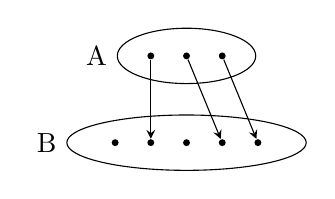
\begin{tikzpicture}
        [
            group/.style={ellipse, draw, minimum height=20pt,
                          minimum width=50pt, label=left:#1},
            dot/.style={circle, fill, minimum width=2.5pt, inner sep=0pt}
        ]
        \node (a) [dot] {};
        \node (b) [dot, right=10pt of a] {};
        \node (c) [dot, right=10pt of b] {};
        \node (q) [dot, below=of a] {};
        \node (r) [dot, below=of b] {};
        \node (s) [dot, below=of c] {};
        \node (p) [dot, left=10pt of q] {};
        \node (t) [dot, right=10pt of s] {};
        \foreach \i/\j in {a/q,b/s,c/t}
            \draw [->, >=stealth,scale=3] (\i) -- (\j);
        \node [fit=(a) (b) (c), group=A] {};
        \node [fit=(p) (q) (r) (s) (t), group=B] {};
    \end{tikzpicture}
    \end{center}
\end{minipage}%
\begin{minipage}[t]{0.50\textwidth}
    \begin{center}
    Surjection\\
    $\forall b \in B.\ \exists a \in A.\ f(a) = b$

    \vspace{15pt}
    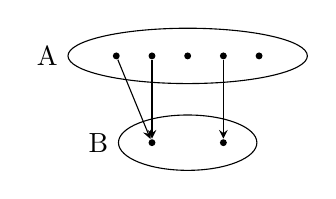
\begin{tikzpicture}
        [
            group/.style={ellipse, draw, minimum height=20pt,
                          minimum width=50pt, label=left:#1},
            dot/.style={circle, fill, minimum width=2.5pt, inner sep=0pt}
        ]
        \node (a) [dot] {};
        \node (b) [dot, right=10pt of a] {};
        \node (c) [dot, right=10pt of b] {};
        \node (d) [dot, right=10pt of c] {};
        \node (e) [dot, right=10pt of d] {};
        \node (p) [dot, below=of b] {};
        \node (q) [dot, below=of d] {};
        \foreach \i/\j in {a/p,b/p,d/q}
            \draw [->, >=stealth,scale=3] (\i) -- (\j);
        \node [fit=(a) (b) (c) (d) (e), group=A] {};
        \node [fit=(p) (q), group=B] {};
    \end{tikzpicture}
    \end{center}
\end{minipage}%
\end{example}


\begin{remark}
    Recall the universal problem of generating a monoid
    $(S^\ast, \epsilon, \cdot)$ from a set $S$ with a function
    $\sigma: S\to S^\ast$. Compare the definition of a universal solution to
    this problem: for all monoids $(M, \shortmid, \star)$,
    \begin{alignat*}{3}
        & \forall\, \text{functions } f:S\to M.\ &&
        \exists!\ \text{homomorphism }
        f^\#: (S^\ast, \epsilon, \cdot)
        \to
        (M, \shortmid, \star)
        .\ &&
        \textcolor{blue}{(}f^\#\textcolor{blue}{) \comp \sigma} = f
        %\\
        %& \forall\, y \in Y.\ &&
        %\exists!\ x \in X.\ &&
        %g(x) = y
    \end{alignat*}
    with the definition of a bijection $g : X \rightarrow Y$:
    \begin{alignat*}{3}
        %& \forall\, \text{functions } f:S\to M.\ &&
        %\exists!\ \text{homomorphism } f^\#:S^* \to M.\ &&
        %f = f^\# \comp \sigma
        %\\
        &
        \forall\, y \in Y.\
        \hspace*{2.5cm}
        &&
        \exists!\ x \in X.\
        \hspace*{5cm}
        &&
        \textcolor{blue}{g(}x\textcolor{blue}{)} = y
    \end{alignat*}

    The similarity suggests that solving an initial universal problem amounts
    to establishing a bijection that \emph{naturally converts} potential
    solutions (in the above example functions between the sets $S$ and $M$) to
    morphisms from the initial universal solution \big(in the above example
    homomorphisms between the monoids $(S^\ast, \epsilon, \cdot)$ and
    $(M, \shortmid, \star)$\big).
    %
    To see this, consider the hom-set of the generated monoid and any other
    monoid $(M, \shortmid, \star)$
    \begin{equation*}
        H_{\catmon}
        = \catmon \big( (S^*, \epsilon, \cdot), (M, \shortmid, \star) \big)
    \end{equation*}
    and the hom-set of our generating set $S$ and the underlying set $M$ of
    the proposed monoid:
    \begin{equation*}
        H_{\catset} = \catset ( S, M )
    \end{equation*}

    The universality condition
    \begin{center}
    \begin{tikzcd}
          S \arrow[r, "\sigma"]  \arrow[rd, swap, "\forall\, f"]
        &
        S^\ast
        \arrow[d, "f^\#"]
        & (S^\ast, \epsilon, \cdot)
        \arrow[d, "\exists!\, f^\# \text{ homomorphism}"]
        \\
        {} & M & (M, \shortmid, \star)
    \end{tikzcd}
    \end{center}
    states that for each function $f \in H_{\catset}$
    we must have a unique $f^\# \in H_{\catmon}$ such that $f = f^\# \comp
    \sigma$.  That is, we must have that the \emph{natural} function
    between $H_{\catmon}$ and $H_{\catset}$ given by
    \begin{equation*}
      \textcolor{blue}{(}-\textcolor{blue}{)\comp\sigma}:
      \catmon \big( (S^*, \epsilon, \cdot), (M, \shortmid, \star) \big)
      %\stackrel\cong
      \longrightarrow
      \catset ( S, M )
    \end{equation*}
    is a bijection.
\end{remark}

\section{Sections and retractions}

\begin{definition}[Sections and retractions]
A \emph{section} $s : A \morpharrow B$ is an arrow for which there exists an
arrow $r : B \morpharrow A$ (a \emph{retraction}) such that
\[
    r \comp s = \id{A}
\]
In other words, a section is the right inverse of some morphism.
Dually, a retraction is the left inverse of some morphism.
\end{definition}

\begin{example}
Consider the category of sets, $\catset$.

\begin{center}
    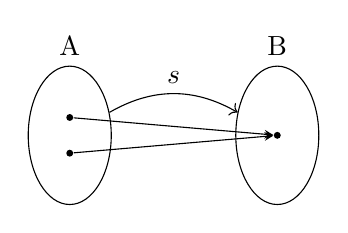
\begin{tikzpicture}
        [
            group/.style={ellipse, draw, minimum height=50pt,
                          minimum width=30pt, label=above:#1},
            dot/.style={circle, fill, minimum width=2.5pt, inner sep=0pt}
        ]
        \node (a) [dot] {};
        \node (b) [dot, below=10pt of a] {};
        \node (p) [dot, xshift=75pt] at ($(a)!1/2!(b)$) {};
        \foreach \i/\j in {a/p,b/p}
            \draw [->, >=stealth,scale=3] (\i) -- (\j);
        \node (A) [fit=(a) (b), group=A] {};
        \node (B) [fit=(p), group=B] {};
        \draw [->] (A) to [bend left] node[above] {$s$} (B);
    \end{tikzpicture}
\end{center}

The above map $s : A \morpharrow B$ can not be a section, as there is no way
to functionally ``go back to two points``.
Hence, a section in $\catset$ must at least be an injection.
However, note that if $A$ is the empty set, $s$ can not be a section.

In $\catset$, $s: A \to B$ is a section iff $s$ is injective and
($A = \emptyset \Rightarrow B = \emptyset$).

A map $r : B \rightarrow A$ is a retraction iff it has a section.
In $\catset$, retractions are the same as surjections (expressed
diagrammatically below).

\begin{center}
    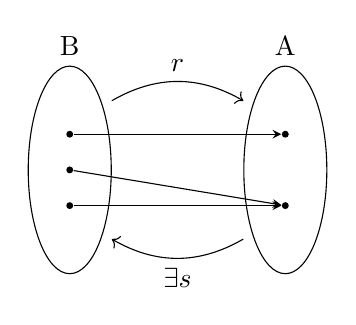
\begin{tikzpicture}
        [
            group/.style={ellipse, draw, minimum height=75pt,
                          minimum width=30pt, label=above:#1},
            dot/.style={circle, fill, minimum width=2.5pt, inner sep=0pt}
        ]
        \node (a) [dot] {};
        \node (b) [dot, below=10pt of a] {};
        \node (c) [dot, below=10pt of b] {};
        \node (p) [dot, right=75pt of a] {};
        \node (q) [dot, right=75pt of c] {};
        \foreach \i/\j in {a/p,b/q, c/q}
            \draw [->, >=stealth,scale=3] (\i) -- (\j);
        \node (B) [fit=(a) (b) (c), group=B] {};
        \node (A) [fit=(p) (q), group=A] {};
        \draw [->] ([yshift=25pt]B.east) to [bend left] node[above] {$r$}
                   ([yshift=25pt]A.west);
        \draw [->] ([yshift=-25pt]A.west) to [bend left] node[below]
                   {$\exists s$} ([yshift=-25pt]B.east);
    \end{tikzpicture}
\end{center}

\end{example}

\subsection{Axiom of choice}
\begin{center}
    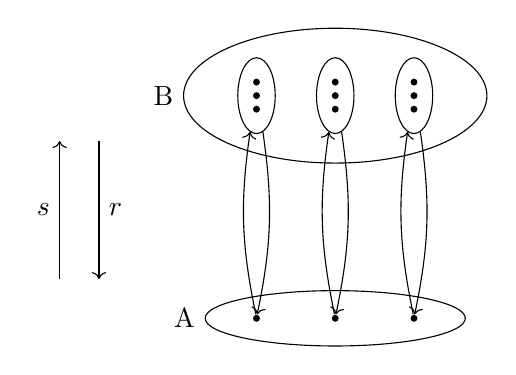
\begin{tikzpicture}
        [
            group/.style={ellipse, draw, minimum height=20pt,
                          minimum width=10pt, label=left:#1},
            dot/.style={circle, fill, minimum width=2.5pt, inner sep=0pt}
        ]
        \foreach \i [count = \xi] in {x,y,z}{
            \node (\i1) [dot] at (\xi, 0) {};
            \node (\i2) [dot,below=2pt of \i1] {};
            \node (\i3) [dot,below=2pt of \i2] {};
            \node (g-\i) [fit=(\i1) (\i2) (\i3), group] {};
            \node (a-\i) [dot] at (\xi, -3) {};
            \draw [->] (g-\i) to [bend left=10] (a-\i);
            \draw [->] (a-\i) to [bend left=10] (g-\i);
        }
        \node (A) [fit=(a-x) (a-y) (a-z), group=A] {};
        \node (B) [fit=(g-x) (g-y) (g-z), group=B] {};
        \draw [->] (-1.5,-2.5) to node[left] {$s$} (-1.5,-0.75);
        \draw [->] (-1.0,-0.75) to node[right] {$r$} (-1.0,-2.5);
    \end{tikzpicture}
\end{center}

The function $r$ has a section if, $\forall a \in A$, we can find a $b \in B$
such that $r(b) = a$.  In other words, $\forall a \in A$, a section $s$ is
defined by choosing $s(a) \in B$ such that $r\big(s(a)\big) = a$.  This may
require the \emph{axiom of choice}.

\begin{definition}
A category $\mathcal{C}$ \emph{satisfies the axiom of choice} whenever every
``surjection'' (technically, \emph{epimorphism}) in $\mathcal{C}$ has a
retraction.
\end{definition}

\section{Injections (technically, \emph{monomorphisms}) in categories}

A function $f : A \rightarrow B$ is \emph{injective} if every element in its
codomain is mapped to by at most one element in its domain:

\begin{equation*}
    \forall a, a' \in A.\ f(a) = f(a') \implies a = a'
\end{equation*}

How could we express this notion categorically? The set-theoretic definition
involves talking about function application and individual \emph{elements} of
sets, which do not in general exist in an arbitrary category. To avoid these
set-specific notions, we attempt to construct a definition which only mentions
morphisms and the operation of morphism composition.

\subsection{Proposed solution 1: morphisms from the terminal object
  (technically, \emph{global elements})}

In the category of sets, there is a bijection between the elements of a set
$S$ and the functions from a singleton set $\setof{*}$ to $S$: mapping $*$ to
an $s \in S$ amounts to selecting the specific element $s$ in $S$. This lets
us abstract over the notion of individual elements and is therefore a good
starting point for generalising the problem to categories. Before that, we
also need a category-theoretic counterpart to singleton sets:
\emph{terminal objects}.

\begin{definition}[Terminal objects]
A \emph{terminal object} in a category $\mathcal C$ is an object $\nelem{1}$
such that
\begin{equation*}
    \forall c \in \Ob(\mathcal C).\ \exists!\, u : c \rightarrow \nelem{1}
\end{equation*}
\end{definition}

A terminal object in $\catset$ is any singleton set, for instance $\{*\}$, as
for every other set $S$ we only have the constant function
$S \rightarrow \{*\}$ mapping $s \in S$ to $*$.
As with all universal constructions, all terminal objects in a category are
isomorphic to each other, so we can talk about \emph{the} terminal object.

Looking back at the definition of injections, we can use the terminal object
of a category to specify two ``elements'' of an object $A$ by as two morphisms
$a$ and $a'$ from $\nelem{1}$ to $A$.

\begin{center}
\begin{tikzcd}
    \nelem{1} \arrow[r, shift left=5pt, "a"]
               \arrow[r,shift right=5pt, swap, "a'"]
    & A \arrow[r, "f"]
    & B
\end{tikzcd}
\end{center}

The application of the function $f$ to the elements $a$ and $a'$ is translated
into composition of the morphisms $a$ and $a'$ with $f$.  We are thus lead to
the following:

\begin{equation*}
    \forall a, a' : \nelem{1} \rightarrow A.\ f \comp a = f \comp a'
    \implies a = a'
\end{equation*}

Unfortunately, this definition is too weak to capture the notion of
``injectivity'' for morphisms: the objects of a category may have internal
structures that cannot be ``selected'' by a morphism from the terminal
object.  Such a category is introduced in Exercise~\ref{lecture-5-exercise}.

\subsection{Proposed solution 2: morphisms from an arbitrary object
  (technically, \emph{generalized elements})}

To fix the issue in the previous definition, we consider mappings from any
object in the category, not just terminal objects.

\begin{definition}
A morphism $f: A\to B$ in a category $\mathcal C$ is said to be a
\emph{monomorphism} whenever
\begin{equation*}
    \forall X \in \Ob(\mathcal C).\
    \forall a, a' : X \rightarrow A \text{ in }\mathcal C.\
      f \comp a = f \comp a' \implies a = a'
    \enspace.
\end{equation*}
\end{definition}

Note how this definition of ``injectivity of morphisms'' (technically
monomorphisms) does not use any set-specific concepts such as elements and
function application: everything is expressed using composition of morphisms
which is available in any category.

\begin{exercise} \label{lecture-5-exercise}
Consider the category of \emph{directed graphs}, $\catdirgraph$:

\begin{itemize}
    \item Objects: tuples $(N, E, s, t)$ where $N$ is the set of nodes, $E$ is
      the set of edges and $s, t : E \rightarrow N$ are functions mapping an
      edge to its source and target nodes respectively.

    \item Morphisms from $G=(N,E,s,t)$ to $G'=(N',E',s',t')$: a pair of
      functions $(\eta, \varepsilon)$, where $\eta : N \rightarrow N'$ maps
      nodes to nodes and $\varepsilon : E \rightarrow E'$ maps edges to edges
      between two graphs such that connectivity is maintained:
      \begin{center}
      \begin{tikzcd}[row sep=0.8em]
      {}
      & E \arrow[ld, swap, "s"] \arrow[dd, "\varepsilon"] \arrow[rd, "t"]
      & {} \\
      N \arrow[dd, swap, "\eta"]
      & {}
      & N \arrow[dd, "\eta"] \\
      {}
      & E' \arrow[ld, "s'"] \arrow[rd, swap, "t'"]
      & {} \\
      N' & {} & N'
\end{tikzcd}
\end{center}
      That is, an
      edge $e$ between nodes $a$ and $b$ in the graph $G$ is mapped to an
      edge $\varepsilon(e)$ between the nodes $\eta(a)$ and $\eta(b)$ in the
      graph $G'$.
\begin{center}
\begin{tikzcd}[row sep=4em]
        a \arrow[r, swap, "e"{name=U}] \arrow[d, dashed, "\eta", mapsto]
      & b \arrow[d, dashed, "\eta", mapsto]
      & \text{in $G$}
      \\
        \eta(a) \arrow[r, "\varepsilon(e)"{name=D}]
      & \eta(b)
      \arrow[from=U, to=D, dashed, "\varepsilon", mapsto]
      & \text{in $G'$}
\end{tikzcd}
\end{center}
\end{itemize}

What is the terminal object of this category? It contains a single node (as the
singleton set is the terminal object of the set of nodes) and a single looping
edge:

\begin{center}
\begin{tikzcd}
    \bullet \arrow[out=150,in=210, loop, looseness=5]
\end{tikzcd}
\end{center}

In the category $\catdirgraph$, the notion of ``subgraph up to renaming'' is
captured by morphisms $(\eta,\varepsilon)$ such that both $\eta$ and
$\varepsilon$ are injections.
\begin{enumerate}
  \item
    Show that proposed solution 1 is insufficient to characterise the notion
    of subgraph up to renaming.  (Hint: Consider what structures can this
    single loop graph ``select'' from a graph.)
  \item
    Show that proposed solution 2 precisely characterises the notion of
    subgraph up to renaming.
\end{enumerate}
\end{exercise}


\chapter{Functors (definition)}
\lecturedetails{24 October 2017}{M Fiore, J Clarke, T Parks}

\section{Duality}
\begin{definition}[Duality]
Given a category $\mathcal{C}$, we define the \emph{opposite} or \emph{dual}
category, $\mathcal{C}^{\op}$, to be the category with:
    \begin{itemize}
        \item $\Ob(\mathcal{C}^{\op}) = \Ob(\mathcal{C})$
        \item $\mathcal{C}^{\op}(A, B) \eqdef \mathcal{C}(B, A)$
    \end{itemize}

\begin{minipage}[t]{0.49\textwidth}
    \begin{center}
        In $\mathcal{C}^{\op}$

        \vspace{15pt}

        \begin{tikzcd}
            A \arrow[d, swap, "f"] \\
            B
        \end{tikzcd}
    \end{center}
\end{minipage}%
\vline%
\begin{minipage}[t]{0.49\textwidth}
    \begin{center}
        In $\mathcal{C}$

        \vspace{15pt}

        \begin{tikzcd}
            A \\
            B \arrow[u, "f"]
        \end{tikzcd}
    \end{center}
\end{minipage}

Identities are the same as in $\mathcal{C}$, that is:

\begin{equation*}
    \id{A}^{\op} \eqdef \id{A}
\end{equation*}

For composition, we need:

\begin{equation*}
    \equalto{\mathcal{C}^{\op}(B, C)}{\mathcal{C}(C, B)} \times
    \equalto{\mathcal{C}^{\op}(A, B)}{\mathcal{C}(B, A)}
    \xrightarrow{\comp^{\op}_{A,B,C}}
    \equalto{\mathcal{C}^{\op}(A, C)}{\mathcal{C}(C, A)}
\end{equation*}

Therefore, we define:

\begin{equation*}
    g \comp^{\op}_{A,B,C} f = f \comp_{C,B,A} g
\end{equation*}
\end{definition}

\begin{definition}[Monomorphism]
A \emph{monomorphism} in a category $\mathcal{C}$ is a map $f : A \to B$ such
that for all $X \in \Ob(\mathcal{C})$ and for all $a, a' : X \to A$,
$f \comp a = f \comp a' \implies a = a'$.
\end{definition}

\begin{definition}[Epimorphism]
An \emph{epimorphism} in a category $\mathcal{C}$ is a monomorphism in
$\mathcal{C}^{\op}$, \ie~$f : A \to B$ is an epimorphism if:
\[
    \forall T \in \Ob(\mathcal{C}) . \forall t, t' : B \to T .
    t \comp f = t' \comp f \implies t = t'
\]
Here, $T$ can be thought of as an object of ``tests''.
\end{definition}

\begin{exercise}
Show that, in $\catset$, epimorphisms are the same as surjections.
\end{exercise}

\begin{exercise}
Show that each of isomorphisms, epimorphisms, monomorphisms, sections and
retractions are closed under composition; \ie~if $f : A \to B$ and
$g : B \to C$ are in one of these classes, then so is $g \comp f : A \to C$.
\end{exercise}

\begin{exercise}
Prove the labelled inclusions:

\begin{center}
    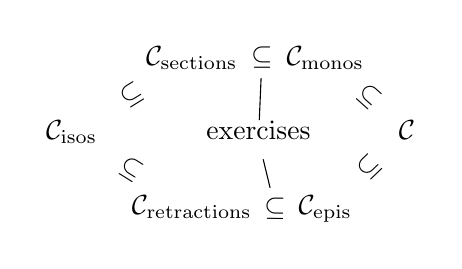
\begin{tikzpicture}
        \matrix[matrix of math nodes, name=m, column sep=0.6em, row sep=1.2em] {
            &
            |[alias=Sec]| \mathcal{C}_{\mathrm{sections}} &
            |[alias=Mono]| \mathcal{C}_{\mathrm{monos}} &
            \\
            |[alias=Cong]| \mathcal{C}_{\mathrm{isos}} &
            |[alias=Ex1]| &
            |[alias=Ex2]| &
            |[alias=C]| \mathcal{C}
            \\
            &
            |[alias=Ret]| \mathcal{C}_{\mathrm{retractions}} &
            |[alias=Epi]| \mathcal{C}_{\mathrm{epis}} &
            \\
        };

        \node (Ex) [fit=(Ex1)(Ex2)]{exercises};

        \path (Cong) edge[draw=none] node[sloped, allow upside down, auto=false] {$\subseteq$} (Sec)
              (Cong) edge[draw=none] node[sloped, allow upside down, auto=false] {$\subseteq$} (Ret)
              (Sec) edge[draw=none] node (SecMono) [sloped, allow upside down, auto=false] {$\subseteq$} (Mono)
              (Ret) edge[draw=none] node (RetEpi) [sloped, allow upside down, auto=false] {$\subseteq$} (Epi)
              (Mono) edge[draw=none] node[sloped, allow upside down, auto=false] {$\subseteq$} (C)
              (Epi) edge[draw=none] node[sloped, allow upside down, auto=false] {$\subseteq$} (C)
              (Ex) edge (SecMono)
              (Ex) edge (RetEpi);
    \end{tikzpicture}
\end{center}
\end{exercise}

Recall that the product of a family of objects $\setof{A_i \suchthat i \in I}$
is given by:

\begin{equation*}
    \left(\prod_{i\in I} A_i\right) \xrightarrow{\pi_k} A_k
    \qquad (k\in I)
\end{equation*}

such that it is a terminal universal solution.

\begin{definition}
\emph{Coproducts}, or \emph{sums}, in $\mathcal{C}$ are products in
$\mathcal{C}^{\op}$. The coproduct of a family
$\setof{A_i \suchthat i \in I}$ is given by

\begin{center}
    \begin{tikzcd}
        A_k \arrow[r, "\iota_k"] \arrow[dr, swap, "\forall f_k"] &
        \left(\coprod_{i \in I} A_i\right) \arrow[d, "\exists!f_k"]
        \\
        &
        X
    \end{tikzcd}
    \qquad$(k\in I)$
\end{center}
\end{definition}

In $\catset$, coproducts are disjoint unions:

\begin{equation*}
    \begin{aligned}
        \coprod_{i \in I} A_i \ = \ \bigcup_{i \in I}\, \setof{i} \times A_i &
        \overset{\iota_k}{\leftarrow} A_k
        \\
        (k, a) &
        \mapsfrom a
    \end{aligned}
\end{equation*}

\begin{exercise}
Calculate coproducts/sums in the categories introduced so far ($\catpfn$,
$\catrel$, $\catpred$, $\catpreo$, $\catmon$, \dots).
\end{exercise}

\begin{exercise}
Prove or disprove whether bijections ($\iffdef$ monomorphic and epimorphic) are
the same as isomorphisms.
\end{exercise}

\section{Functors}

Categories are mathematical structures with their own morphisms,
\emph{functors}:
\begin{center}
\begin{tikzcd}
    \mathcal{A} \arrow[r, "F"]  & \mathcal{B}
\end{tikzcd}
\end{center}
We will motivate their definition by considering two special kinds of
categories, monoids and preorders, together with their respective morphisms.

\subsection{Monoids can be regarded as categories}

A monoid $(M, \shortmid, \star)$ maybe seen as the category $\mathcal M$ with
a single object:
\begin{align*}
\Ob(\mathcal M) &\eqdef \setof{ \bullet }
\end{align*}
for which the hom-set consists of the elements of the monoid:
\begin{align*}
\mathcal{M}(\bullet, \bullet) &\eqdef M
\end{align*}
The identity is the neutral element of the monoid:
\begin{align*}
\id{\bullet} &\eqdef\ \shortmid
\end{align*}
and the composition of morphisms is the monoid multiplication:
\begin{align*}
f \comp g &\eqdef f \star g
\enspace.
\end{align*}

Conversely, every category $\mathcal C$ with a singleton set of objects, say
$\setof{\bullet}$, has an underlying monoid structure given by
\[
  \big(\, \mathcal{C}(\bullet,\bullet) \,,\, \id{\bullet} \,,\, \comp \,\big)
\]

The above two constructions are in bijective correspondence.

\subsection{Preorders can be regarded as categories}

For a preorder $(P, \leq)$, consider the category $\mathcal P$ with
$\Ob(\mathcal P) = P$ and hom-sets
\[
\mathcal{P}(p, q)
= \begin{cases}
    \bigsetof{\, (p,q) \,} & \text{if } p \leq q
    \\[1mm]
    \emptyset & \text{otherwise }
  \end{cases}
\qquad
(p,q \in P)
\]

As $p \leq p$, the identity is given by
\begin{align*}
\id{p} &\eqdef (p,p)
\end{align*}

We also need to consider the operation of composition:
\[
\mathcal{P}(q, r) \times \mathcal{P}(p, q) \to \mathcal{P}(p, r)
\]
We can determine it by cases:
\begin{itemize}
\item
If either $\mathcal{P}(q, r)$ or $\mathcal{P}(p, q)$ are empty, then so is
$\mathcal{P}(q, r) \times \mathcal{P}(p, q)$ and the composition map is
uniquely determined.

\item
Otherwise, both $\mathcal{P}(q, r)$ and $\mathcal{P}(p, q)$ are singleton
sets so that, by the transitivity property of preorders, so is
$\mathcal{P}(p, r)$; and the composition map is again uniquely determined.
\end{itemize}

Conversely, every category $\mathcal C$ with a set of objects and
subsingleton~(\viz,~a subset of a singleton) hom-sets has an underlying
preorder structure given by
\[
  \big(\, \Ob(\mathcal C) \,,\, \leq \,\big)
\]
where $X \leq Y \iffdef ( \mathcal{C}(X, Y) \iso \nelem 1 )$.

\paragraph{Locally small and small categories.}
%
The notion of category we have considered, with a class of objects and
hom-sets, is technically referred to as \emph{locally small}.  Categories with
a set of objects are referred to as \emph{small}.  The categories associated
to monoids and preorders are small.

\subsection{Morphisms of monoids, preorders, and categories}

We recall the notions of morphism between monoids and preorders, and
generalize them to categories.

\begin{center}\begin{tabular}{ccc}
Monoids and homomorphisms & \qquad\qquad\qquad & Preorders and monotone
functions
\\[3mm]
$(M_1, \shortmid_1, \star_1)
 \stackrel{h}{\longrightarrow}
 (M_2, \shortmid_2, \star_2)$
&&
$(P_1, \leq_1) \stackrel{f}{\longrightarrow} (P_2, \leq_2)$
\\[3mm]
\begin{tabular}{l}
$h: M_1 \to M_2$
\\[1mm]
s.t.~$h(\shortmid_1) =\ \shortmid_2$
\\[1mm]
\phantom{s.t.~}$h(x \star_1 y) = h(x) \star_2 h(y)$
\end{tabular}
&&
\begin{tabular}{l}
$f: P_1 \to P_2$
\\[1mm]
s.t.~$p \leq_1 q \implies f(p) \leq_2 f(q)$
\end{tabular}
\end{tabular}
\end{center}

\begin{center}\begin{tabular}{c}
Categories and functors
\\[3mm]
$\mathcal{C}_1 \stackrel{F}{\longrightarrow} \mathcal{C}_2$
\\[4mm]
$\left\{
\begin{array}{l}
F_{\textrm{obj}} : \Ob(\mathcal{C}_1) \to \Ob(\mathcal{C}_2)
\\[3mm]
F_{\textrm{arr}} : \Arr(\mathcal{C}_1) \longrightarrow \Arr(\mathcal{C}_2)
\end{array}
\right.$
\\[8mm]
\begin{tabular}[t]{lc}
s.t. &
\\
&
% the yshift is needed to make the F_arrow level.
\begin{tikzcd}
P
\arrow[dd, "f"{name=L, right}] & & F_{obj}(P)
\arrow[dd, "F_{\text{arr}}(f)"{name=R, left}]
\\
\arrow[rr, "F_{arr}", from=L, to=R, start anchor={[yshift=-0.2ex]}, mapsto]
&  &
\\
Q &  & F_{obj}(Q)
\end{tikzcd}
\\[20mm]
&
$F_{\textrm{arr}}( \id{X} ) \,=\, \id{ F_{\textrm{obj}}(X) }$
\\[6mm]
&
\begin{tikzcd}
A \arrow[d, "f"] \arrow[dd, "g \comp f"', bend right=50]
&
F_\text{obj}(A)
\arrow[d, "F_\text{arr}(f)"{left}]
\arrow[dd, "F_\text{arr}(g \comp f)", bend left=55]
\\
B \arrow[d, "g"] & F_\text{obj}(B) \arrow[d, "F_\text{arr}(g)"{left}]
\\
C & F_\text{obj}(C)
\end{tikzcd}
\end{tabular}
\end{tabular}\end{center}


\chapter{Functors (examples)}
\lecturedetails{26 October 2017}{M Fiore, N Alcock, Z Yuan}

\section{Functors (enriched viewpoint)}

\begin{definition}
A functor \(F: \mathcal{A} \rightarrow \mathcal{B}\) is given by a mapping
\(F: \Ob(\mathcal{A}) \rightarrow \Ob(\mathcal{B})\) together with a family of
functions \(F_{X,Y}: \mathcal{A}(X, Y) \rightarrow \mathcal{B}(FX, FY)\) for
all \(X, Y \in \Ob(\mathcal{A})\), so that

\begin{center}
\begin{tabular}[t]{lc}
\\
&
% the yshift is needed to make the F_arrow level.
\begin{tikzcd}
X
\arrow[dd, "\mathcal{A}\ni f"{name=L, right}]
& \qquad & FX
\arrow[dd, "F_{X,Y}(f)\in\mathcal{B}"{name=R, left}]
\\
&
\arrow[rr, "F_{X,Y}", from=L, to=R, %start anchor={[yshift=-0.2ex]},
mapsto]
& &
\\
Y &  & FY
\end{tikzcd}
\\[20mm]
\end{tabular}
\end{center}

such that the following two diagrams commute:

\begin{center}
    \begin{tikzcd}
        \nelem{1} \arrow[r, "id^{(\mathcal{A})}_A"]
        \arrow[dr, swap, "id^{(\mathcal{B})}_{FA}"] &
        \mathcal{A}\left(A,A\right) \arrow[d, "F_{A,A}"]
        \\
        &
         \mathcal{B}\left(FA,FA\right)
    \end{tikzcd}
\end{center}

\begin{center}
    \begin{tikzcd}[ampersand replacement=\&]
        \mathcal{A}(Y,Z) \times  \mathcal{A}(X,Y)
        \arrow[r, "\circ_{X,Y,Z}^{(\mathcal{A})}"]
        \arrow [d, "F_{Y,Z} \times F_{X,Y}"{left}] \&
        \mathcal{A}(X,Z)
        \arrow[d, "F_{X,Z}"] \&
        \\
        \mathcal{B}(FY,FZ) \times  \mathcal{B}(FX,FY)
        \arrow[r, "\circ_{FX,FY,FZ}^{(\mathcal{B})}"] \&
        \mathcal{B}(FX,FZ) \&
    \end{tikzcd} \\[3mm]
\end{center}
\end{definition}

\begin{remark}
Compare the above with the notion of monoid homomorphism:
\begin{center}
    \begin{tikzcd}
        \nelem{1} \arrow[r, "\shortmid_1"] \arrow[dr, swap, "\shortmid_2"] &
       M_1 \arrow[d, "h"]
        \\
        &
         M_2
    \end{tikzcd}
\end{center}

\begin{center}
    \begin{tikzcd}[ampersand replacement=\&]
        M_1 \times M_1 \arrow[r, "\star_1"] \arrow [d, "h \times h"{left}] \&
        M_1 \arrow[d, "h"] \&
        \\
        M_2 \times M_2 \arrow[r, "\star_2"] \&
        M_2 \&
    \end{tikzcd} \\[3mm]
\end{center}
\end{remark}

\section{Examples}

\subsection{Identity functor}

For any category $\lscat{C}$, $\fncid{\lscat{C}}: \lscat{C} \to \lscat{C}$ is
the functor that maps both objects and morphisms to themselves.

\begin{center}
\begin{tikzcd}
A \arrow[dd, "f" swap] & A \arrow[dd, "f"] \\
{} \arrow[r, mapsto, "\fncid{}"] & {}\\
B & B
\end{tikzcd}
\end{center}

\subsection{List functor}

Recall the universal property of the free monoid on a set
\begin{center}
\begin{tikzcd}
  S \arrow[r, "\eta_S"]  \arrow[rd, swap, "\forall\, f"]
  &
  \fnclist(S)
  \arrow[d, "f^\#"]
  & (\fnclist(S), nil, @)
  \arrow[d, "\exists!\, f^\# \text{ homomorphism}"]
  \\
  {} & M & \forall (M, \shortmid, \star) \text{ monoid}
\end{tikzcd}
\end{center}
giving rise to the list construction.

We have a \emph{list functor} \(\fnclist: \catset \to \catset\) informally
given as follows:
\begin{center}
\begin{tabular}[t]{lc}
\\
&
% the yshift is needed to make the F_arrow level.
\begin{tikzcd}
A
\arrow[dd, "f"{name=L, right}] & & List(A)
\arrow[dd, "\fnclist(f)"{name=R, left}]
\\
\arrow[rr, "\fnclist{}", from=L, to=R, start anchor={[yshift=-0.2ex]}, mapsto]
&  &
\\
B &  & \fnclist(B)
\end{tikzcd}
where $\fnclist(f) \eqdef \map{f}$
\begin{tikzcd}
        \big[\, a_1, ... ,a_n \,\big]
        \arrow[d, "",mapsto]
        \\
        \big[\, f(a_1), ... , f(a_n) \,\big]
    \end{tikzcd}
\\[20mm]
\end{tabular}
\end{center}

Functoriality amounts to checking that
\[\map{\,\id{A}} = \id{\fnclist(A)}\]
and
\[\map{g} \comp \map{f} = \map{g \comp f}\enspace.\]\\
By definition of \(\map\), it is easy to show that
\(\map{\,\id{A}} = \id{\fnclist(A)}\), and we also have:
\begin{center}
    \begin{tikzcd}[ampersand replacement=\&]
        \big[\, a_1, ... ,a_n \,\big] \arrow [d, "map(f)" ,start anchor={[yshift=-0.2ex]}, mapsto]  \arrow[rd, "map(g \circ f)", mapsto]\&
           \\
        \big[\, f(a_1), ... , f(a_n) \,\big] \arrow[r, "map(g)", mapsto] \&
         \big[\, g(f(a_1)), ... , g(f(a_n)) \,\big] =  \big[\, (g\circ f)(a_1), ... , (g\circ f)(a_n) \,\big] \&
    \end{tikzcd} \\[3mm]
\end{center}

Let us show that $\fnclist$ is a functor solely from the universal property of
a free monoids.

Firstly, we define the action of the functor on morphisms as follows:
\begin{center}
    \begin{tikzcd}[ampersand replacement=\&]
        A \arrow[r, "{[\phold]_A}"] \arrow [d, "f"{left}] \&
        \fnclist(A)
        \arrow[d, "\fnclist(f)\eqdef {\big([\phold]_B\circ f\big){^\#}}"]
        \& \qquad \&
        (\fnclist(A), nil, @)
        \arrow[d, "\exists!\ {\big([\phold]_B\circ f\big)^{\#}}
          \text{ homomorphism}" ]
           \\
        B \arrow[r, "{[\phold]_B}"] \&
        \fnclist(B) \& \& (\fnclist(B), nil, @)
    \end{tikzcd} \\[3mm]
\end{center}

We now check functoriality.
\begin{itemize}
\item Preservation of identities:
\begin{center}
    \begin{tikzcd}[ampersand replacement=\&]
        A \arrow[r, "{[\phold]_A}"]
        \arrow [d, "\id{A}"{left}]
        \&
        \fnclist(A)
        \arrow[d, "{\fnclist(\id{A}) \eqdef \big([\phold]_A\big)^\#}"]
        \& \&
        (\fnclist(A), nil, @)
        \arrow[d,
          "{\exists! \text{ homomorphism }
              \big([\phold]_A\big)^\# \,= \ \id{\fnclist(A)}}"]
        \\
        A \arrow[r, "{[\phold]_A}"] \&
        \fnclist(A) \& \& (List(A), nil, @)
    \end{tikzcd} \\[3mm]
\end{center}

\item Preservation of composition:
\begin{center}
\begin{tikzcd}
    A
    \arrow[d, "f"]
    \arrow[dd, bend right=40, "g \comp f" swap]
    \arrow[r, "{[\phold]_A}"]
    &
    \fnclist(A)
    \arrow[d, dotted, "\fnclist(f)"]
    \arrow[dd, bend left=80, dotted, "\fnclist(g) \comp \fnclist(f)"]
    \\
    B
    \arrow[d, "g"]
    \arrow[r, "{[\phold]_B}"]
    &
    \fnclist(B)
    \arrow[d, dotted, "\fnclist(g)"]
    \\
    C \arrow[r, "{[\phold]_C}"]
    &
    \fnclist(C)
\end{tikzcd}
\end{center}

Note that $\fnclist(g) \comp \fnclist(f)$ is an homomorphism \big(because so
are $\fnclist(g)$ and $\fnclist(f)$\big) such that
$\big(\fnclist(g) \comp \fnclist(f) \big)\comp {[\phold]_A}
 = {[\phold]_C} \comp (g \comp f)$.  Therefore,
\[
 \fnclist(g) \comp \fnclist(f)
 \ = \  \big( {[\phold]_C} \comp (g \comp f) \big)^\#
 \ \eqdef \ \fnclist(g\comp f)
  \enspace.
\]
\end{itemize}

\begin{exercise}\label{ex:fcmonoidfunctor}
Show that the free commutative monoid (\ie~finite multiset) construction
\begin{center}
    \begin{tikzcd}
          S \arrow[r, "\setof{\phold}_S"]  \arrow[rd, swap, "\forall\, f"]
        &
        \mathcal M_f(S)
        \arrow[d, "f^\#"]
        & (\mathcal M_f(S),\emptyset,\oplus)
        \arrow[d, "\exists!\text{ homomorphism } f^\#"]
        \\
        {} & C & (C,\shortmid,\star) & \forall\ \text{commutative monoid}
    \end{tikzcd}
    \end{center}
yields a functor.
\end{exercise}

\begin{exercise}\label{ex:fsemilatticefunctor}
Show that the free semilattice [equivalently, free commutative and idempotent
monoid] (\ie~finite powerset) construction yields a functor.
\end{exercise}

\section{Products and coproducts}

\subsection{$\catcat$}

\begin{definition}
The (locally small) category \(\catcat\) has as objects small categories and
as morphisms functors.  Identities are given by the identity functors
\(\Id{\mathbb{C}}\) and the composition of
\(\mathbb{A} \morpharr{F} \mathbb{B} \morpharr{G} \mathbb{C}\) is the functor
$G\comp F:\mathbb A\to \mathbb C$ defined by setting
\((G \comp F)(-) \eqdef G(F(-))\) both on objects and morphisms.
\end{definition}

The terminal object in \(\catcat\) is the one-object one-arrow category:
\begin{center}
\begin{tikzcd}
    \star \arrow["\id{\Large\star}", out=150,in=210, swap, looseness=5]
\end{tikzcd}
\end{center}

\begin{definition}[Product category]
The product of two categories $\lscat{A}$ and $\lscat{B}$, denoted
$\lscat{A}\times\lscat{B}$, is the category whose objects are pairs $(A, B)$
with $A \in \Ob(\lscat{A})$ and $B \in \Ob(\lscat{B})$, and whose morphisms
$(A', B') \to (A', B')$ are pairs $(f,g)$ of arrows with $f:A\to A'$ in
$\lscat A$ and $g:B\to B'$ in $\lscat B$.  Identities and composition are
given pointwise: $\id{(A, B)} = (\id{A}, \id{B})$ and
$(f, g) \comp (f', g') = (f \comp f', g \comp g')$.
\end{definition}

\begin{center}
\begin{tikzcd}
  (A_1,B_1)
  \arrow[r, "{(f,g)}"]
  \arrow[rr, swap, bend right=30,
    "{(f',g')\circ(f,g) \ \eqdef \ (f'\circ f, g'\circ g)}"]
  &
  (A_2,B_2)
  \arrow[r, "{(f',g')}"]
  &
  (A_3,B_3)
\end{tikzcd}
\end{center}

Recall the definition of binary products in a category:
\begin{equation}\label{UniversalPairingMap}
\begin{tikzcd}
    {} & P \arrow[ld, swap, "\pi_1"] \arrow[rd, "\pi_2"] & {} \\
    A
    & {}
    &
    B
    \\
    {} &
    \stackrel{\mbox{$C$}}{\forall}
    \arrow[uu, dashed, "\exists!", "{\univpair{f,g}}" swap]
    \arrow[lu, "\forall\, f"] \arrow[ru, swap, "\forall\, g"] & {}
\end{tikzcd}
\end{equation}

\begin{exercise}\label{ex:produnivconstr}
Show that the product of categories $\lscat A\times\lscat B$ equipped with the
projection functors
\begin{center}
\begin{tikzcd}
    {} & {\lscat{A}\times\lscat{B}}
    \arrow[ld, swap, "\pi_1"] \arrow[rd, "\pi_2"] & {}
    \\
    \lscat{A} & {} & \lscat{B}
\end{tikzcd}
\end{center}
given by
\begin{center}
\begin{tikzcd}
  &
  {(A, B)}
  \arrow[dd, "{(f, g)}"]
  \arrow[rd, "\pi_2", mapsto ,
    start anchor={[yshift=-6.5ex]},
    end anchor={[yshift=-6.5ex]}
    ]
  &
  \\
  A \arrow[dd, "f"{name=L}]
  &
    \arrow[l, "\pi_1"{left}, mapsto, to=L]
  &
  B \arrow[dd, "g"{left, name=R}]
  \\
  & {(A', B')} &
  \\
  A' & & B'
\end{tikzcd}
\end{center}
is universal.
\end{exercise}

\subsection{Product and coproduct functors}

\begin{remark}
The product and coproduct constructions are functors.
\end{remark}

Let \(\lscat{C}\) be a category with binary products for all pairs of objects,
and write
\begin{center}\begin{tikzcd}
    &
    \mathrm{Prod}(A, B)
    \arrow[ld, swap, "\pi^{A,B}_1"]
    \arrow[rd, "\pi^{A,B}_2"]
    &
    \\
    A & & B
\end{tikzcd}\end{center}
for a specified product of $A, B \in \Ob(\lscat{C})$.\

\begin{exercise}\label{ex:prodfunc}
For $f: A\to A'$ and $g:B\to B'$ in $\lscat C$, define
$\textrm{Prod(f,g)}:\textrm{Prod}(A,B)\to\textrm{Prod}(A',B')$ in $\lscat C$
to be the unique morphism (guaranteed to exist by the universal property of
products) as follows:
\begin{center}
\begin{tikzcd}
    {}
    & \mathrm{Prod}(A, B)
    \arrow[ld, swap, "\pi^{A,B}_1"]
    \arrow[rd, "\pi^{A,B}_2"]
    \arrow[ddd, dashed, "\exists!" swap, "{\textrm{Prod}(f, g)}"]
    & {}
    \\
    A \arrow[d, swap, "f"]
    & {} &
    B  \arrow[d, "g"]
    \\
    A' & {} & B'
    \\
    {} &
    \mathrm{Prod}(A', B') \arrow[lu, "\pi^{A',B'}_1"]
    \arrow[ru, swap, "\pi^{A',B'}_2"]
    & {}
\end{tikzcd}
\end{center}
that is, using the notation of~(\ref{UniversalPairingMap}),
\[
  \textrm{Prod}(f,g)
  \ \eqdef \
  \bigunivpair{\, f\comp\pi^{A,B}_1 \, , \, g\comp\pi^{A,B}_2 \,}
  \enspace.
\]
Show that the above definition yields a functor
$\textrm{Prod}:\lscat C\times\lscat C\to \lscat C$; \ie~show that
$\mathrm{Prod}(\id{A}, \id{B}) = \id{\mathrm{Prod}(A,B)}$ and that
$\mathrm{Prod}(f, g) \comp \mathrm{Prod}(f', g')
 = \mathrm{Prod}(f \comp f', g \comp g')$.
\end{exercise}

\subsection{Hom functor}

For a locally small category $\lscat C$, we define the \emph{hom functor}
$\lscat C(-, =): \lscat C^{op} \times \lscat C \to \catset$ mapping objects
from $\lscat C^{op} \times \lscat C$ to the set of morphisms between them:
$$
  A, B \mapsto \lscat C(A, B)
$$
and given on morphisms as follows
\begin{center}
  \begin{tikzcd}
    A 
    &
    B \ar["g"]{d}
    &
    &
    (A, B) \ar["{(f, g)}"{name=L}]{d}
    &
    \lscat C (A, B) 
    \ar["{\lscat C(f, g) \eqdef \lambda h. g \circ h \circ f}"{name=R}]{d}
    &
    &
    &
    A \overset h \longrightarrow B
    \\
    A' \ar["f"]{u}
    &
    B'
    &
    &
    (A', B')
    &
    \lscat C (A', B')
    &
    &
    &
    A' \overset  {g \circ h \circ f} \longrightarrow B'
    \ar[from=L, to=R, mapsto, shorten <= 2pt, shorten >= 2pt]
    \ar[from=1-8, to=2-8, mapsto, shorten <= 2pt, shorten >= 2pt]
  \end{tikzcd}
\end{center}


\chapter{Natural transformations}
\lecturedetails{31 October 2017}{M Fiore, V Chakraborty, N Licker}

Natural transformations are morphisms between functors with the same domain
and codomain.  

\section{Motivation}

In the category $\catpreo$, morphisms are monotone functions between
preorders.  These morphisms can in turn be pre-ordered:
\[
  f \le g : (P, \le_P) \to (Q, \le_Q)
  \iffdef \forall p \in P. f(p) \le g(p) \enspace.
\]

For categories, with morphisms between them given by functors, we have natural
transformations 
\[
  \varphi: F \Rightarrow G: \lscat A\to \lscat B
\]
that relate them.

\begin{center}
    \begin{tikzcd}[sep=6em]
      \lscat A
        \ar[bend left=40, "F"{name=T, above}]{r}
        \ar[bend right=40, "G"{name=B, below}]{r}
      &
      \lscat B
      \\
      \ar[Rightarrow, from=T, to=B, "{\varphi}", shorten <= 2pt, shorten >= 2pt]
    \end{tikzcd}\\[3mm]
\end{center}

\section{Definition}

\begin{definition}[Natural Transformations]

A natural transformation $\varphi: F \Rightarrow G : \lscat A \to \lscat B$ is
a family:
\[
  \varphi = \Big \{ \varphi_A : F A \to G A \Big \}_{A \in \Ob(\lscat A)}
\]
such that the following \emph{naturality} condition holds:
\begin{center}
    for all
    \enspace
    \begin{tikzcd}
        A \arrow [d, "f"] \\ A' 
    \end{tikzcd} 
    in $\lscat A$,
    the square 
    \enspace
      \begin{tikzcd}
        F A \arrow[r, "\varphi_A"] \arrow [d, "F f",swap] &
        G A \arrow[d, "G f"]
        \\
        F A' \arrow[r, "\varphi_{A'}",swap] &
        G A'
    \end{tikzcd}
    commutes in $\lscat B$
    \enspace.
\end{center}

\end{definition}

\section{Examples}

\subsection{For the $\fnclist$ functor}

Recall that the list functor \(\fnclist: \catset \to \catset\) is defined by:

\begin{center}
\begin{tikzcd}
A
\arrow[dd, "f"{name=L, right}] & & List(A)
\arrow[dd, "\fnclist(f)"{name=R, left}]
\\
\arrow[rr, "\fnclist{}", from=L, to=R, start anchor={[yshift=-0.2ex]}, mapsto]
&  &
\\
B &  & \fnclist(B)
\end{tikzcd}
\end{center}

where $\fnclist(f)$ is the unique homomorphism
$$
(List(A), nil, @) \to (List(B), nil, @)
$$
such that the following square commutes:
\begin{center}
\begin{tikzcd}
A
\arrow[d, "f",swap]
\arrow[r, "{[\phold]_A}"]
&
List(A)
\arrow[d, "List(f)"]
\\
B
\arrow[r, "{[\phold]_B}", swap]
&
List(B)
\end{tikzcd}
\end{center}

\begin{example}[List-singletons]
The family of list-singleton functions
$$
{[\phold]} 
= 
\bigsetof{\, {[\phold]}_A : A \to List(A) \,}_{A\in\catset}
$$

is a natural transformation from $\fncid{\catset}$ to $\fnclist$:

\begin{center}
    \begin{tikzcd}[sep=6em]
      \catset
        \ar[bend left=40, "\fncid{\catset}"{name=T, above}]{r}
        \ar[bend right=40, "\fnclist"{name=B, below}]{r}
      &
      \catset
      \\
      \ar[Rightarrow, from=T, to=B, "{[\phold]}", shorten <= 2pt, shorten >= 2pt]
    \end{tikzcd}\\[3mm]
\end{center}
\end{example}


\begin{example}[List flattening]
Let $\text{flat}_A : \fnclist\big(\fnclist(A)\big) \to \fnclist(A)$ be the
function that flattens lists.

The family of functions
\[
  \text{flat} 
  = \bigsetof{\, 
      \text{flat}_A: \fnclist\big(\fnclist(A)\big) \to \fnclist(A) 
    \,}_{A \in \catset}
\]
is a natural transformation:
\begin{center}
    \begin{tikzcd}[sep=6em]
      \catset
        \ar[bend left=40, "List \circ List"{name=T, above}]{r}
        \ar[bend right=40, "\fnclist"{name=B, below}]{r}
      &
      \catset
      \\
      \ar[Rightarrow, from=T, to=B, "{[\phold]}", shorten <= 2pt, shorten >= 2pt]
    \end{tikzcd}\\[3mm]
\end{center}
\end{example}

\begin{exercise}
Show that $\text{flat}$ is a natural transformation using its universal
definition as follows:
\begin{center}
    \begin{tikzcd}[sep=6em]
      \fnclist(A)
        \ar["{[\phold]}_{\fnclist(A)}"]{r}
        \ar["id_{\fnclist(A)}"below]{rd}
      &
      \fnclist\big(\fnclist(A)\big)
        \ar[" (id_{\fnclist(A)})^\# \ \eqdef \ \text{flat}_A"]{d}
      \\
      &
      List(A)
    \end{tikzcd}\\[3mm]
\end{center}
\end{exercise}

\subsection{Coproducts}

Let $\lscat C$ be a category with binary coproducts (or sums); that is, we
have 
\begin{center}
    \begin{tikzcd}%[sep=6em]
      &
      A + B
        \ar[dotted, "{\exists![f,g]}"]{dd}
      &
      \\
      A
        \ar["f",swap]{dr}
        \ar["\iota_1^{A,B}"above]{ru}
      &
      &
      B
        \ar["g"]{ld}
        \ar["\iota_2^{A,B}"above]{lu}
      \\
      & \overset{\mbox{$C$}}{\forall} & 
    \end{tikzcd}\\[3mm]
\end{center}
for every pair of objects $A,B$ in $\lscat C$.

We have a \emph{coproduct functor} $\lscat C \times \lscat C \to \lscat C$
mapping as follows 
\begin{center}
  \begin{tikzcd}
    (A,B) \ar["{(f,g)}"{right},name=L]{d} 
    & 
    A+B \ar["f+g"{left},name=R]{d} 
    \ar[mapsto,from=L,to=R,shorten >= 0pt,shorten <=30pt]
    \\
    (A',B') & 
    A'+B'
  \end{tikzcd}
\end{center}
and defined by:
\begin{center}
    \begin{tikzcd}[sep=3em]
      &
      A + B
        \ar[dotted, "{\exists!(f+g)}"]{ddd}
      &
      \\
      A
        \ar["f"]{d}
        \ar["\iota_1^{A,B}"above]{ru}
      &
      &
      B
        \ar["g"]{d}
        \ar["\iota_2^{A,B}"above]{lu}
      \\
      A'
        \ar["\iota_1^{A',B'}"below]{rd}
      &
      &
      B'
        \ar["\iota_2^{A',B'}"below]{ld}
      \\
      &
      A' + B'
      &
    \end{tikzcd}\\[3mm]
\end{center}

\begin{exercise}
Show that the families 
\[
\iota_i
=
\bigsetof{\,
  \iota_i^{A_1,A_2}: A_i \to A_1 + A_2 
  \,}_{(A_1,A_2) \in \lscat C \times \lscat C}
\qquad(i=1,2)
\]
are natural transformations:
\begin{center}
    \begin{tikzcd}[sep=4em]
      \lscat C \times \lscat C
        \ar[bend left=40, "\pi_i"{name=T, above}]{r}
        \ar[bend right=40, "+"{name=B, below}]{r}
      &
      \lscat C
      \\
      \ar[Rightarrow, from=T, to=B, "{\iota_i}", shorten <= 2pt, shorten >= 2pt]
    \end{tikzcd}
\end{center}
\end{exercise}


\begin{definition}[Codiagonal]
For $A \in \Ob(\lscat C)$, we define the \emph{codiagonal} 
$\nabla_A:A + A\to A$ as the unique map such that
\begin{center}
    \begin{tikzcd}
      &
      A + A
        \ar[dotted, "{\exists!\nabla_A}"]{dd}
      &
      \\
      A
        \ar["id"below]{rd}
        \ar["\iota_1^{A,A}"above]{ru}
      &
      &
      A
        \ar["id"]{ld}
        \ar["\iota_2^{A,A}"above]{lu}
      \\
      &
      A
      &
    \end{tikzcd}\\[3mm]
\end{center}
\end{definition}

\begin{exercise}
Show that 
$\nabla = \Big\{ \nabla_A:A + A \to A \Big\}_{A \in \lscat C}$ is a natural
transformation:  
\begin{center}
    \begin{tikzcd}
      &
      \lscat C \times \lscat C
        \ar["+"above]{rd}
      &
      \\
      \lscat C
        \ar[bend right=30, "\Id{\lscat C}"{name=B, below}]{rr}
        \ar["\Delta"above]{ru}
      &
      &
      \lscat C
      \arrow[Rightarrow, from=1-2,to=B,"\nabla", shorten <= 2pt, shorten >= 2pt]
    \end{tikzcd}\\[3mm]
\end{center}
where $\Delta:\lscat C\to\lscat C\times\lscat C$ is the 
\emph{diagonal functor} given by $\Delta(-)\eqdef(-,-)$.
\end{exercise}

\section{Functor Categories}

\begin{definition}[Functor Category]
Given categories $\lscat X$ and $\lscat A$, the \emph{functor category} 
$\lscat A^\lscat X$ \big(or $[\lscat X, \lscat A]$\big) is the category whose
objects are functors from $\lscat X$ to $\lscat A$ and whose morphisms in
$\lscat A^\lscat X(F, G)$ are natural transformations from $F$ to $G$.  The
identity morphism $id_F : F \Rightarrow F : \lscat X \to \lscat A$ is
$id_F = \lbrace id_{FX}: FX \to FX \rbrace_{X \in \Ob(\lscat X)}$.
Composition is defined as follows: in the situation
\[
    \begin{tikzcd}[sep=5em]
      \lscat X
        \ar[bend left=60, "F"{name=F, above}]{r}
        \ar["G"name=G]{r}
        \ar[bend right=60, "H"{name=H, below}]{r}
      &
      \lscat A \\
      \ar[Rightarrow, from=F, to=G, "\varphi", shorten <= 2pt, shorten >= -1pt]
      \ar[Rightarrow, from=G, to=H, "\gamma", shorten <= 2pt, shorten >= 2pt]
    \end{tikzcd}\\[-12mm]
\]
we let $\gamma \circ \varphi:F\Rightarrow H$ be given by
\[
\gamma \circ \varphi 
\eqdef
\bigsetof{\, 
  \gamma_X \circ \varphi_X 
  : F X \to H X 
  \,}_{X \in \Ob(\lscat X)}
\]
that is,\\[-8mm]
\begin{center}
    \begin{tikzcd}
      F X
        \ar["(\gamma \circ \varphi)_X \,\eqdef\, \gamma_X \circ \varphi_X"]{rr}
        \ar["\varphi_X",swap]{rd}
      &
      &
      H X
      \\
      &
      G X
        \ar["\gamma_X",swap]{ru}
      &
    \end{tikzcd}
\end{center}
\end{definition}

\begin{exercise}
Check that if $\varphi$ and $\gamma$ as above are natural transformations then
so is $\gamma \circ \varphi$ as defined.
\end{exercise}

\begin{example}
Consider the terminal category $\nelem 1$ and an arbitrary locally small
category $\lscat C$. The functor category $\lscat C^{\nelem1}$ has:
\begin{itemize}
  \item 
    Functors 
    \[
      \framebox{\begin{tikzcd}
          * \arrow[out=150,in=210, loop, looseness=5, "id_*"left]
      \end{tikzcd}}
      \longrightarrow 
      \lscat C
    \]
    from $\nelem 1$ to $\lscat C$ as objects; so that 
    \[
      \Ob(\lscat C^{\nelem1})\iso\Ob(\lscat C)
      \enspace.
    \]

  \item 
    Natural transformations 
    \[
      \varphi: F \Rightarrow G: \nelem 1 \to \lscat C
    \]
    between functors as morphisms; so that
    \[
      \varphi = \bigsetof{\, \varphi_* : F * \to G * \text{ in } \lscat C \,}
      \enspace.
    \]
\end{itemize}
\end{example}

\begin{exercise}
Prove that $\lscat C^{\nelem1} \iso \lscat C$.
\end{exercise}

\begin{example}
Let $\cat D$ be the category with two objects and a parallel pair of arrows:
\[
  \begin{array}{|c|}\hline 
  \begin{tikzcd}
    E
      %\arrow[out=150,in=210, loop, looseness=5, "id_*"left]
      \arrow[shift left=+2, "s"above]{r}
      \arrow[shift left=-2, "t"below]{r}
    &
    N %\arrow[out=30,in=-30, loop, looseness=5, "id_\bullet"right]
  \end{tikzcd}
  \\ \hline \end{array}
\]
where, as it is customary, identities have been omitted from the picture.

In the functor category $\catset^{\cat D}$, 
\begin{itemize}
\item
the objects are functors
\[
  \begin{array}{|c|}\hline 
  \begin{tikzcd}
  E \arrow[shift left=+2, "s"above]{r} \arrow[shift left=-2, "t"below]{r} 
  & N
  \end{tikzcd}
  \\ \hline \end{array}
  \overset G\longrightarrow 
  \catset 
\]
and therefore essentially given by sets and functions between them as follows:
\[
  \begin{tikzcd}[sep=4em]
  G(E) \arrow[shift left=+2, "G(s)"above]{r} 
  \arrow[shift left=-2, "G(t)"below]{r} & G(N)
  \end{tikzcd}
\]

\item
the morphisms are natural transformations
\[
  \varphi : G_1 \Rightarrow G_2 : \cat D\to \catset
\]
and therefore given by functions 
\begin{align*}
  \varphi_E &: G_1(E) \longrightarrow G_2(E)
  \\[1mm]
  \varphi_N &: G_1(N) \longrightarrow G_2(N)
\end{align*}
such that the diagram
\[\begin{tikzcd}[sep=4em]
    G_1(E)
      \arrow["\varphi_E"]{r}
      \arrow[shift left=+2, "G_1(t)"right]{d}
      \arrow[shift left=-2, "G_1(s)"left]{d}
    &
    G_2(E)
    \arrow[shift left=+2, "G_2(t)"right]{d} 
    \arrow[shift left=-2, "G_2(s)"left]{d}
    \\
    G_1(N)
    \arrow["\varphi_N",swap]{r}
    &
    G_2(N)
\end{tikzcd}\]
commutes serially.
\end{itemize}
\end{example}

\begin{exercise}
Prove that $\catset^{\cat D} \iso \catdirgraph$.
\end{exercise}


\chapter{Natural isomorphisms}
\lecturedetails{2 November 2017}{M Fiore, A Ivašković, D Makwana }

%TODO: intro/clarification from start of the lecture?

We still focus our attention on natural transformations, and are moving
towards introducing \emph{representations}.

\section{Definition and basic properties}

\begin{definition}[Natural isomorphisms]
Given functors $F, G : \lscat A \to \lscat B$, a natural transformation
$\varphi: F \natto G$ is a \emph{natural isomorphism} whenever there exists a
(necessarily unique) natural transformation $\varphi^{-1}: G \natto F$ such
that: 
\[ \varphi \comp \varphi^{-1} = \id{G} \]
\[ \varphi^{-1} \comp \varphi = \id{F} \]
\end{definition}

\begin{theorem}
For functors $F, G : \lscat A \to \lscat B$, a natural transformation
$\varphi: F \natto G$ is a natural isomorphism if and only if:
\[ \forall\, A \in \lscat A.\ \text{$\varphi_A: FA \to GA$ is an isomorphism} \]
\end{theorem}

\begin{proof}
We need to prove both implications of this statement.

\begin{itemize}

\item[($\Rightarrow$)] Let $\varphi$ be an isomorphism. So there exists a
$\varphi^{-1}$ that satisfies the properties from the definition:
\[ \varphi \comp \varphi^{-1} = \id{G} \]
Let $A \in \lscat A$. Then, since
\[ (\varphi \comp \varphi^{-1})_A = \varphi_A \comp \varphi_A^{-1} \]
\[ ( \id{G} )_A = \id{GA} \]
we can conclude:
\[ \varphi_A \comp \varphi_A^{-1} = \id{GA} \]

Similarly:
\[ \varphi_A^{-1} \comp \varphi_A = (\varphi^{-1} \comp \varphi)_A = (\id{F})_A
= \id{FA} \]

\item[($\Leftarrow$)] Suppose $\varphi_A: FA \to GA$ has an inverse
$\varphi_A^{-1}: GA \to FA$ for all $A \in \lscat A$. Then define:
\[ \varphi^{-1} \eqdef \setof{\varphi_A^{-1}: GA \to FA}_{A\in\lscat A} \]
Then it is clear that:
\[ \varphi \comp \varphi^{-1} = \id{G} \]
\[ \varphi^{-1} \comp \varphi = \id{F} \]
It remains to show that the family $\varphi^{-1}$ is a natural transformation.
That is, we want to prove that the following diagram commutes:

\begin{center}
\begin{tikzcd}
    A \arrow{d}{\text{in $\lscat A$}}[swap]{\forall\,f} &
    GA \arrow{r}{\varphi_A^{-1}} \arrow{d}{Gf} & FA \arrow{d}{Ff} \\
    A & GA^{\prime} \arrow{r}{\varphi_{A^{\prime}}^{-1}} & FA^{\prime}
\end{tikzcd}
\end{center}

This is not difficult: since $\varphi$ is natural, the following diagram
commutes:
\begin{center}
\begin{tikzcd}
    FA \arrow{r}{\varphi_A} \arrow{d}{Ff} & GA \arrow{d}{Gf} \\
    FA^{\prime} \arrow{r}{\varphi_{A^{\prime}}} & GA^{\prime}
\end{tikzcd}
\end{center}
for all $f:A\to A'$ in $\lscat A$;
that is, $Gf \comp \varphi_A = \varphi_{A^{\prime}} \comp Ff$. Left composing
both sides of the equality with $\varphi_{A^{\prime}}^{-1}$ and right composing
them with $\varphi_{A}^{-1}$, we have
\[ \varphi_{A^{\prime}}^{-1} \comp Gf \comp \varphi_A \comp \varphi_A^{-1} =
\varphi_{A^{\prime}}^{-1} \comp \varphi_{A^{\prime}} \comp Ff
\comp \varphi_A^{-1} \]
which is just
\[ \varphi_{A^{\prime}}^{-1} \comp Gf = Ff \comp \varphi_A^{-1} \]
which is what we wanted to prove. Therefore $\varphi^{-1}$ is a natural
isomorphism.

\end{itemize}
\end{proof}

Intuitively, this means that, for a natural transformation to be an isomorphism,
it has to be an isomorphism at `every level' or `for every component'.

\begin{exercise}
Investigate whether the analogous result holds for natural monomorphisms,
epimorphisms, sections and retractions (which are all defined similarly to
natural isomorphisms).
\end{exercise}

\section{Representable functors}

Given a functor $F: \lscat A \times \lscat B \to \lscat C$ (so it is a functor
`of two variables'), define the functor $F (A, \phold): \lscat B \to \lscat C$
for a fixed $A$:

\begin{center}
\begin{tikzcd}
B \arrow[dd, "g"{name=L, right}] & &
F (A, B) \arrow[dd, "F(\id{A}{,} g)"{name=R, left}] \\
\arrow[rr, from=L, to=R, mapsto] & & \\
B^{\prime} &  & F (A, B^{\prime})
\end{tikzcd}
\end{center}

Intuitively, this means that we are performing a `restriction' of the first
argument.

Similarly, we may for a fixed $B \in \lscat B$ define the functor
$F (\phold, B) : \lscat A \to \lscat C$ as follows:

\begin{center}
\begin{tikzcd}
A \arrow[dd, "f"{name=L, right}] & &
    F (A, B) \arrow[dd, "F(f{,}\id{B})"{name=R, left}] \\
\arrow[rr, from=L, to=R, mapsto] & & \\
A^{\prime} &  & F (A^{\prime}, B)
\end{tikzcd}
\end{center}

We want to apply these to the hom functor:
\[ \lscat C (\phold, \Phold): {\lscat C}^\op \times \lscat C \to \catset \]
obtaining what is called a (contravariant) \emph{representable functor}: for
fixed $C \in \lscat C$, this is
\[
\lscat{C} (\phold, C): C^\op \to \catset 
\]
given by:

\begin{center}
\begin{tikzcd}
X & & \lscat C (X, C) \arrow[dd, ""{name=R, left}] & x \arrow[dd, mapsto] \\
& & & \\
Y \arrow[uu, "f"{name=L, right}] & & \lscat C (Y, C) & x \comp f
\arrow[rr, from=L, to=R, mapsto]
\end{tikzcd}
\end{center}

\section{Characterising natural isomorphisms between representable functors}

Now consider two fixed $A$ and $B$ in $\lscat C$. We are interested in the
natural transformations $\varphi$ of the form:
\[ 
  \lscat C(\phold, A) \natarr{\varphi} \lscat C(\phold, B) 
  : {\lscat C}^\op \to \catset 
\]
Is it possible to characterise them precisely? The answer is \emph{yes} --
this is because naturality is a very strong property.\footnote{Naturality for
  a family of morphisms is a polymorphism-like property of a program in a
  programming language. Think, for instance, of the polymorphic type
  $\forall\, \alpha.\ \alpha \to \alpha$ in pure ML or System~F: the only
  valid expression of this type is the identity function!} 
It turns out that this is not that difficult. Let $\varphi$ be the natural
family of functions:
\[ 
  \varphi 
  = 
  \setof{\varphi_X: \lscat C (X, A) \to \lscat C (X, B)}_{X \in \lscat C} 
\]
One of its members is $\varphi_A: \lscat C (A, A) \to \lscat C (A, B)$.
Define: 
\[ 
  \widehat{\varphi} 
  \,\eqdef\, 
  \varphi_A (\id{A}) : A \to B \text{ in } \lscat C 
\]
We claim that $\widehat{\varphi}$ completely determines all of $\varphi$ (that
is $\varphi_X$, for each $X\in\lscat C$) 
\emph{because of the naturality condition}.

This is seen from the following commutative diagram, for any $X$:

\begin{center}
\begin{tikzcd}
    A & \lscat C (A, A) \arrow[rrr, "\varphi_A"] \arrow[ddd, "\phold \comp f"]
    & & & \lscat C (A, B) \arrow[ddd, "\phold \comp f"] & \\
    & & \id{A} \arrow[lu, phantom, "\rotatebox{135}{$\in$}"] \arrow[rrr, mapsto]
    \arrow[ddd, mapsto]
    & & & \widehat{\varphi} \arrow[lu, phantom, "\rotatebox{135}{$\in$}"]
    \arrow[ddd, mapsto] \\
    & & & & & \\
    X \arrow[uuu, "f"] & \lscat C (X, A) \arrow[rrr, "\varphi_X"]
    & & & \lscat C (X, B) & \\
    & & \id{A} \comp f & & & \widehat{\varphi} \comp f \\
    & X \morpharr{f} A \arrow[rrr, mapsto]
    \arrow[uu, phantom, "\rotatebox{90}{$\in$}"]
    \arrow[ru, phantom, "\rotatebox{45}{$=$}"] & & &
    \varphi_X (f) \arrow[ru, phantom, "\rotatebox{45}{$=$}"]
    \arrow[uu, phantom, "\rotatebox{90}{$\in$}"] &
\end{tikzcd}
\end{center}

All the natural transformations 
$\lscat C(-,A)\Rightarrow\lscat C(-,B):\lscat C^\op\to\catset$ are
\textit{exactly} characterised by being in bijective correspondence with maps
$A \to B$ in $\lscat C$. Here we have only shown one direction of this claim.

\begin{exercise}
Show that every map $f: A \to B$ yields a natural transformation:
\[ \lscat C (\phold, A) \natarr{\widetilde{f}} \lscat C (\phold, B) \]
given by:
\[ \begin{array}{crcl}
    \widetilde{f}_X: & \lscat C (X, A) & \to & \lscat C (X, B) \\
    & x & \mapsto & f \comp x
\end{array} \]
\end{exercise}

\begin{exercise}
Show that the constructions $\widehat{(\phold)}$ and $\widetilde{(\phold)}$
are inverses of each other:
\[ \varphi \mapsto \widehat{\varphi} \mapsto \widetilde{\widehat{\varphi}} =
\varphi \]
\[ f \mapsto \widetilde{f} \mapsto \widehat{\widetilde{f}} = f \]
\end{exercise}

\subsection{A technique for proving isomorphisms}\label{subsec:proveiso}

Notation: a double-lined fraction is typically used to express a bijective
correspondence. With this notation, the result proven above, is sometimes
written as:

\[ 
  \Efrac
    {\lscat C (\phold, A) \natarrow \lscat C (\phold, B) }
    { \lscat C(A, B) }
\]

Suppose one was trying to show that two objects $A$ and $B$ are isomorphic.
This will usually involve constructing some isomorphism $ f : A \to B $.  In
practice, one can sometimes use the above result and instead come up with some
natural isomorphism $\lscat C (\phold, A) \natarr{\varphi} \lscat C (\phold,
B)$, which amounts to establishing 
\[
  \Efrac{X \to A}{X \to B} \quad\text{`natural in $X$'}
\]
and then define $f$ to be $\widehat{\varphi}$.

\section{A binary product construction}

Fix a diagram
\[
  A \overset{\alpha}{\longleftarrow} P \morpharr{\beta} B
\]
in a category $\lscat C$ and define the functor 
\[
  K_{A,B}(-) \eqdef \lscat C (\phold, A) \times \lscat C (\phold, B)
\]
(NB: The product of two functors is a functor.)

For every $X \in \lscat C^\op $, define the function 
\begin{center}
\begin{tikzcd}
\lscat C(X, P) \arrow[rr, "{(\alpha \comp \phold, \beta \comp \phold)}_X"]
& & \lscat C (X, A) \times \lscat C (X, B) 
\\
X \arrow[dd, "p", swap]
& & 
X \arrow[dd, "\alpha \comp p", end anchor={[xshift=1em]north west}, swap]
  \arrow[dd, "\beta \comp p", end anchor ={[xshift=-1em]north east}] 
\\
\arrow[rr, mapsto, start anchor={[xshift=2em]}, end anchor={[xshift=-4em]}] 
& & \  
\\
P & & A \hskip 4em B
\end{tikzcd}
\end{center}

We claim that the family of maps
\[
(\alpha \comp \phold, \beta \comp \phold) 
\ \eqdef \
\bigsetof{\,
  {(\alpha \comp \phold, \beta \comp \phold)}_X 
  :\lscat C(X,P) \to K_{A,B}(X)
  \,}_{X \in \lscat C^\op}
\]
satisifies the naturality condition:
\begin{center}
\begin{tikzcd}
&&&&
x \arrow[rr,mapsto]
&&
(\alpha\comp x,\beta\comp x)
&
\\
X 
&&&
p
\arrow[dd,mapsto]
& 
\lscat C(X,P) 
\arrow[rr, "{(\alpha \comp\;\phold,\;\beta \comp\;\phold)}_X"]
\arrow[dd, "{C(g,P)}"]
&& 
K (X) 
\arrow[dd, "K_{A,B}(g)"]
& (a,b) 
\arrow[dd, mapsto] 
\\
& & & & & 
\\
Y 
\arrow[uu, "\forall\, g"] 
&&
&
p\comp g
& 
\lscat C (Y, P) 
\arrow[rr, swap, "{(\alpha \comp\;\phold,\;\beta \comp\;\phold)}_Y"]
&& 
K_{A,B}(Y)
& 
(a \comp g, b \comp g)
\\
&&&&
y \arrow[rr,mapsto]
&&
(\alpha\comp y,\beta\comp y)
&
\\
\end{tikzcd}
\end{center}

Now, given an arbitrary natural transformation 
\[
  \varphi 
  : \lscat C(-,P) \Longrightarrow K_{A,B}(-)
  : \lscat C^\op \to \catset
\]
one can completely determine it by looking at its component $\varphi_P$ and
calculating what $id_P$ is mapped to:
\[
  \varphi_P 
  : \lscat C (P, P) \morpharrow \lscat C (P, A) \times \lscat C (P, B) 
\]
and 
\begin{equation}\label{Lecture9Exercise}
\begin{tabular}{l}
\text{if}
\begin{tikzcd}
id_P 
\arrow[r,mapsto,"\varphi_P"]
&
(\, P \morpharr{\alpha} A \,,\, P \morpharr{\beta} B\,)
\end{tikzcd}
\\ 
\text{then }
$\varphi \ = \ (\alpha\comp\phold,\beta\comp\phold)
 : \lscat C(\phold,P)\Longrightarrow K_{A,B}(-)
 : \lscat C^\op\to\catset$.
\end{tabular}
\end{equation}

\begin{exercise}
Prove~(\ref{Lecture9Exercise}) and further establish
\[
  \Efrac
    {\lscat C(\phold,P)\Longrightarrow K_{A,B}(\phold)}
    {K_{A,B}(P)}
  \text{nat.~in $X$}
\]
\end{exercise}

We now ask:  When is the natural transformation 
\[
(\alpha\comp\phold,\beta\comp\phold)
: \lscat C(\phold,P)\Longrightarrow\lscat C(\phold,A)\times\lscat C(\phold,B)
: \lscat C^\op\to\catset
\]
an isomorphism?
\begin{align*}
& \hspace*{-5.5mm}
(\alpha\comp\phold,\beta\comp\phold)
: \lscat C (\phold, P) 
    \natarrow \lscat C (\phold, A) \times \lscat C (\phold, B) 
\text{ is a natural isomorphism}
\\[1mm]
\text{iff }\ & 
\forall\, X\in\lscat C.\;
  (\alpha\comp\phold,\beta\comp\phold)_X
  : \lscat C (X, P) \morpharrow \lscat C (X, A) \times \lscat C (X, B)
  \textrm{ is a bijection}
\\[1mm]
\text{iff }\ & 
\forall\, X\in\lscat C.\;
  \forall\, f: X \to A\text{ in }\lscat C,\;
            g: X \to B\text{ in }\lscat C.\ 
    \exists!\, \langle f, g \rangle : X \to P\text{ in }\lscat C.\ 
      \alpha \comp \langle f, g \rangle = f 
      \,\wedge\,
      \beta \comp \langle f, g \rangle = g 
\\[1mm]
\textrm{iff }\ & 
A \overset{\alpha}{\longleftarrow} P \morpharr{\beta} B 
\text{ is a product diagram in }\lscat C
\end{align*}

By generalising the proof technique presented in
Subsection~\ref{subsec:proveiso}, %(using products and projection functors), 
we have seen that natural isomorphisms are a convenient way to describe
universal properties.


\chapter{Representability}
\lecturedetails{7 November 2017}{M Fiore, P Fernandes, P Bose}

\begin{definition}[Representation]
Consider a category $\mathcal{C}$ and a functor 
$K: \mathcal{C}^{op} \rightarrow \catset $.
A \emph{representation} of $K$ is given by:
\begin{itemize}
  \item an object $R \in \mathcal{C}$
  \item a natural isomorphism $\rho: \mathcal{C(\phold, R)}
    \overset\iso\natarrow K(\phold) $
  \end{itemize}
\end{definition}
Notice that representations are unique up to isomorphism since:
\[\mathcal{C}(\phold, R_1) \cong K(\phold) \cong 
\mathcal{C}(\phold, R_2)\ \iff R_1 \cong R_2\]

\begin{example}
If we consider $K_{A,B}(\phold) = \mathcal{C}(\phold, A) \times \mathcal{C}
(\phold, B)$, we have from last lecture that $A \times B$ coupled with the
natural isomorphism $(\pi_1 \circ \phold, \pi_2 \circ \phold)$ is a
representation.  
\end{example}

\begin{example}
Consider  $K: \mathcal{C}^{op} \rightarrow \catset $ such that 
$K(C) = \mathbb{1}$ for all $C\in\mathcal C$. Then we have that:
\[\mathcal{C}(\phold, R) \cong \mathbb{1}\]
So representing objects are terminal.

\end{example}
\section{Yoneda Lemma}
\begin{theorem}[Yonneda Lemma]
There is a natural bijective correspondence 
\[ 
  \Efrac
    {\mathcal{C}(\phold, R) \natarrow K}
    {K(R)}
\]
\end{theorem}
\begin{exercise}
Prove the Yonneda Lemma
\end{exercise}
\begin{example}
Consider the category:\\
\[\mathcal{W}
  \eqdef 
  (\, 0 \longleftarrow 1 \longleftarrow \cdots \longleftarrow i \longleftarrow
  i+1 \longleftarrow \cdots\,) 
  \qquad(i\in\nats)
\]
We then have that $K:\mathcal W^\op\to\catset$ must be of the form
\[K 
  \ : \ 
  (\, K(0) \longrightarrow K(1) \longrightarrow \cdots \longrightarrow
  K(i) \longrightarrow K(i+1) \longrightarrow \cdots \,) 
  \qquad(i\in\nats)
\] 
and that, for $n\in\mathcal W$, $\mathcal{W}(\phold,n):\mathcal
W^\op\to\catset$ must be of the form
\[
\mathcal{W}(\phold, n)
\ : \
\begin{tikzcd}
\mathcal{W}(0, n) \arrow[r] & \mathcal{W}(1, n) \arrow[r] & \cdots 
\arrow[r] & \mathcal{W}(n, n) \arrow[r] & 
\mathcal{W}(n+1,n) \arrow[r] & 
\cdots 
\\
\emptyset \arrow[u, phantom, "\rotatebox{90}{$=$}"] & \emptyset 
\arrow[u, phantom, "\rotatebox{90}{$=$}"] & \cdots & 
\nelem{1} \arrow[u, phantom, "\rotatebox{90}{$=$}"] & 
\nelem{1} \arrow[u, phantom, "\rotatebox{90}{$=$}"] & \cdots
\end{tikzcd}
\]
The natural transformations from $\mathcal{W}(\phold, n)$ to $K$ amount to 
commutative diagrams as follows:
\begin{center}
\begin{tikzcd}
\emptyset \arrow[r] \arrow[d] & \emptyset \arrow[r] \arrow[d] & \cdots
\arrow[r] & \emptyset \arrow[r] \arrow[d] & \nelem{1} \arrow[r] \arrow[d] &
\nelem{1} \arrow[r] \arrow[d] & \cdots 
\\
K(0) \arrow[r] & K(1) \arrow[r] & \cdots \arrow[r] & K(n-1) \arrow[r] & K(n)
\arrow[r] & K(n+1) \arrow[r] & \cdots 
\end{tikzcd}
\end{center}
We then see that to give a natural transformation 
$\mathcal{W}(\phold,n) \natarrow K$ is to give an element of $K(n)$. 
\end{example}

\begin{remark}
Recall the hom-functor 
$\mathcal{C}(\phold,\Phold): \mathcal{C}^{op} \times \mathcal{C} \rightarrow
\catset$.
\end{remark}

\begin{definition}[Yoneda Embedding]
By ``currying'' the hom-functor associated to a small category~$\mathbb C$, we
have the \emph{Yoneda embedding} 
$\yon: \mathbb{C} \rightarrow \catset^{\mathbb{C}^{op}}$ given for all arrows
$f: A \rightarrow B$ in $\mathbb{C}$ as:
\begin{center}
\begin{tikzcd}
A \arrow[mapsto]{r} \arrow{dd} & \mathbb{C}(-,A) \arrow{dd} \\
f \ \ \ \arrow[mapsto]{r} & \hspace*{12.5mm} \ \ (f \comp \phold) \\
B \arrow[mapsto]{r} & \mathbb{C}(-,B) \\
\end{tikzcd}
\end{center}

Recall that we have shown a bijective correspondence
\[ 
  \mathbb{C}(A,B) 
  \,\iso\,
  \text{Nat}\big( \mathbb{C}(-,A), \mathbb{C}(-,B)\big) 
\]
that is in fact given by
\[
  \yon_{A,B} 
  : \mathbb{C}(A,B) \to \catset^{\mathbb{C}^{op}}\big(\yon(A),\yon(B)\big)
\]
so that, $\yon: \mathbb C\to\catset^{\mathbb C^\op}$ intuitively provides an
isomorphic copy of $\mathbb C$ in $\catset^{\mathbb{C}^{op}}$ Such functors
are referred to as embeddings.
\end{definition}

\begin{definition}
Let $F : \mathcal{A} \rightarrow \mathcal{B}$ be a functor. We say $F$ is 
\emph{faithful} if 
$F_{X,Y} : \mathcal{A}(X,Y) \rightarrow \mathcal{B}\big(F(X),F(Y)\big)$ is an
injection for all objects $X,Y$ in $\mathcal{A}$.  We say that $F$ is
\emph{full} if $F_{X,Y}$ is surjective for all objects $X,Y$ in $\mathcal{A}$.
\end{definition}

\section{Representing hom-sets}

Can we represent/internalise the set of arrows $\mathcal{C}(A,B)$ of a
category $\mathcal C$ as an object, say $(A \Rightarrow B)$, in it?

\begin{definition}[Exponentials]
The \emph{exponential} of objects $A$ and $B$ in a cartesian category
$\mathcal{C}$ is a representation of the functor 
$\mathcal C(\phold\times A,B):\mathcal C^\op\to\catset$ of the parameterised
maps from $A$ to $B$; that is, it is given by an object $A\Rightarrow B$ in
$\mathcal C$ together with a natural isomorphism
\[  
  \mathcal{C}(\phold, A \Rightarrow B) 
  \cong 
  \mathcal{C}(\phold\times A, B)  
  \enspace.
\]
\end{definition}
%
Equivalently, such an exponential is given by an evaluation map 
\[
  \varepsilon_{A,B} \in \mathcal{C}\big((A \Rightarrow B) \times A, B\big)
\]
such that for all objects $X$ and arrows $f: X \times A \to B$ in
$\mathcal{C}$, there exists a unique arrow 
$\lambda^{A,B}(f) : X \rightarrow (A \Rightarrow B)$ making the following
diagram commute: 
\begin{center}
\begin{tikzcd}
(A \Rightarrow B) \times A \arrow[r, "\epsilon_{A,B}"] & B \\
X \times A \arrow[u, "\lambda^{A,B}(f) \times Id_A"] \arrow[ur,"f",swap] & {} 
\end{tikzcd}
\end{center}

\begin{exercise}
Suppose that $\mathcal{C}$ is a bicartesian (\ie~it has
finite products and finite coproducts) and closed (\ie~it has exponentials).
Then $\mathcal{C}$ is distributive; that is, the canonical map
\[  
  \delta: (A \times X) + (B \times X) \rightarrow (A + B )\times X
\]
is an isomorphism.
%
Build the inverse of $\delta$ above using that:
\[ 
  P \cong Q 
  \enspace \text{ iff }  \enspace 
  \Efrac{P \rightarrow Z}{Q \rightarrow Z}\ \text{natural in Z} 
\]
\end{exercise}

\newcommand*{\threesim}{%
\mathrel{\vcenter{\offinterlineskip
\hbox{$\sim$}\vskip-.45ex\hbox{$\sim$}\vskip-.45ex\hbox{$\sim$}}}}

\chapter{Colimits}
\lecturedetails{9 November 2017}{M Fiore, S Lau, D Szamozvancev}

We can generalize products and coproducts, amongst other similar notions in
category theory, using the idea of limits and colimits.  We begin with a
motivating example.

\section{Colimits of $\omega$-chains}

\subsection{Lubs of $\omega$-chains}

Consider a preorder $(P, \leq)$ regarded as a category  $\lscat{P}$.

In $\lscat{P}$,  products are meets ($\wedge, \bigwedge$) and coproducts are
joins ($\vee,\bigvee$). These constructions were previously defined for pairs
and, more generally, for subsets of elements.

In domain theory, we are interested in other kinds of least upper bounds. In
particular, we are interested in least upper bounds of $\omega$-chains (or
countably increasing chains)
\[
    x_0 \leq x_1 \leq x_2 \leq \cdots \leq x_n \leq \cdots \quad (n \in \nats)
\]

The least upper bound of an $\omega$-chain $\seq{ x_n }_{n\in\nats}$, if it
exists, is denoted $\lub_{n \in \nats}x_n$ and in $\lscat{P}$ has the
universal property of being an upper bound of the $\omega$-chain that is least
amongst all upper bounds of the $\omega$-chain.

To generalize these kinds of constructions in a category, we need something
analogous to $\omega$-chains and to the universal definition of least upper
bounds.

\subsection{$\omega$-chains}

\begin{definition}[$\omega$-chain]
Informally, an $\omega$-chain in a category is given by a diagram as follows
\[
    X_0 \morpharrow X_1 \morpharrow X_2 \morpharrow \cdots \morpharrow X_i
    \morpharrow \cdots
    \qquad(i\in\nats)
\]
that is, a family of objects $X_i$~($i\in\nats$) with a map from $X_i$ to
$X_{i+1}$ for each $i \in \nats$.

Formally, consider the category $\underline{\omega}$ with objects the natural
numbers and arrows $m \morpharrow n$ iff $m \leq n$. An $\omega$-chain in a
category $\lscat{C}$ is then a functor $X : \underline{\omega} \to \lscat{C}$
such that
\begin{align*}
    n & \mapsto X_n & (\text{object map}) \\
    (m \leq n) & \mapsto (X_m \morpharrow X_n) &(\text{morphism map})
\end{align*}

\end{definition}

\begin{definition}[Colimits of $\omega$-chains]
The colimit of an $\omega$-chain
\[
    X_0 \morpharrow X_1 \morpharrow X_2 \morpharrow \cdots \morpharrow X_i
    \morpharrow \cdots
    \qquad(i\in\nats)
\]
say
\begin{center}
\begin{tikzcd}[row sep=2cm, column sep=2cm]
  X_0    \arrow[r]
         \arrow[drr,"\gamma_0",swap]
& X_1    \arrow[r]
         \arrow[dr,"\gamma_1",swap]
& \cdots \arrow[r]
         \arrow[d,dashed]
& X_n    \arrow[r]
         \arrow[dl, "\gamma_n"]
& \cdots \arrow[dll, dashed]
\\
&& C
\end{tikzcd}
\end{center}
consists of a object $C$ (called a \emph{vertex}) together with a family of
arrows $\langle \gamma_n : X_n \morpharrow C \rangle _{n \in \nats}$ (called a
\emph{cocone}, with dual \emph{cone} for limits) such that the following
diagram commutes 
\begin{center}
\begin{tikzcd}[column sep=small]
   X_n     \arrow[rr]
           \arrow[dr, "\gamma_n", swap]
&& X_{n+1} \arrow[dl, "\gamma_{n+1}"]
\\
& C
\end{tikzcd}
\qquad$(n \in \nats)$
\end{center}
and is initial universal, in the sense that for any other cocone, say given by
an object $D$ and family of arrows $\langle \delta_n : X_n \rightarrow
D\rangle_{n \in \nats}$ such that the following diagram commutes,
\begin{center}
\begin{tikzcd}[column sep=small]
X_n   \arrow[rr]
      \arrow[dr, "\delta_n", swap]
&& X_{n+1}
      \arrow[dl, "\delta_{n+1}"]
\\
& D
\end{tikzcd}
\end{center}
there exists a unique map
\[
    C \morpharr{u} D
\]
such that the following commutes 
\begin{center}
\begin{tikzcd}[column sep=small]
&  X_n \arrow[dl, "\gamma_n",swap]
       \arrow[dr, "\delta_n"]
\\
   C  \arrow [rr, "\exists!\,u",swap]
&& D
\end{tikzcd}
\end{center}
for all $n \in \nats$.
\end{definition}

\begin{remark}
Intuitively, this universal property generalizes the notion of least upper
bound from preorders to categories. For $C$ is an ``upper bound'' (witnessed
by $\gamma$) and if $D$ is also an ``upper bound'' (witnessed by $\delta$),
then there is a unique arrow from $C$ to $D$, expressing ``$C \leq D$'', and
mapping the former to the latter.
\end{remark}

This idea of a colimit generalizes to other diagrams. For instance, consider the
following expressing countable sums (the colimit is denoted by
$\coprod_{k\in\nats} Y_k$):
\begin{center}
\begin{tikzcd}[column sep=small]
& 
Y_n 
\arrow[dl, "\iota_n",swap] 
\arrow[dr, "\delta_n"]
\\
\coprod_{k \in \nats} Y_k
  \arrow [rr, "{\exists !\, [\delta_k]_{k\in\nats}}",swap, dashed]
& & 
D
\end{tikzcd}
\qquad($n \in \nats$)
\end{center}

N.B.\enspace Here $Y_n$~($n\in\nats$) is discrete, whereas the $\omega$-chain
used above in defining $\omega$-colimits had structure. We can define limits
and colimits for arbitrary diagrams, though they may not necessarily exist.

\section{Coequalisers}

As another useful example of a colimit, we consider the diagram called a \emph{parallel pair}, consisting of two objects in a category $\lscat C$ with two parallel morphisms between them:

\begin{center}
\begin{tikzcd}
    A \arrow[r, shift left=5pt, "f"]
      \arrow[r,shift right=5pt, swap, "g"]
    & B
\end{tikzcd}
\end{center}

\begin{definition}[Coequaliser]
A \emph{coequaliser} is the colimit of a parallel pair diagram.
\end{definition}

As before, to define the coequaliser, we start by finding a suitable cocone for
this diagram:

\begin{center}
\begin{tikzcd}[column sep=1.5em, row sep=2.5em]
    A \arrow[rr, shift left=5pt, "f"]
      \arrow[rr, shift right=5pt, swap, "g"]
      \arrow[rd, "\alpha", swap]
    & {}
    & B \arrow[ld, "\beta"]
    \\
    {} & C
\end{tikzcd}
\end{center}

We want this diagram to commute \emph{serially}~(\ie~for each arrow in turn):
$\beta \comp f = \alpha$ and $\beta \comp g = \alpha$. In fact, we don't need
to provide $\alpha$ as it can just be defined in terms of $\beta$. All we need
is $\beta : B \to C$ such that $\beta \comp f = \beta \comp g$, that is, a
function which \emph{coequalises} $f$ and $g$.  The universal initial solution
to this problem is the \emph{coequaliser} of $f$ and $g$: for all 
$\zeta : B \to Z$ which coequalise $f$ and $g$, there exists a unique arrow 
$u : Z \to C$ such that the following diagram commutes:
\begin{center}
\begin{tikzcd}
      A \arrow[r, shift left=5pt, "f"]
        \arrow[r,shift right=5pt, swap, "g"]
    & B \arrow[r, "\beta"]
        \arrow[rd, swap, "\forall \zeta"]
    & C \arrow[d, dashed, "\exists! u"]
    \\
    {} & {} & \forall Z
\end{tikzcd}
\end{center}

\subsection{Coequalisers in sets}
Let's consider coequalisers in the familiar category of sets.

\begin{center}
\begin{tikzcd}
      S \arrow[r, shift left=5pt, "f"]
        \arrow[r, shift right=5pt, swap, "g"]
    & T \arrow[r, "\kappa"]
    & K
\end{tikzcd}
\end{center}

Given two sets $S$ and $T$, with two functions $f, g : S \to T$, the
coequaliser $\kappa : T \to K$ of $S$ and $T$ is a function such that 
$\kappa \comp f = \kappa \comp g$, that is,

\begin{equation*}
    \forall s \in S.\ \kappa (f(s)) = \kappa (g(s))
\end{equation*}

We want to find a way of forcing $f(s)$ to equal $g(s)$. Looking closer at the
set $T$, we would like to identify $f(s)$ and $g(s)$ for all $s \in S$.

\begin{center}
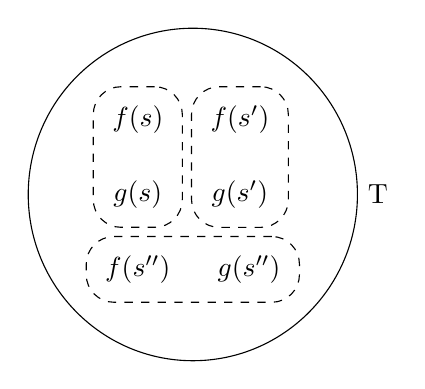
\begin{tikzpicture}
    [
        group/.style={ellipse, draw, minimum height=20pt,
                      minimum width=50pt, label=right:#1},
        subgroup/.style={rounded corners=10, draw, dashed},
        dot/.style={circle, fill, minimum width=2.5pt, inner sep=0pt}
    ]
    \node (fs) {$f(s)$};
    \node (gs) [below=10pt of fs] {$g(s)$};
    \node (fsp) [right=10pt of fs] {$f(s')$};
    \node (gsp) [below=10pt of fsp] {$g(s')$};
    \node (fspp) [below=10pt of gs] {$f(s'')$};
    \node (gspp) [right=10pt of fspp] {$g(s'')$};
    \node (s) [fit=(fs) (gs), subgroup] {};
    \node (sp) [fit=(fsp) (gsp), subgroup] {};
    \node (spp) [fit=(fspp) (gspp), subgroup] {};
    \node [fit=(s) (sp) (spp), group=T] {};
\end{tikzpicture}
\end{center}

Moreover, if, for example, $f(s)$ was equal to $g(s')$, we would like all of
$f(s)$, $g(s)$, $f(s')$ and $g(s')$ to be equal -- or, at least, equivalent.
This suggests defining an equivalence relation ensuring that the above elements
all reside in the same equivalence class. The function $\kappa$ would then map
every element $t \in T$ to its corresponding equivalence class in $K$, and
therefore $K$ would be the \emph{quotient set} of $T$ by the equivalence
relation.

Concretely, define the relation $ {}_{f}\hspace{-3px}\sim_{g}\ \subseteq T
\times T$ as:

\begin{equation*}
    {}_{f}\hspace{-3px}\sim_{g}\ 
    \eqdef\ 
    \bigsetof{\,\big(f(s), g(s)\big) \suchthat s \in S\,}
\end{equation*}
and let ${}_{f}\hspace{-3px}\approx_{g}$ be the least equivalence relation
that contains ${}_{f}\hspace{-3px}\sim_{g}$. That is, 
$x\: {}_f\hspace*{-3px}\approx_g y$ iff there is a finite sequence of elements
$z_0, z_1, \ldots, z_n$~$(n\in\nats)$ such that 
\[
 x = z_0\ 
 {}_f\hspace*{-3px}\sim_g 
 z_1 \
 {}_f\hspace*{-3px}\sim_g 
 \ \cdots \
 {}_f\hspace*{-3px}\sim_g 
 z_{n-1}\
 {}_f\hspace*{-3px}\sim_g 
 z_n = y
 \enspace.  
\]
Now, we define the coequaliser $\kappa$ of $f$ and $g$ as a function from $T$
to the quotient set $T_{\mbox{/${}_f\hspace*{-3px}\approx_g$}}$, the set of
equivalence classes of $T$ under ${}_f\hspace*{-3px}\approx_g$:

\begin{center}
\begin{tikzcd}[row sep=0.2em]
      S \arrow[r, shift left=5pt, "f"]
        \arrow[r, shift right=5pt, swap, "g"]
    & T \arrow[r, "\kappa"]
    & T_{\mbox{/${}_f\hspace*{-3px}\approx_g$}}
    \\
    {}
    & t \arrow[r, mapsto]
    & \left[ t \right]_{ {}_f\hspace*{-0px}\approx_g }
\end{tikzcd}
\end{center}

\begin{exercise}
    Show that this definition has the universal property of coequalisers.
\end{exercise}

\section{Pushouts}

Consider the following diagram, called a \emph{span}:

\begin{center}
\begin{tikzcd}
    C \arrow[r, "g"] \arrow[d, "f", swap]
    & B
    \\
    A
\end{tikzcd}
\end{center}

To define its colimit, called a \emph{pushout}, we again consider the required
commuting cocones:

\begin{center}
\begin{tikzcd}
    C \arrow[r, "g"] \arrow[d, "f", swap] \arrow[rd, "\gamma"]
    & B \arrow[d, "\beta"]
    \\
    A \arrow[r, "\alpha"]
    & K
\end{tikzcd}
\end{center}

We require this diagram to commute, 
\ie~$\alpha \comp f = \beta \comp g = \gamma$; again, $\gamma$ can be defined
from $\alpha$ or $\beta$ so it is usually omitted).  We also require the
pushout to be the universal initial solution: for all other cocones (also
called \emph{cospans}) $(u: A\to X\leftarrow B: v)$, there is a unique map
from $K$ to $X$ such that the following diagram commutes:
\begin{center}
\begin{tikzcd}
    C \rar{g} \dar[swap]{f}
    & B \arrow[d, "\beta"] \arrow[ddr, bend left=30, "\forall v"] &[-0.5em] {}
    \\
    A \arrow[r, "\alpha"] \arrow[rrd, bend right=30, "\forall u"]
    & K \arrow[rd, dashed, "\exists! w"] & {}
    \\[-0.5em]
    && \forall X
\end{tikzcd}
\end{center}

The following notation is used for pushouts:
\begin{center}
\begin{tikzcd}
    C \rar{g} \dar{f} \arrow[dr, phantom, "\ulcorner" font=\Large, very near end]
    & B \dar{\beta}
    \\
    A \rar[swap]{\alpha}
    & K
\end{tikzcd}
\end{center}

\paragraph{Pushouts from coproducts and coequalisers.}

The above looks similar to the coproduct diagram, so our initial guess to
construct a pushout could be to take $A + B$:

\begin{center}
\begin{tikzcd}
    C \rar{g} \dar[swap]{f}
    & B \arrow[d, "\iota_2", dotted]
    \\
    A \arrow[swap,r, "\iota_1", dotted]
    & A + B
\end{tikzcd}
\end{center}

However, this diagram does not necessarily commute: there is no reason for
which $\iota_1 \comp f = \iota_2 \comp g$ in general.  The trick is then to
universally force this commutativity by means of the coequaliser 
$c = \text{coeq} (\iota_1 \comp f,\ \iota_2 \comp g )$:

\begin{center}
\begin{tikzcd}
    C \rar{g} \dar[swap]{f}
    & B \arrow[d, "\iota_2", dotted] \arrow[ddr, bend left=30, "\beta"]
    &[-0.5em] {}
    \\
    A \arrow[r, "\iota_1", dotted] \arrow[drr, bend right=30, "\alpha"]
    & A + B \arrow[rd, "c"] & {}
    \\[-0.5em]
    && K
\end{tikzcd}
\end{center}

\exercise{ 
  Show that the above construction yields a pushout.
}

\begin{example}
In $\catset$, the pushout is then a quotient set (by the appropriate
equivalence relation) of the disjoint union of $A$ and $B$.
\begin{center}
\begin{tikzcd}
    C \rar \dar \arrow[dr, phantom, "\ulcorner" font=\Large, very near end]
    & B \dar
    \\
    A \rar
    & (A \uplus B)_{\mbox{\hspace*{-1mm}/$\approx$}}
\end{tikzcd}
\end{center}
\end{example}

\section{Finite colimits}

So far we looked at special cases of colimits for $\omega$-chains, countable
sums, coequalisers and pushouts. However, the construction we saw in the
previous section can be applied to any finite diagram to find its colimit.

\begin{proposition}
If a category has initial object, binary sums, and coequalisers, then all
finite diagrams have a colimit.
\end{proposition}

In fact, we can state a more general result:

\begin{proposition}
If a category has all small coproducts and coequalisers, all small diagrams
have a colimit.
\end{proposition}

To demonstrate this, consider an arbitrary diagram such as this one:

\begin{center}
\begin{tikzcd}
C \arrow[r,"g"] \arrow[d,"f",swap] & B \arrow[r,"j"] \arrow[d,"i"] & E \\
A & D &
\end{tikzcd}
\end{center}

The ``algorithm'' for finding its colimit is simply a repetition of the
construction we performed for pushouts.  First we consider the sum
$K=A+B+C+D+E$.  To make the family 
\begin{center}\begin{tikzcd}[column sep=3em, row sep=2.5em]
  A 
  \arrow[swap,drr,"\iota_A"] 
  & B 
  \arrow[dr,"\iota_B"] 
  & C 
  \arrow[d,"\iota_C"] 
  & 
  D 
  \arrow[dl,"\iota_D",swap] 
  & E 
  \arrow[dll,"\iota_E"] 
  \\
  && K &&&
\end{tikzcd}\end{center}
into a cocone for the diagram, we repeatedly enforce compatibility with each
of the arrows in the diagram by means of coequalisers.
\begin{itemize}
\item
  To enforce compatibility with $f: C\to A$, we take the coequaliser
  \begin{center}\begin{tikzcd}[row sep=0em]
    C 
    \arrow[rd,"f",swap]
    \arrow[rr,shift left=10pt,"\iota_C"]
    & 
    & K \arrow[r,two heads,"\kappa_f"] & K_f
    \\
    & A \arrow[ru,"\iota_A",swap] & 
  \end{tikzcd}\end{center}

\item
  To further enforce compatibility with $g:C\to B$, we take the coequaliser
  \begin{center}\begin{tikzcd}[row sep=0em]
    C 
    \arrow[rd,"g",swap]
    \arrow[rr,shift left=10pt,"\kappa_f\comp\iota_C"]
    & 
    & K_f \arrow[r,two heads,"\kappa_{g}"] & K_{f,g}
    \\
    & B \arrow[ru,"\kappa_f\comp\iota_B",swap] & 
  \end{tikzcd}\end{center}

\item
  To further enforce compatibility with $i:B\to D$, we take the coequaliser
  \begin{center}\begin{tikzcd}[row sep=0em,column sep=3em]
    B 
    \arrow[rd,"i",swap]
    \arrow[rr,shift left=10pt,"\kappa_g\comp\kappa_f\comp\iota_B"]
    & 
    & K_{f,g} \arrow[r,two heads,"\kappa_i"] & K_{f,g,i}
    \\
    & D \arrow[ru,swap,"\kappa_g\comp\kappa_f\comp\iota_D"] & 
  \end{tikzcd}\end{center}

\item
  Finally, to further enforce compatibility with $j:B\to E$, we take the
  coequaliser 
  \begin{center}\begin{tikzcd}[row sep=0em,column sep=3em]
    B 
    \arrow[rd,"j",swap]
    \arrow[rr,shift
    left=10pt,"\kappa_i\comp\kappa_g\comp\kappa_f\comp\iota_B"
    ]
    & 
    & K_{f,g,i} \arrow[r,two heads,"\kappa_j"] & K_{f,g,i,j}
    \\
    & E
    \arrow[ru,swap,"\kappa_i\comp\kappa_g\comp\kappa_f\comp\iota_E"] 
    & 
  \end{tikzcd}\end{center}
\end{itemize}
The family 
\[
  \bigsetof{\,
  \kappa_j\comp\kappa_i\comp\kappa_g\comp\kappa_f\comp\iota_X 
  : X\to K_{f,g,i,j}
  \,}_{X\in\setof{A,B,C,D,E}}
\]
is a colimiting cocone.

Alternatively, we could have done the above construction ``in parallel'' with
just one coequalizer:
\begin{center}\begin{tikzcd}
\dom(f)+\dom(g)+\dom(i)+\dom(j)
\arrow[rr,shift left=10pt,"{[\,\iota_A\comp f\,,\,\iota_B\comp
  g\,,\,\iota_D\comp i\,,\,\iota_E\comp j\,]}"]
\arrow[swap,rr,shift
right=10pt,"{[\,\iota_C\,,\,\iota_C\,,\,\iota_B\,,\,\iota_B\,]}"]
&& 
A+B+C+D+E
\arrow[r,two heads,"q"]
& 
Q
\end{tikzcd}\end{center}
obtaining the colimiting cocone
\[
  \bigsetof{\, q\comp\iota_X : X\to Q \,}_{X\in\setof{A,B,C,D,E}}
\]


\chapter{Limits}
\lecturedetails{14 November 2017}{M Fiore, N Licker, S Borgeaud}

\section{Products}

Recall that in a category with products, we have a $\prod_{i \in I} X_i$
together with 
\begin{center}
  \begin{tikzcd}
    \prod_{i \in I} X_i
      \arrow["\pi_k"]{d}
    \\
    X_k
  \end{tikzcd}
\end{center}
for all $k \in I$.

\section{Equalizers}

An \emph{equalizer} of a parallel pair $f,g: A\to B$ is an object $E$ and a
morphism $e: E \to A$ such that $fe=ge$ and for all objects $X$ and morphisms
$x: X \to A$ satisfying $fx=gx$, there is a unique $u: X \to E$ such that
$eu = x$.

\begin{center}
  \begin{tikzcd}
    E
      \arrow["e"]{r}
    &
    A
      \arrow["f"above, shift left=+1]{r}
      \arrow["g"below, shift left=-1]{r}
    &
    B
    \\
    &
    \stackrel{\mbox{$X$}}\forall 
      \arrow["\forall x",swap]{u}
      \arrow["\exists! u", dotted]{ul}
    &
  \end{tikzcd}
\end{center}

\begin{example}
In $\catset$, $E = \bigsetof{ a \in A \mid f(a) = g(a) }\hookrightarrow A$ is
an equalizer of $f,g:A\to B$. 
\end{example}

\section{Pullbacks}

Pullbacks are limits of diagrams of the form:
\begin{center}
  \begin{tikzcd}
    &
    B
      \arrow["g"]{d}
    \\
    A
      \arrow["f"]{r}
    &
    C
  \end{tikzcd}
\end{center}
A span $A\stackrel p\longleftarrow P\stackrel q\longrightarrow B$ is a
\emph{pullback} of the cospan $(f:A \to C\leftarrow B: g)$ if for all spans
$A\stackrel u\longleftarrow X\stackrel v\longrightarrow B$ such that $fu=gv$,
there is a unique $w:X \to P$ such that $pw=u$ and $qw=v$:
\begin{center}
  \begin{tikzcd}
    X
      \arrow["\exists!w", dotted]{dr}
      \arrow["v", bend left=20]{drr}
      \arrow["u", bend right=20]{ddr}
    &
    &
    \\
    &
    P
      \arrow["q"]{r}
      \arrow["p"]{d}
      \arrow[phantom, "\lrcorner", pos=0]{dr}
    &
    B
      \arrow["g"]{d}
    \\
    &
    A
      \arrow["f"]{r}
    &
    C
  \end{tikzcd}
\end{center}

\begin{example}
In $\catset$, $P = \bigsetof{(a, b) \in A \times B \mid f(a) = g(b) }$,
together with the projections to $A$ and $B$, is a pullback of
$(f:A \to C\leftarrow B: g)$.
\end{example}

\begin{lemma}[Pullback Lemma]
For a commutative diagram
\begin{center}
\begin{tikzcd}
  \bullet \arrow[d] \arrow[r] & \bullet 
  \arrow[phantom, "\lrcorner", pos=0]{dr} \arrow[r] \arrow[d] & \bullet 
  \arrow[d] 
  \\ 
  \bullet \arrow[r] & \bullet \arrow[r] & \bullet 
\end{tikzcd}
\end{center}
where the right square is a pullback, the left square is a pullback if and
only iff so is the outer rectangle.
\end{lemma}

\begin{exercise}
	Proof the Pullback Lemma.
\end{exercise}


\section{Limits of diagrams}

\begin{definition}
A \emph{diagram} of shape a small category $\mathbb{G}$ in a category
$\mathcal{C}$ is a functor $\mathbb{G} \xrightarrow{D} \mathcal{C}$.
\end{definition}

\begin{example}
Diagrams for a discrete shape $\mathbb{G}$ (\ie~categories with only identity
arrows) amount to families of objects $\setof{  D_n }_{n \in \mathbb{G}}$ and
provide diagrams for [co]products.
\end{example}

\begin{example}
Diagrams for equalisers are of shape
\begin{center}\begin{tabular}{|c|}\hline
  \begin{tikzcd}
  \bullet
    \arrow[shift left=+1.5]{r}
    \arrow[shift left=-1.5]{r}
  &
  \bullet
  \end{tikzcd}\\ \hline
  \end{tabular}\end{center}
\end{example}

\begin{example}
Diagrams for pullbacks are of shape
  \begin{center}\begin{tabular}{|c|}\hline
    \begin{tikzcd}
      &
      \bullet
        \arrow[]{d}
      \\
      \bullet
        \arrow[]{r}
      &
      \bullet
    \end{tikzcd}\\ \hline\end{tabular}
  \end{center}
\end{example}

\begin{definition}
A \emph{cone} for a diagram $D:\mathbb{G} \to \mathcal{C}$ consists of:
\begin{itemize}
\item an object $X \in \mathcal{C}$
\item together with a family 
$\chi = \setof{\chi_n: X \to Dn}_{n \in \mathbb{G}}$ such that for all 
$m \xrightarrow{e} n$ in $\mathbb{G}$ the diagram 
\begin{center}
  \begin{tikzcd}
    D m
      \arrow["D e"]{rr}
    &
    &
    D n
    \\&&\\
    &
    X
      \arrow["\chi_m"]{uul}
      \arrow["\chi_n",swap]{uur}
    &
  \end{tikzcd}
\end{center}
commutes
\end{itemize}

A \emph{limit} of $D: \mathbb{G} \to \mathcal{C}$ is a terminal cone; that is,
a cone 
\[
\big(L, \lambda = \big\{ \lambda_m: L \to D m \big\}_{m \in \mathbb{G}}\big)
\]
such that for all cones
$\big(X, \chi = \big\{ \chi_m: X \to D m \big\}_{m \in \mathbb{G}}\big)$,
there is a unique $u$ making the following diagram commute:
\begin{center}
  \begin{tikzcd}
    X
      \arrow["\exists!u"]{rr}
      \arrow["\chi_m"below]{rdd}
    &
    &
    L
      \arrow["\lambda_m"]{ldd}
    \\&&\\
    &
    D m
    &
  \end{tikzcd}
\end{center}
\end{definition}

\begin{proposition}
A category with small products and equalizers has all small limits.
\end{proposition}
\begin{proof}[Proof idea]
For a diagram $D$ of shape $\mathbb{G}$, consider the construction
\begin{center}
  \begin{tikzcd}
    L
      \arrow["\text{eq}"]{r}
    &
    \prod_{k\in\mathbb{G}}{D k}
      \arrow
        [
          "{\langle D(e) \comp \pi_m\rangle_{e:m\to n}}"above,
          shift left=+1
        ]
        {rrr}
      \arrow
        [
          "{\langle \pi_n \rangle_{e:m\to n}}"below,
          shift left=-1
        ]
        {rrr}
    &
    &
    &
    \prod_{(e:m\to n) \in \mathbb{G}}
    D n
  \end{tikzcd}
\end{center}

The limit is then given by the family
\begin{center}$ 
\lambda =
\big\{
  \begin{tikzcd}
    L
      \arrow["{\text{eq}}",swap]{r}
      \arrow["\lambda_i"above , bend left=20]{rr}
    &
    {\prod_{k\in\mathbb G} D k}
      \arrow["{\pi_i}",swap,r]
    &
    D i 
  \end{tikzcd}
\big\}_{i\in\mathbb{G}}
$\end{center}
which is a cone because the diagram 
\begin{center}
  \begin{tikzcd}[row sep=5em]
    L
      \arrow["\text{eq}"]{r}
      \arrow[shift left=-1,"D(e)\comp\lambda_m",bend right]{drrr}
      \arrow[shift left=+1,"{\lambda_n}",swap,bend right]{drrr}
    &
    \prod_{k\in\mathbb{G}}{D k}
      \arrow
        [
          "{\langle D(e) \comp \pi_m\rangle_{e:m\to n}}"above,
          shift left=+1
        ]
        {rrr}
      \arrow
        [
          "{\langle \pi_n \rangle_{e:m\to n}}"below,
          shift left=-1
        ]
        {rrr}
      \arrow[shift left=-1,"D(e)\comp\pi_m"]{drr}
      \arrow[shift left=+1,"{\pi_n}",swap]{drr}
    &
    &
    &
    \prod_{(e:m\to n) \in \mathbb{G}}
    D n
    \arrow["\pi_{(e:m\to n)}"]{dl}
    \\
    & & & 
    Dn
    & 
  \end{tikzcd}
\end{center}
commutes for all $e:m\to n$ in $\mathbb G$.

It remains to show the universal property, which is left as an
\textbf{exercise}.
\end{proof}

\begin{lemma}
If a category has pullbacks and terminal object, then it has finite products.
\end{lemma}
\begin{proof}[Proof idea]
For every pullback diagram
\begin{center}
  \begin{tikzcd}
    P
      \arrow[phantom, "\lrcorner", pos=0]{dr}
      \arrow[]{r}
      \arrow[]{d}
    &
    B
      \arrow[]{d}
    \\
    A
      \arrow[]{r}
    &
    1
  \end{tikzcd}
\end{center}
the span
\begin{center}
  \begin{tikzcd}
    &
    P
      \arrow[""]{dl}\arrow[""]{dr}
    &
    \\
    A
    &
    &
    B
  \end{tikzcd}
\end{center}
is a product.
\end{proof}

\begin{lemma}
If a category has pullbacks and terminal object, then it has equalizers.
\end{lemma}
\begin{proof}[Proof idea]
Every pullback 
\begin{center}
  \begin{tikzcd}
    E
      \arrow[phantom, "\lrcorner", pos=0]{dr}
      \arrow["e"]{r}
      \arrow["e"left]{d}
    &
    A
      \arrow["{\langle id_A, g \rangle}"]{d}
    \\
    A
      \arrow["{\langle id_A, f \rangle}"below]{r}
    &
    A \times B
  \end{tikzcd}
\end{center}
gives the equalizer diagram 
\begin{center}
  \begin{tikzcd}
    E
      \arrow["e"above]{r}
    &
    A
      \arrow["f"above, shift left=+1]{r}
      \arrow["g"below, shift left=-1]{r}
    &
    B
  \end{tikzcd}
\end{center}
\end{proof}

\begin{remark}
In $\catset$, the above construction describes the equalizer
\[
  \bigsetof{\,a\in A\ \mbox{\Large$\mid$}\ f(a) = g(a)\,}
\]
by constructing the isomorphic set
\[
  \bigsetof{\, 
    (a, a')\in A\times A\ 
    \mbox{\Large$\mid$}\
    \big(a, f(a)\big) = \big(a', g(a')\big)
    \,}
  \enspace.
\]
\end{remark}

\section{Inverse images}

\begin{proposition}
In a pullback
\begin{center}
\begin{tikzcd}
P \arrow[r] \arrow[d, "p"'] \arrow[phantom, "\lrcorner", pos=0]{dr}  & 
S \arrow[d, "m",tail] 
\\ A \arrow[r] & B
\end{tikzcd}
\end{center}
where $m: S \to B$ is a monomorphism, necessarily so is $p: P \to A$.
\end{proposition}

\begin{remark}
Intuitively, monomorphisms are injective maps and therefore they are like
predicates: they select a subset of the elements in the range. 

In $\catset$, we have the pullback 
\begin{center}
\begin{tikzcd}
\bigsetof{\, (a,s)\in A\times S \suchthat f(a) = m(s) \,}  
\arrow[r] \arrow[d,tail] \arrow[phantom, "\lrcorner", pos=0]{dr}  & 
S \arrow[d, "m", tail] \\
A \arrow[r, "f"'] & B
\end{tikzcd}
\end{center}
and since 
\[ 
  \bigsetof{\, (a,s)\in A\times S \suchthat f(a) = m(s) \,} 
  \ \iso \
  \bigsetof{\, a\in A \suchthat f(a) \in m[S] \,} 
  \ = \
  f^{-1}\big(m[S]\big)
  \enspace,
\]
where $m[S]\eqdef\bigsetof{m(s)\in B\suchthat s\in S}\subseteq B$ is the image
of $S$ under $m$, we also have the pullbacks 
\begin{center}
\begin{tikzcd}
f^{-1}\big(m[S]\big) 
\arrow[r] \arrow[d, hook] \arrow[phantom, "\lrcorner", pos=0]{dr}  
& S \arrow[d,"m",tail] 
\\
A \arrow[r, "f"'] & B
\end{tikzcd}
\qquad and \qquad
\begin{tikzcd}
f^{-1}\big(m[S]\big) 
\arrow[r] \arrow[d, hook] \arrow[phantom, "\lrcorner", pos=0]{dr}  
& m[S] \arrow[d,hook] 
\\
A \arrow[r, "f"'] & B
\end{tikzcd}
\end{center}

Hence, again intuitively, pullbacks of monomorphisms along a map are like
inverse images.

For instance, note that for a morphism $f: A \to B$ we have the pullback
\begin{center}
\begin{tikzcd}
A \arrow[r, "f"] \arrow[d, "id_A",swap,tail]  
\arrow[phantom, "\lrcorner", pos=0]{dr} 
& B \arrow[d, "id_B",tail] \\
A \arrow[r, "f"'] & B
\end{tikzcd}
\end{center}
which abstractly captures the set-theoretic fact that $f^{-1}(B) = A$ for all
functions $f$.

We also have the set-theoretic fact that, for all functions $f:A\to B$ and
$g:B\to C$, 
\[
  (g \circ f)^{-1}(S) 
  \,=\,
  f^{-1}\big(g^{-1}(S)\big) 
  \enspace\text{for all $S\subseteq C$}
\]
that abstractly corresponds to the half of the Pullback Lemma that asserts
that, if 
\begin{center}
\begin{tikzcd}
f^{*}\big(g^{*}(S)\big) 
\arrow[phantom, "\lrcorner", pos=0]{dr} 
\arrow[r] 
\arrow[d,tail] & 
g^{*}(S) \arrow[d,tail] 
\\
A \arrow[r, "f"'] & B 
\end{tikzcd}
\qquad and \qquad
\begin{tikzcd}
g^{*}(S) \arrow[r] \arrow[d,tail]
\arrow[phantom, "\lrcorner", pos=0]{dr} 
& 
S \arrow[d, tail] 
\\
B \arrow[r,"g"'] & C	
\end{tikzcd}
\end{center}
are pullbacks, then so is
\begin{center}
\begin{tikzcd}
f^{*}\big(g^{*}(S)\big) 
\arrow[phantom, "\lrcorner", pos=0]{dr} 
\arrow[r] 
\arrow[d,tail] & g^{*}(S) \arrow[r] & 
S \arrow[d, tail] 
\\
A \arrow[r, "f"'] & B \arrow[r,"g"'] & C	
\end{tikzcd}
\end{center}
\end{remark}

\section{Subobjects}

\begin{proposition}
A morphism $m: A \to B$ is a monomorphism iff 
\begin{center}
\begin{tikzcd}
A \arrow[r, "id_A"] \arrow[d, "id_A"'] \arrow[phantom, "\lrcorner", pos=0]{dr}
& A \arrow[d,"m"] \\ A \arrow[r, "m",swap] & B
\end{tikzcd}	
\end{center}
is a pullback
\end{proposition}

\begin{exercise}
	Prove the proposition.
\end{exercise}

\begin{definition}[Monomorphism equivalence]
Given two monomorphisms $m_1: S_1 \to A$ and $m_2: S_2 \to A$; that is,
	\begin{center}
		\begin{tikzcd}
S_1 \arrow[rd, "m_1"', tail] &  & S_2 \arrow[ld, "m_2", tail] \\
 & A & 
\end{tikzcd}
	\end{center}
\end{definition}
we say $m_1 \approx m_2$ holds iff there exists a (necessarily unique)
isomorphism $S_1 \stackrel\iso\longrightarrow S_2$ such that the diagram
\begin{center}
\begin{tikzcd}
S_1 \arrow[rd, "m_1"', tail] \arrow[rr, "\cong"] &  & S_2 \arrow[ld, "m_2", tail] \\
 & A & 
\end{tikzcd}
\end{center}
commutes.

\begin{definition}[Suboject]
A \emph{suboject} of an object $A$ is an equivalence class $[m]_{\approx}$ for
$m$ a monomorphism into $A$.  
\end{definition}

\begin{definition}[Subobject functor]
For a category $\mathcal{C}$ with pullbacks we have a 
\emph{subobject functor}
\[
\mathrm{Sub}: \mathcal{C}^\op \to  \catset 
\]
mapping objects
\begin{center}
\begin{tikzcd}[column sep=small]
X \arrow[rr, maps to] &  & 
\mathrm{Sub}(X) 
\eqdef \bigsetof{\, [m]_{\approx} \mid m \text{ is a monomorphism into } X \,}  
\end{tikzcd}
\end{center}
and mapping a morphism $f: Y \to X$ in $\mathcal C$ to the function
$\mathrm{Sub}(f): \mathrm{Sub}(X) \to \mathrm{Sub}(Y)$ given by
\begin{center}
\begin{tikzcd}
\lbrack m \rbrack_{\approx} \arrow[r, maps to] & \lbrack f^*(m)\rbrack_{\approx}
\end{tikzcd}
\end{center}
for a pullback square
\begin{center}
\begin{tikzcd}
f^*(S) \arrow[r] \arrow[d, "f^*(m)"', tail] 
\arrow[phantom, "\lrcorner", pos=0]{dr} & S \arrow[d, "m", tail] \\
Y \arrow[r, "f"'] & X
\end{tikzcd}
\end{center}
\end{definition}
\begin{remark}
Functoriality follows from the pullback lemma.	
\end{remark}

\begin{example}
In $\catset$, two injections into the same set are equivalent iff they have
the same image, and $\mathrm{Sub}$ is naturally isomorphic to the
contravariant powerset functor (with action given by inverse image).
\end{example}

\begin{exercise}
What is a representation 
\begin{center}
\begin{tikzcd}
\mathcal{C}(\phold,\Omega) \arrow[r, "\iso", Rightarrow] &
\mathrm{Sub}(\phold)
\end{tikzcd}
\end{center}	
for $\mathrm{Sub}$?
\end{exercise}
 

\chapter{Adjoint Functors}
\lecturedetails{16 November 2017}{M Fiore, R Kusztos}

\section{More about subobjects classifiers}

Recall the definition of the \underline{Sub} functor: 

\begin{align*}
  \underline{Sub}: \lscat{C}^{op} &\longrightarrow \textbf{Set} \\
  X &\longmapsto \underline{Sub}(X) = \bigl\{ [m]_{\approx} | 
    \textrm{m is mono into X} \bigl\} \\ 
\end{align*}

\begin{center}
  \begin{tikzcd}
    f^{*}(P)
      \arrow[phantom, "\lrcorner", pos=0]{dr} 
      \arrow[r] 
      \arrow[d] & 
    X 
      \arrow[d] \\
    P
      \arrow[r] & 
    Y
  \end{tikzcd}
\end{center}

What is a representation for this?
\begin{definition}[Subobject classifiers]
  To give a natural isomorphism, 
  $\lscat{C}(\_,\Omega) \overset{\iso}{\Longrightarrow} \underline{Sub}(\_) $ 
  is equivalent to giving an 
  $\Omega \in \lscat{C}$ 
  and a 
  $ \Bigl[t \underset{\Omega}{\overset{T}{\downarrow}} \Bigl] 
    \in \underline{Sub}(\Omega)$
  such that for all 
  $X \in \lscat{C}^{\Omega}$
  there exists a bijective correspondence: 

  \begin{align*}
    \forall 
    \Bigl[m \underset{X}{\overset{P}{\downarrow}} \Bigl] 
    \in \underline{Sub}(X) \quad
    \exists! 
    X \overset{\chi_{[m]}}{\longrightarrow} \Omega \quad 
    \textrm{such that} \quad
    \chi_{[m]}^{*}[t] = [m]
  \end{align*}
\end{definition}

\begin{definition}[Subobject classifiers]
  \label{subobject_classifier_def}
  The previous definition is equivalent to simply giving 
  $\Omega \in \lscat{C}$
  and 
  $t \underset{\Omega}{\overset{T}{\downarrow}} \in \lscat{C}$
  such that 
  \begin{align*}
    \forall 
    m \underset{X}{\overset{P}{\downarrow}}
    \in \underline{Sub}(X) \quad
    \exists! 
    X \overset{\chi_{m}}{\longrightarrow} \Omega
  \end{align*}  
  \begin{center}
    \begin{tikzcd}
    P 
      \arrow[phantom, "\lrcorner", pos=0]{dr} 
      \arrow[r, "u"] 
      \arrow[d, "m"] & 
    T 
      \arrow[d, "t"] \\
    X
      \arrow[r, "\chi_m"] & 
    \Omega
    \end{tikzcd}
    \end{center}
  for some $u$
\end{definition}

\begin{example}[in $\textbf{Set}$]
\begin{align*}
  1 \overset{t}{\longrightarrow} \{t, f\} = \Omega
\end{align*}
\begin{align*}
  Sub(X) = \mathcal{P}(X)
\end{align*}

\begin{center}
  \begin{tikzcd}
    P 
      \arrow[phantom, "\lrcorner", pos=0]{dr} 
      \arrow[r, "u"] 
      \arrow[d, "m"] & 
    1
      \arrow[d, "t"] \\
    X
      \arrow[r, "\exists!\varphi"] & 
    \{t, f\}
    \end{tikzcd}
  \end{center}

Where $\varphi$ is such that $\varphi^{-1}\{t\} = P$ \\
Since we are in set, $\varphi$ is the characteristic function of X

\begin{equation*}
 \varphi = \chi_m(x) = 
  \begin{cases}
    t & x \in P \\
    f & x \notin P 
  \end{cases}
\end{equation*}

\end{example}

\begin{exercise}
  In the subobject classifier definition 
  (Definition \ref{subobject_classifier_def}), $T$ is necessarily a
terminal object
\end{exercise}

\begin{definition}[Toposes]
  A topos is a category with: 
  \begin{itemize}
    \item all finite limits 
    \item exponentials
    \item subobject classifier $\Omega$
  \end{itemize}

Examples of toposes are: 
  \textbf{Set}, 
  $\textbf{Set}^{\mathbb{C}^{op}}$, 
  \textbf{DirGraph}

\end{definition}

\begin{remark}
  Toposes are models of Higher Intuitionistic Logic.
\end{remark}

\begin{exercise}
  What is $\Omega$ in \textbf{DirGraph}?

  For some graph 
  $G = (N, E)$, 
  Sub(G) = the set of all its subgraphs, each given by a subset of nodes,
  $S_n \subseteq N$
  and a subset of edges 
  $E_n \subseteq E$ 
  between nodes in $S_n$.

  \begin{center}
    \begin{tikzcd}
      \bullet 
        \arrow[rr, bend left] & {} \arrow[dd, hook'] & 
        \bullet \arrow[loop, looseness=4] &  &  &  & 
        \bullet \arrow[dd, hook'] \arrow[loop, looseness=4] \\
       &  &  &  &  &  &  \\
       & {} &  &  &  &  & {} \\
      \bullet \arrow[rr, bend left] 
      \arrow[rd, bend right] &  & 
      \bullet
        & {} 
      \arrow[rr] &  & {} & 
      \textcolor{green}{\bullet} 
      \arrow[loop left, green]
      \arrow[loop right, red]
      \arrow[bend left=20, blue]{d} \\
       & \bullet \arrow[ru, bend right] \arrow[lu, bend right] &  &  &  &  & 
       \textcolor{red}{\bullet} 
       \arrow[loop right, red]
       \arrow[bend left=20, blue]{u}
    \end{tikzcd}
  \end{center}
\end{exercise}

\begin{exercise}
  What is $\Omega$ in $\textbf{Set}^{(0 \to 1)}$, also known as the 
Sierpinski topos.
\end{exercise}

\section{Adjoint Functors}

\begin{example}
  In the first lecture we introduced the free functor which maps a set to 
the free monoid:

  \begin{align*}
    \textbf{Set} &\overset{F}{\longrightarrow} \textbf{Mon} \\
    S &\longmapsto (S^*, t, \circ)
  \end{align*}
  Similarly, we can introduce the forgetful functor U, which gives the set 
underlying a monoid.

\begin{center}
  \begin{tikzcd}[sep=3em]
    \textbf{Mon}
      \ar["U"{right}]{d} 
    \\
    \textbf{Set}
      \ar[bend left=40, "F"{left}]{u}
  \end{tikzcd}\\[1mm]
\end{center}

Here, we observe that:

\begin{align*}
  \textbf{Mon}(F(S), \underline{M}) &\cong_{nat} 
    \textbf{Set}(S, U(\underline(M))) \\
    \shortintertext{We write that:} \\
    F &\dashv U \\
    \intertext{To say that F and U are adjoints; F is called the left adjoint
    whereas U is called the right adjoint}
  \end{align*}
\end{example}

\begin{example}[Colimits]
  \begin{align*}
    \lscat{C} &\underset{\Delta}{\longrightarrow} \lscat{C}^\mathbb{G} \\ 
    X &\longmapsto \Delta(X): \mathbb{C} \to \lscat{G} \quad 
    \textrm{which maps} \quad
    e \overset{m}{\underset{n}{\downarrow}} \longmapsto
    \overset{x}{\underset{x}{\downarrow}}id
  \end{align*} 
That is, 
  \begin{align*}
    \textrm{For} \quad D \in \lscat{C}^\mathbb{G},  \quad
    &\varphi: D \Rightarrow \Delta(X) \\
    &\equiv \textrm{cocone with vertex x for diagram D} \\
    \lscat{C}(\underline{colim}D, X) &\cong 
      \lscat{C}^{\mathbb{G}}(D, \Delta(X)) \\ 
    \underline{colim} &\dashv \Delta \\ 
    \shortintertext{Dually,} \\ 
    \lscat{C}(X, \underline{lim}D) &\cong
      \lscat{C}^{\mathbb{G}}(\Delta(X), D) \\
    \Delta &\dashv \underline{lim}  
  \end{align*}

\end{example}

\begin{definition}[Adjoint Pair]
An adojoint pair of functors, $F \dashv G: \lscat{D} \to \lscat{C}$ consists
of: 
 \begin{center}
  \begin{tikzcd}
    \lscat{D} 
    \ar[bend left=20, "G"]{r} &
   \lscat{C} 
    \ar[bend left=20, "F"]{l}
  \end{tikzcd}
\end{center}
together with a natural isomorphism:
\begin{align*}
\lscat{D}(F C, D) &\cong 
  \lscat{C}(C, G D) \\ 
\end{align*}

Equivalently, to give a left adjoint $F$ to a functor 
$G: \lscat{D} \to \lscat{G}$
is to give for all $X \in \lscat{C}$
and object $F(x) \in \lscat{D}$
together with a map $X \underset{\eta_X}{\rightarrow} G(F(X)$
in $\lscat{C} $
such that: 
\begin{center}
    \begin{tikzcd}[ampersand replacement=\&]
    X \arrow[r, "\eta_X"]
    \arrow[dr, "\forall f"{left}] \&
    G(F(X)) \arrow[d, "G(f^\#)"] \& 
    F(X) \arrow[d, mapsto, "\exists! f^\#"] \\
    {} \& G(Y) \& Y
  \end{tikzcd} 
\end{center}
\end{definition}
\begin{proposition}
  Left adjoints preserve colimits and dually, right adjoints preserve limits.
\end{proposition}

\begin{example}
A functor $F: \lscat{C} \to \lscat{D}$ preserves sums if:

  \begin{center}
    \begin{tabular}[t]{lc}
    $\forall$ sums in $\lscat{C}$
    \begin{tikzcd}
      {} & A + B & {} \\
      A \ar["\iota_1"]{ru} & & B \ar["\iota_2"above]{lu} \\
    \end{tikzcd}
    ,
    \begin{tikzcd}
      {} & F(A + B) & {} \\
      F(A) \ar["F(\iota_1)"]{ru} & & F(B) \ar["F(\iota_2)"above]{lu} \\
    \end{tikzcd}
    is a sum in $\lscat{D}$.
    \end{tabular}
  \end{center}

If $\lscat{D}$ has sums, 

\begin{center}
  \begin{tikzcd}
    & F(A) + F(B) \ar["\cong", dotted]{d} & \\ 
    & F(A + B) & \\
    F(A) \ar["F(\iota_1)"]{ru} 
         \ar["\iota^{F(A), F(B)}_1", bend left=40]{ruu} & & 
    F(B) \ar["F(\iota_2)"]{lu}
         \ar["\iota^{F(A), F(B)}_2", bend right=40]{luu} \\
    

  \end{tikzcd}
\end{center} 

We need to show that $F(A) + F(B) \cong F(A + B)$. We have previously shown
that this is equivalent to showing that: 

\[ 
  \Efrac
    {F(A) + F(B) \to z}
    {F(A + B) \to z}
\]

Intuitively,

\LARGE\[
  \Efrac
  {
  \Efrac
    {F(A) + F(B) \to z} 
    { \Efrac 
      {F(A) \to z}  
      {A \to G z}
      \quad 
      \Efrac 
      {F(B) \to z}
      {B \to G z}
    }
  }
  {
    \Efrac 
    {A + B \to G z}
    {F(A + B) \to z}
  }
\]

\end{example}

\begin{example}
  Exponentials are adjoints.
  \begin{align*}
    \_ \times A &\dashv A \Rightarrow (\_) \\
    \lscat{C}(X (\times A), B) &\cong \lscat{C}(X, (A \Rightarrow) B)
  \end{align*}
\end{example} 

\chapter{Adjoint Functors in Logic}
\lecturedetails{21 November 2017}{M Fiore, B Hardy, O Richardson}

The agenda for the next couple of lectures is (1) to focus on the links to logic (which will be presented in an informal manner, and not in full generality), and (2) some examples and techniques for how to prove things with adjoint functors.

\section{Different Definitions of Adjunctions}
We will explore four equivalent definitions of adjoint functors; the first three will be given in this lecture, and the last one will be described later on, once we have more intuition and context.

\subsection{Definition By Isomorphism}
The first definition is the original one given in in the last lecture. Given two functors $F: \lscat{C} \to \lscat{D}$ and $U: \lscat{D} \to \lscat{C}$ (think of $F$ as the free functor, which creates the most general possible structure, and $U$ as forgetful) 
 \begin{center}
  \begin{tikzcd}
    \lscat{D} 
    \ar[bend left=20, "G"]{r} &
   \lscat{C} 
    \ar[bend left=20, "F"]{l}
  \end{tikzcd}
\end{center}
Recall that $U \vdash F$ if there is an isomorphism:
\begin{equation*}
\lscat{D}(F C, D) \cong 
  \lscat{C}(C, G D) \;.
\end{equation*}
which is natural in $C$ and $D$. In the isomorphism above, let's name the maps $\varphi$ and $\phi$, as in the diagram below.
\begin{center}
  \begin{tikzcd}
    \lscat{D}(FC, D)
    \ar[bend left=20, "\varphi"]{r} &
    \lscat{C}(C, UD)
    \ar[bend left=20,  "\phi"]{l}
  \end{tikzcd}
\end{center}
We can also view these equivalences as two bijective correspondances between morphisms:
\begin{align*}
\Efrac{ F C \overset{f}\longrightarrow D}
{C \underset{\varphi(f)}\longrightarrow UD}
&\hspace{2in}
\Efrac{F C \overset{f}\longrightarrow D \overset{h}\longrightarrow D'}
{C \underset{\varphi(f)}\longrightarrow UD \underset{\varphi(U h)}\longrightarrow UD'}
\end{align*}
The question now becomes: what does naturality in $C$ look like? For any morphism $h : C' \to C$ in $\lscat{C}$, naturality in $C$ amounts to a structure preserving commutativity condition on $\varphi$, as below
\begin{align*}
  \Efrac{F C' \overset{Fh}\longrightarrow F C \overset{f}\longrightarrow D}
  {C' \underset{h}\longrightarrow C \underset{\varphi(f)}\longrightarrow UD}
  &\hspace{2in}
  \Efrac{F C \overset{f}\longrightarrow D \overset{h}\longrightarrow D'}
    {C \underset{\varphi(f)}\longrightarrow UD \underset{\varphi(U h)}\longrightarrow UD'}
  \\[1em]
  \text{Naturality in $C$:}~~&\hspace{2in}~~\text{Naturality in $D$:} \\
  \varphi(f \comp F h) = \varphi(f) \comp h
  &\hspace{2in}
    \varphi(h \comp f) = Uh \comp \varphi(f)
\end{align*}

\begin{remark}
	To ``transpose'' an arrow is to move it from the top to the bottom of the equivalence (or vice versa). On the left, this amounts to applying $F$, and on the right it ammounts to applying $U$.
\end{remark}

\subsection{Definition by Units}

In particular, we can transpose identities, and so we have $\varphi(\id{FC}) = \eta_C$ satisfying, for any $f$,
\begin{equation*}
  \Efrac{FC' \overset{F f}\longrightarrow FC \overset{\id{}}\longrightarrow FC}
  {C' \underset{f}\longrightarrow C \underset{\eta_C}\longrightarrow UFC}\;.
\end{equation*} 



\begin{definition}[Adjunctions, version 2]
Putting that last fact differently, we have an equivalent definition of an
adjunction: to have an adunction $F \dashv U$ is to have for each $C$, $\eta_C$ such that
\begin{equation*}
  \Efrac{FC \overset{\id{}}\longrightarrow FC}
  {C \underset{\eta_C}\longrightarrow UFC}
\end{equation*} 
and
\begin{center}
\begin{tikzcd}
C \arrow[rdd, "\forall f"'] \arrow[rr, "\eta_C"] &  & UFC \arrow[ldd, "Uf^\#"] & UC \arrow[dd, "\exists!f^\#"] \\
 &  &  &  \\
 & UD &  & D
\end{tikzcd}
\end{center}
\end{definition}

Thus, an an adjunction can be specified by a family of identity transpose maps $\eta_C$.

\subsection{Definition by Counits}
\begin{definition}[Adjunctions, version 3]
Similarly, we can play the dual game to arrive at another equivalent defintion:
to have an adunction $F \dashv U$ is to have for each $D$, $\epsilon_D$ such that
\begin{equation*}
  \Efrac{FUD \overset{\epsilon_D}\longrightarrow D}
  {UD \underset{\id{}}\longrightarrow UD}
\end{equation*} 
and
\begin{center}
\begin{tikzcd}
UD & FUD \arrow[rr, "\varepsilon_D"] &  & D \\
 &  &  &  \\
C \arrow[uu, "\exists! \hat f"] &  & FC \arrow[luu, "F \hat f"] \arrow[ruu, "\forall f"'] & 
\end{tikzcd}
\end{center}
\end{definition}

\section{Adjoints Between Posets}
\begin{remark}
	Sometimes if struggling with understanding a category in full generality, one can take away structure, and think of it as an order or a monoid. 
\end{remark}
If we regard posets as categories, we can talk about adjunctions between them. note that adjuncts between posets are also called ``Galois connections'', and have applications in abstract interpretations.


Suppose we have
\begin{center}
\begin{tikzcd}
P \arrow[rr, "f", bend left] & \adjointDown & Q \arrow[ll, "g", bend left]
\end{tikzcd}
\end{center}
(recalling that functors $f,g$ between poset categories are monotone functions
between the posets).

Then to have the adjunction is to have
\begin{itemize}
\item From the bijection condition (definition 1)
\[\forall p \in P, q \in Q.\; f(p) \le_Q q \iff p \le_p g(q)\;;\]
\item by naturality in $p$, (or more clearly, units from definition 2)
\[\forall p \in P.\; p \le_P (f \comp g)(p)\;;\]
\item by naturality in $q$, (or more clearly, counits from definition 3)
\[\forall q \in Q.\; (f \comp g)(q) \le_Q q\;.\]
\end{itemize}

Now, suppose $P$ and $Q$ are complete (\ie they have all joins and meets).
Notice that $f$ preserves joins and $g$ preserves meets. Conversely (this only
works in $\catposet$), if $f : P \longrightarrow Q$ preserves joins then it has
a right adjoint, and if $g : Q \longrightarrow P$ preserves meets then it has a
left adjoint.

\emph{Proof}. Given $g : Q \longrightarrow P$, we need to define $f : P
\longrightarrow Q$ such that
\begin{center}
  \begin{tikzcd}
p \arrow[r, "f"] \arrow[d] & f(p) \arrow[d] \\
g(q) & q \arrow[l, "g"]
\end{tikzcd}
\end{center}
commutes.

\begin{exercise}
Check that the greatest lower bound $f$ and least upper bound $g$ 
\begin{align*}
	f &\eqdef \bigwedge \{q \in Q~|~ p \le g(q)\}\\
	g &\eqdef \bigvee \{p \in P~|~ f(p) \le q\}
\end{align*}
are adjoint.
\end{exercise}

\section{Adjoints as a basis for Existential/Universal Quantifies}
\begin{example}
  Let $X \overset{f}\longrightarrow Y$ be a function (in $\catset$). Because the
  inverse image $f^{-1}$ preserves both $\cup$ and $\cap$ (meets and joins), then by the above it must have both a right and a left adjoint functor. Hence we have arrows
  which we will call $\exists f$ and $\forall f$ satisfying
  \begin{center}
    \begin{tikzcd}
 &  & \adjointDown &  &  \\
\mathcal P(X) \arrow[rrrr, "\exists f", bend left=70] \arrow[rrrr, "\forall f"', bend right=70] &  &  &  & \mathcal P(Y) \arrow[llll, "f^{-1}"] \\
 &  & \adjointDown &  & 
\end{tikzcd}
  \end{center}

  \begin{exercise}
    Give explicit descriptions of $\exists f \dashv f^{-1} \dashv \forall f$.
  \end{exercise}

  \textbf{Example of the example.} Let's compute the adjoints in the special case of the above example, where $X = A \times B$, $Y = B$, and $f = \pi_2^{A,B}$.
  
  \begin{center}
    \begin{tikzcd}
 &  & \adjointDown &  &  \\
\mathcal P(A \times B) \arrow[rrrr, "\exists_A", bend left=70] \arrow[rrrr, "\forall_A"', bend right=70] &  &  &  & \mathcal P(B) \arrow[llll, "\pi_2^{-1}"] \\
 &  & \adjointDown &  & 
\end{tikzcd}
  \end{center}

\textbf{Idea.} Members of $\mathcal P(A \times B)$ can be seen as predicates/relations
over $A$ and $B$. Then, given some predicate $R(x^A, y^B)$ (read as $x$ fo type $A$, and $y$ of type $B$), $\exists_A$ and
$\forall_A$ give us predicates on just a variable in $B$:
\begin{align*}
  \exists_A(P)(y^B) & = \exists x \in A.~R(x, y) \\
  \forall_A(P)(y^B) & = \forall x \in A.~R(x, y).
\end{align*}

Notice that $\pi_2^{-1}(P) = \{(a, b) \in A \times B \;|\; b \in P\} \longrightarrow
P = A \times P$. Then to show that $\exists_A$ and $\forall_A$ are the required
adjoints is to show that

\[
  \Efrac{\exists_A(R) \subseteq P}{R \subseteq \pi_2^{-1}(P) = A \times P}
\]
and
\[
  \Efrac{A \times P = \pi_2^{-1}(P) \subseteq R}{P \subseteq \forall_A(R)}\;.
\]

Interestingly, this is a possible definition of quantifiers in terms of
adjoints [due to Lawvere].
\end{example}

\begin{remark}
 This works in every topos with \underline{Sub} (a subobject classifier), although the details are different.
\end{remark}

\section{Connectives and Slice Categories}

Observe the following two analogies

\begin{align*}
	\Efrac{C \to A \times B}{C \to A\quad C \to B} &\hspace{10em} \Efrac{\Gamma \vdash A \land B}{\Gamma \vdash A\quad \Gamma \vdash B} \\
	\Efrac{C \times A  \to B}{C \to A \Rightarrow B} &\hspace{10em} \Efrac{\Gamma, A \vdash B}{\Gamma \vdash A \Rightarrow B}
\end{align*}

\begin{remark}
	This generalizes in connection to type theory, with respect to slice categories (to be defined below), where $\exists_A$ becomes a $\Sigma$ type, and $\forall_A$ becomes a $\Pi$ type.
\end{remark}

\begin{definition}
	Given a category $\lscat{C}$ and an object $A \in \lscat C$, the \textit{slice of $\lscat C$ over $A$}, denoted $\sfrac{\lscat C}{ A}$, has
	\begin{align*}
		\textbf{objects:} \qquad & \left(X \in \lscat C, ~f\underset{A}{\overset{X}{\downarrow}} \right) \\
		\textbf{Morphisms:} \qquad & \left(X , ~f \underset{A}{\overset{X}{\downarrow}} \right) \overset{h}{\longrightarrow} \left(Y, ~g\underset{A}{\overset{Y}{\downarrow}} \right)\\
		& \text{ are maps $h: X \to Y$ such that } \\
		& \begin{tikzcd}[ampersand replacement=\&]
			 X \arrow[r, "h"] \arrow[dr, "f"'] \& Y \arrow[d, "g"] \\ \&A
		\end{tikzcd} \qquad\text{commutes}
	\end{align*}
\end{definition}

We also have a forgetful functor $\Sigma_A$, defined as follows
\begin{align*}
\sfrac{\lscat C }{A} &\overset{\Sigma_A}{\longrightarrow} \lscat C \\
\left(X , \underset{A}{\overset{X}{\downarrow}}f \right) &\longmapsto X
\end{align*}

\textbf{Proposition.} $\Sigma_A: \sfrac{\lscat C}{A} \to \lscat C$ has a right adjoint if and only if $\lscat C$ has products with A. \footnote{this condition was originally "$\lscat C$ has pullbacks along maps into $A$, but we didn't have time enough to do the more general result with this premise}

\begin{center}
	\begin{tikzcd}[column sep = huge, row sep=large]
		\sfrac{\lscat C}{A}
			\arrow[r, bend left= 50, "\Pi_A"{name=P, above}]
			\arrow[r, bend right=50, "\Sigma_A"{name=S, below}]
		 & \lscat C \arrow[l, "{(~)^*}"{name=M, description}]\\
		 \arrow[from={S}, to={M}, phantom, "\dashv" rotate=90 ]
		 \arrow[from={M}, to={P}, phantom, "\dashv" rotate=90 ]
		 
	\end{tikzcd}
\end{center}


In Type Theory, given a function $f: A \to B$ in $\lscat C$ that has pullbacks $f^*$ along $f$, then the sigma is left adjoint to $f^*$, and if we're lucky we will also have $\pi_f$, right adjoint $f^*$.
\begin{center}
	\begin{tikzcd}[column sep = huge, row sep=large]
		\sfrac{\lscat C}{A}
			\arrow[r, bend left= 50, "\Pi_f"{name=P, above}]
			\arrow[r, bend right=50, "\Sigma_f"{name=S, below}]
		& \sfrac{\lscat C}{B} \arrow[l, "{f^*}"{name=M, description}]\\
		\arrow[from={S}, to={M}, phantom, "\dashv" rotate=90 ]
		\arrow[from={M}, to={P}, phantom, "\dashv" rotate=90 ]
	\end{tikzcd}
\end{center}
The general idea is to replace the subobjects with slices and keep the pullbacks.
\begin{align*}
	\lscat C &\overset{(~)^*}{\longrightarrow} \sfrac{\lscat C }{A} \\
	X &\longmapsto \left(X \times A, \underset{A}{\overset{X \times A}{\downarrow}}\pi_2 \right)
\end{align*}


\end{document}
